\documentclass[a4paper, 11pt]{report}
\usepackage[utf8]{inputenc}
\usepackage[french]{babel}
\usepackage[T1]{fontenc}
\usepackage{amsmath}
\usepackage{amsfonts}
\usepackage{amssymb}
\usepackage{graphicx, float}
\usepackage{algorithm, algorithmic}
\usepackage{csquotes}
\usepackage{wasysym}
\usepackage{dsfont}
\usepackage{yhmath}
\usepackage{hyperref}
\usepackage{tabularx}
\usepackage{colortbl}
\usepackage{hhline}
\usepackage[left=2cm,right=2cm,top=2cm,bottom=2cm]{geometry}

\author{Guillaume Rochette}
\title{Stage de Fin d'Études
		\\
Création d'un Moteur de Recherche dans les Images Satellite}

\newcommand{\lexp}[1]{\phantom{}^{#1}}
\newcommand{\elem}[4]{\lexp{#2}#1^{#3}_{#4}}

\begin{document}
\maketitle
\tableofcontents
	
\chapter{Introduction}
\section{Présentation de l'Entreprise}
\subsection{Le Groupe Thales}
Le groupe Thales, historiquement fabricant d'électronique, est un acteur français majeur dans les secteurs de l'aéronautique, le spatial, la défense, la sécurité et le transport terrestre.
\begin{figure}[H]
	\begin{center}
		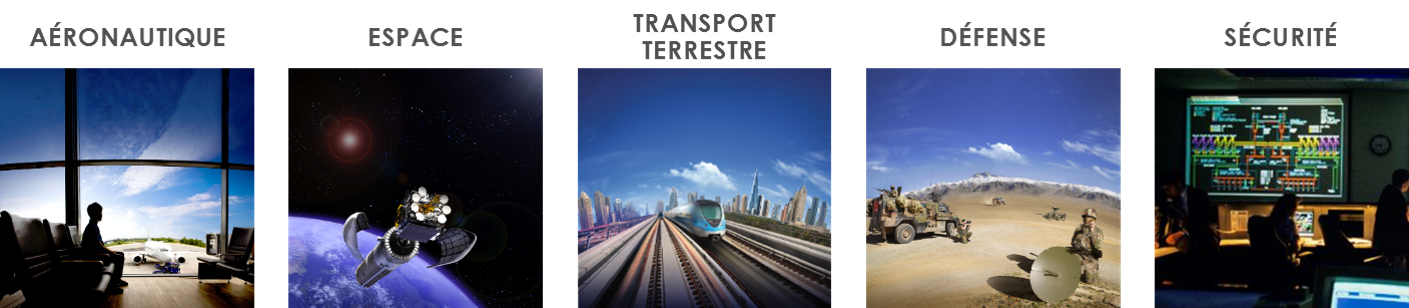
\includegraphics[scale=0.5]{Images/Secteurs_Activites.png}
		\caption{Secteurs d'activités de Thales}
	\end{center}
\end{figure}
Le groupe Thales est implanté dans $56$ pays et emploie $64000$ salariés, dont $34000$ collaborateurs répartis dans $70$ sites en France.
\begin{figure}[H]
	\begin{center}
		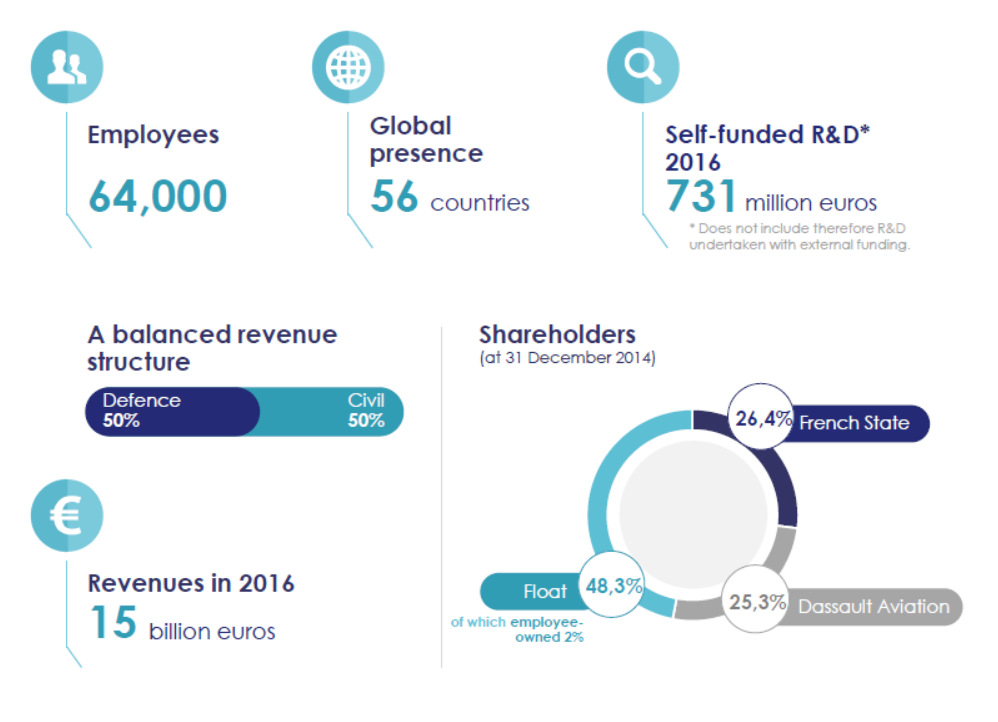
\includegraphics[scale=0.5]{Images/Chiffres_Cles.png}
		\caption{Chiffres Clés du Groupe Thales}
	\end{center}
\end{figure}
\subsection{Thales Services}
Thales Services est une entreprise spécialisée dans les activités de conception, développement et maintenance de systèmes informatiques sécurisés.

Elle est implantée sur tout le territoire français, chaque site ayant des spécialisations différentes.
\begin{figure}[H]
	\begin{center}
		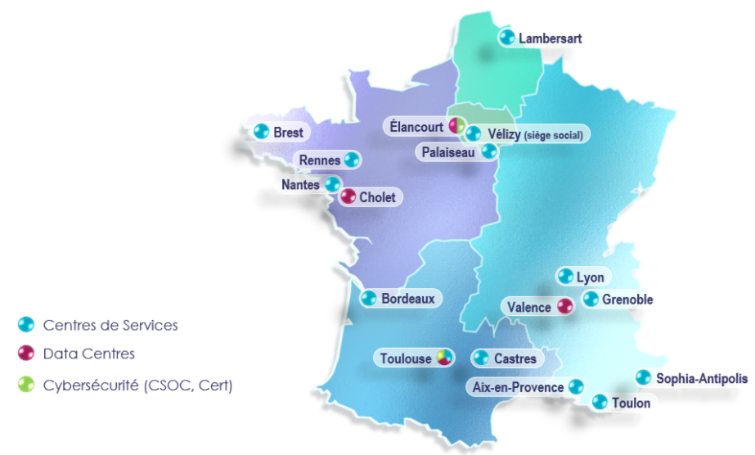
\includegraphics[scale=1.0]{Images/TS_France.png}
		\caption{Implantation de Thales Services en France}
	\end{center}
\end{figure}
Le groupe Thales, et par extension Thales Services, est organisé de façon \emph{matricielle}, c'est-à-dire par zones géographiques et par domaines d'activités.
\begin{figure}[H]
	\begin{center}
		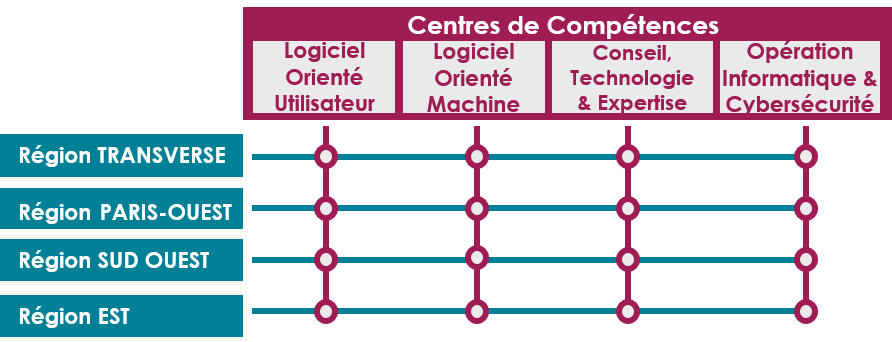
\includegraphics[scale=0.7]{Images/Matrice_Thales_Services.png}
		\caption{Organisation matricielle de Thales Services}
	\end{center}
\end{figure}
Ce stage s'effectue dans le \emph{Centre de Compétences} \textbf{Logiciel Orienté Machine} de la \emph{Région Sud-Ouest}.
\section{Objectifs du Stage}
La place de l'apprentissage profond grandit dans de nombreux domaines de l'industrie, et particulièrement dans les secteurs liés au traitement d'image.

Le potentiel de l'apprentissage profond à réaliser des tâches jugées trop complexes pour des algorithmes \emph{traditionnels} est immense.
Pour certaines applications de vision, les machines offrent aujourd'hui des performances supérieures à celles d'un humain.
Les avancées les plus spectaculaires à ce jour sont majoritairement réalisées sur des images provenant de la photographie grand-public, avec ses particularités et ses contraintes.

Thales Services, dont l'un des clients est le Centre National d'Études Spatiales (CNES), produit des suites de logiciels utilisés dans la chaîne de traitement d'images pour des satellites tels que Pléiades, SPOT ou encore Sentinel-2.

L'application de méthodes d'apprentissage profond à des images satellites est prometteuse mais encore peu utilisée, justifiant l'intérêt et la volonté de Thales Services de monter en compétence dans ce domaine.

Les objectifs de ce stage sont les suivants :
\begin{itemize}
	\item Apporter des connaissances relatives à l'apprentissage profond appliqué au traitement de l'image.
	\item Déterminer des opportunités d'application de vision par ordinateur pour des images satellite, telle que de la segmentation d'image ou de la recherche de similarités.
	\item Proposer et évaluer des modèles pour les applications proposées.
\end{itemize}

Dans le premier chapitre, nous aborderons l'imagerie spatiale, présentant ses enjeux, le fonctionnement général d'un satellite de télédétection, et enfin les caractéristiques et problématiques liées aux images satellite.

Dans le second chapitre, nous définirons l'apprentissage machine et ses concepts clés.

Dans le troisième chapitre, nous définirons précisément le domaine de l'apprentissage profond, nous expliquerons en détail le fonctionnement des réseaux de neurones, les motivations de cette discipline, ainsi qu'une explication détaillée des réseaux de neurones spécialisés dans le traitement des images

Dans le quatrième chapitre, nous ferons le lien entre apprentissage profond et imagerie spatiale, justifiant l'utilité d'appliquer le premier au second, ainsi que les applications réalisées au cours de ce stage permettant d'extraire des informations des images satellite. Les tâches que nous présenterons sont la segmentation d'images et la recherche de similarités.

\chapter{L'Imagerie Satellite}
De tout temps, l'humain a toujours souhaité pouvoir observer le monde, que ce soit à des fins militaires, scientifiques ou à simple but de contemplation.

Les besoins en matière de \emph{télédétection} sont plus anciens que les premiers satellites artificiels. Dès la fin du XIX ème siècle, lors du siège de Paris en $1870$, des ballons effectuaient des missions de reconnaissance en utilisant les progrès en matière de photographie.

Jusqu'aux années $1970$, la télédétection servait majoritairement à l'espionnage et la cartographie, principalement réalisée par le biais d'appareils photographiques emportés dans des avions.
Les premières images de la Terre depuis l'Espace ont été réalisées de cette même manière, des appareils photographiques à microfilm étaient embarqués dans des satellites artificiels. Il est à noter qu'un défi de taille était la réception de ces microfilms alors largués vers la Terre depuis l'Espace.

L'apparition de \emph{capteurs numériques} a révolutionné le domaine de la télédétection, car permettant de s'abstraire du support physique, problématique de par sa quantité limitée à bord, ainsi que sa réception.

Nous aborderons d'abord le fonctionnement d'un \emph{satellite d'observation}, puis nous survolerons certaines particularités d'une image satellite.
\section{Fonctionnement d'un Satellite d'Observation}
Nous allons d'abord présenter brièvement le fonctionnement des différents types de capteurs numériques existants.
Puis nous aborderons les différents mécanismes relatifs au contrôle de la trajectoire du satellite.
\subsection{Capteurs Optiques}
Selon leur longueur d'onde, les ondes électromagnétique portent des noms différents.
\begin{figure}[H]
	\begin{center}
		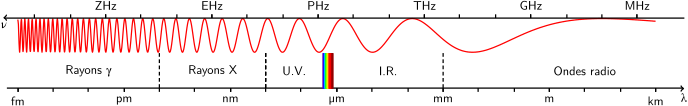
\includegraphics[scale=0.7]{Images/Spectre_Electromagnetique.png}
		\caption{Domaines du spectre électromagnétique}
	\end{center}
\end{figure}
Le domaine \emph{optique} est la réunion du domaine du visible et de l'infrarouge (I.R.).
Bien que les satellites puissent embarquer aussi d'autres types de capteurs, nous n'en parlerons pas, car cela n'a pas de rapport avec l'Imagerie Satellite.

Par ailleurs, nous nous focaliserons uniquement sur les capteurs passifs, c'est-à-dire des capteurs qui ne font que mesurer le rayonnement d'un objet, contrairement aux capteurs actifs, comme les radars qui émettent un rayonnement et en observent l'écho sur l'objet.
\subsubsection{Capteurs de type Whisk Broom}
Ce sont les premiers capteurs historiques utilisés pour l'imagerie satellite, utilisés par exemple dès $1970$ sur les satellites du programme LANDSAT de la NASA.

Le fonctionnement de ce type de capteur s'apparente au mécanisme des premiers scanners, c'est à dire une unique cellule de détection, qui nécessitait un double balayage selon les axes des lignes et des colonnes pour décrire la scène.
En anglais, le terme \emph{whisk broom} désigne des balais à \emph{fouetter}, comme par exemple des plumeaux.

Voici un schéma décrivant le fonctionnement d'un capteur de type \emph{whisk broom} :
\begin{figure}[H]
	\begin{center}
		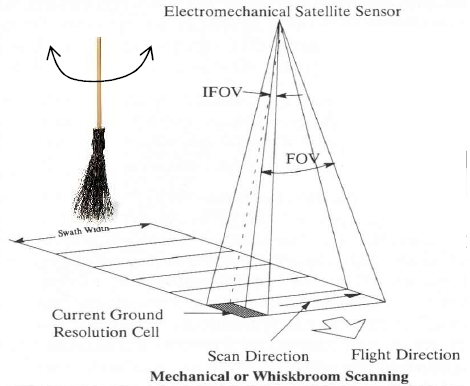
\includegraphics[scale=1.]{Images/Whisk_Broom.jpg}
		\caption{Capteur de type \emph{Whisk Broom}}
	\end{center}
\end{figure}
Les avantages d'un capteur \emph{whisk broom} sont les suivants :
\begin{itemize}
	\item Étant donné qu'un seul capteur est utilisé, l'étalonnage de l'appareil est facile, permettant ainsi un rendu homogène de l'image.
	\item La fauchée, c'est-à-dire la largeur au sol de l'image, peut être très large.
\end{itemize}
Ce type de capteur présente aussi des inconvénients :
\begin{itemize}
	\item Le balayage mécanique est complexe à mettre en œuvre, au niveau des mécanismes à utiliser pour compenser les oscillations du satellite. L'usure de tels mécanismes limitent la durée de vie utile du satellite.
	\item Le temps d'intégration, c'est-à-dire le temps d'acquisition requis pour effectuer une mesure, est le fruit d'un compromis entre une bonne qualité radiométrique et la résolution au sol. En effet, pour obtenir une mesure de qualité, on préfère faire une moyenne sur un grand nombre d'acquisitions, limité par la vitesse orbitale du satellite et l'amplitude des oscillations du capteur, impactant directement la largeur de la fauchée.
\end{itemize}
\subsubsection{Capteurs de type Push Broom}
Le fonctionnement de ces capteurs est inspiré des scanners et photocopieurs grand-public apparus dans les années $1980$.

Le premier satellite équipé d'un tel dispositif était SPOT $1$, un satellite conçu par le CNES en $1986$.
Le principe de fonctionnement est assez simple, au lieu d'utiliser une unique cellule comme pour les capteurs \emph{whisk broom}, on utilise des lignes, aussi appelées barrettes, de cellules de détection.
Ainsi l'acquisition est simultanée pour les détecteurs composants une seule et même ligne.

Une image, composées de $m$ lignes et $n$ colonnes, est donc le résultat de $n$ acquisitions simultanées répétées à $m$ intervalles de temps suivant la trajectoire du satellite.

Voici un schéma décrivant le fonctionnement d'un capteur de type \emph{push broom} :
\begin{figure}[H]
	\begin{center}
		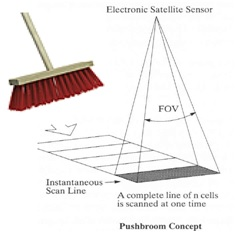
\includegraphics[scale=1.]{Images/Push_Broom.jpg}
		\caption{Capteur de type \emph{Push Broom}}
	\end{center}
\end{figure}
Les avantages d'un capteur \emph{push broom} sont les suivants :
\begin{itemize}
	\item La simplicité du système.
	\item Il ne peut y avoir des perturbations géométriques seulement le long des colonnes.
	\item Des larges fauchées grâce à la miniaturisation des cellules.
\end{itemize}
Ce type de capteur présente aussi des inconvénients :
\begin{itemize}
	\item Le plan focal, ou l'alignement, de l'ensemble des capteurs est assez difficile à réaliser.
	\item En raison du nombre important de détecteurs, l'étalonnage radiométrique de l'ensemble est assez complexe.
\end{itemize}

\subsubsection{Capteurs de type Matriciel}
Le fonctionnement de ce capteur est similaire à celui d'un appareil photographique disponible au grand public.

Les cellules de détection sont réparties en forme de grille. Ainsi tous les pixels de l'image sont acquis de façon simultanée.
Voici un schéma décrivant le fonctionnement d'un capteur de type \emph{matriciel} :
\begin{figure}[H]
	\begin{center}
		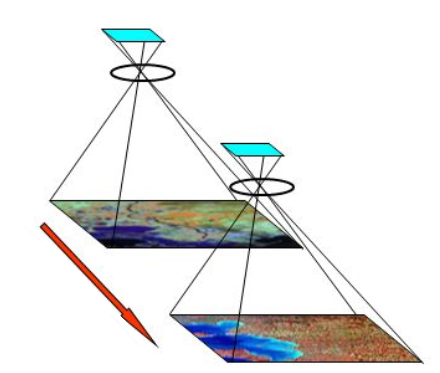
\includegraphics[scale=0.7]{Images/CCD_Sensor.png}
		\caption{Capteur de type \emph{Matriciel}}
	\end{center}
\end{figure}

Les avantages d'un capteur \emph{matriciel} sont les suivants :
\begin{itemize}
	\item Grâce à l'acquisition simultanée de tous les pixels de l'image, il ne peut y avoir de perturbations géométriques, sauf en cas de flou de bougé.
	\item La possibilité de photographier une zone selon plusieurs angles (de visée).
\end{itemize}
Ce type de capteur présente aussi des inconvénients :
\begin{itemize}
	\item L'alignement des capteurs très difficile à réaliser de par le nombre très important de détecteurs et de leur répartition en forme de matrice.
	\item L'étalonnage radiométrique délicat en raison du grand nombre de détecteurs.
	\item La difficulté d'assembler des prises de vue pour en faire des mosaïques.
\end{itemize}
\subsection{L'Orbite des Satellites}
Le mouvement d'un satellite artificiel autour de la Terre, appelé \emph{orbite}, est qualifié de képlérien car il respecte les trois lois de Kepler :
\begin{itemize}
	\item \emph{Loi des orbites} : Le satellite décrit une trajectoire elliptique, l'un des foyer de l'ellipse étant la Terre. Dans le cas présent, l'ellipse est quasi-circulaire.
	\item \emph{Loi des aires} : L'aire de la surface délimitée par la Terre et un arc $\wideparen{AB}$ de la trajectoire du satellite, noté $\wideparen{AB}T$, est égale à l'aire d'une autre surface définie par un autre arc $\wideparen{CD}$ de l'ellipse, , noté $\wideparen{CD}T$, si le temps de parcours de l'arc $\wideparen{AB}$, noté $t_{\wideparen{AB}}$, est égal à $t_{\wideparen{CD}}$.
	\item \emph{Loi des périodes} : Le carré de la période $T$ d'un satellite est proportionnel au cube du demi-grand axe $a$ de la trajectoire elliptique du satellite : $\frac{T^2}{a^3} = \frac{4 \pi^2}{\mu}$
\end{itemize}
Deux types d'orbites sont principalement utilisé pour les satellites
\subsubsection{L'Orbite Géostationnaire}
L'orbite \emph{géostationnaire} implique comme son nom l'indique que la position du satellite est fixe par rapport à la Terre.
Il faut que l'orbite du satellite soit circulaire autour de la Terre, et que la vitesse \emph{angulaire} du satellite soit égale à la vitesse \emph{angulaire} de la Terre. L'orbite se situe à environ 36000 kilomètres d'altitude.

Ce type d'orbite est utilisé pour les satellites de télécommunication, ainsi que pour des applications de surveillance de la Terre comme la météorologie, nécessitant un survol constant d'une zone définie.
\subsubsection{L'Orbite Héliosynchrone}
L'orbite \emph{héliosynchrone} signifie que le satellite est "synchronisé" avec le soleil, ce qui en d'autres termes implique que le satellite doive tourner à la même vitesse autour de la Terre que la Terre autour du Soleil.

On s'intéresse particulièrement aux orbites quasi-polaires héliosynchrones. En effet, le satellite se déplace presque selon une longitude et conserve un angle constant entre le plan d'orbite et la direction Terre-Soleil.
\begin{figure}[H]
	\begin{center}
		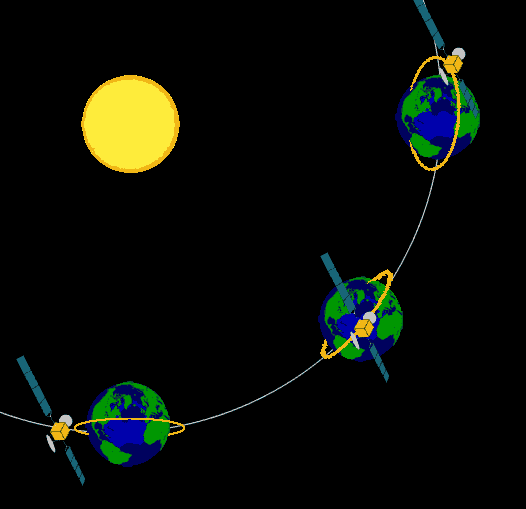
\includegraphics[scale=0.3]{Images/Orbite_Heliosynchrone.png}
		\caption{Orbite Héliosynchrone}
	\end{center}
\end{figure}
Ce type d'orbite est très intéressant pour l'imagerie spatiale car cela signifie que le satellite repasse à un point à la même heure de la journée, ce qui dans le cas d'un satellite d'observation nous permet de prendre des photographies avec une lumière ayant toujours le même angle d'incidence et donc un ensoleillement comparable.
\subsubsection{Trace au Sol et Fauchée d'un Satellite}
La trace au sol est la projection de la trajectoire décrite par un satellite à la surface du globe terrestre.

La fauchée d'un satellite est la surface au sol couverte par la prise de vue du capteur optique.
\begin{figure}[H]
	\begin{center}
		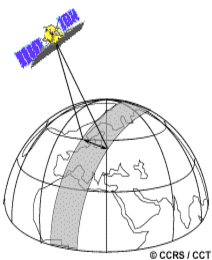
\includegraphics[scale=0.5]{Images/Swath.png}
		\caption{Fauchée d'un satellite}
	\end{center}
\end{figure}
Dans le cas d'une orbite quasi-polaire, la trace au sol recouvrira alors presque toute la surface de la Terre (sauf aux pôles), permettant de revisiter les zones de façon périodique et à la même d'heure grâce aux propriétés d'héliosynchronisme.
\begin{figure}[H]
	\begin{center}
		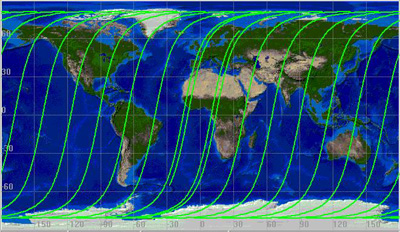
\includegraphics[scale=0.6]{Images/Trace_Sol_SPOT.jpg}
		\caption{Trace au sol des satellites SPOT sur 24h}
	\end{center}
\end{figure}
\section{Images Satellite}
Après avoir détaillé les différents types de capteurs optiques et différentes orbites utilisées pour les satellites, nous allons à présent développer un peu plus en détail le produit, les \emph{images satellite}.

\subsection{Métadonnées}
À chaque image satellite, on associe des métadonnées, c'est-à-dire des données externes, qui ne sont pas des \emph{données images}, mais qui apportent des informations complémentaires à l'image.

Voici une liste non-exhaustive des informations habituellement contenues dans les métadonnées.
\subsubsection{Le Système de Coordonnées}
Un système de coordonnées est un référentiel permettant d'exprimer la position de points dans un espace, et par conséquent une position sur le globe terrestre.
La Terre n'offre pas de surface géométriquement régulière, de ce fait on peut la représenter de différentes manières :
\begin{itemize}
	\item Une sphère est une approximation grossière de la Terre, venant du fait que la Terre est aplatie aux pôles, ce qui est dû à sa rotation. Mais cette approximation ne suffit pas pour de la cartographie précise.
	\item Un ellipsoïde, une ellipse en trois dimensions, nous permet de modéliser cet aplatissement. C'est ce modèle qui est retenu pour la cartographie.
\end{itemize}

Le système géodésique le plus courant est WGS 84 (World Geodetic System 1984), car utilisé par le système GPS. Il définit une représentation de l'ellipsoïde terrestre, ce système est référencé en $2$ dimensions, longitude et latitude, et en $3$ dimensions en ajoutant l'altitude.

On peut aussi les exprimer en représentation plane, résultant d'une projection, parfois partielle, de l'ellipsoïde (en $3$ dimensions) sur un plan (en $2$ dimensions). On citera par exemple les projections de Mercator ou de Lambert.

Ces informations, décrivant le système de coordonnées, sont contenues dans le \emph{Well-Known Text}, qui est une chaîne de caractères structurée résumant la définition du repère géographique. En voici un exemple :

\begin{verbatim}
GEOGCS["WGS 84",
    DATUM["WGS_1984",
        SPHEROID["WGS 84",6378137,298.257223563,
            AUTHORITY["EPSG","7030"]],
        AUTHORITY["EPSG","6326"]],
    PRIMEM["Greenwich",0],
    UNIT["degree",0.0174532925199433],
    AUTHORITY["EPSG","4326"]]
\end{verbatim}

\subsubsection{Positionnement et Résolution de l'Image}
Il est indispensable d'associer à toute image satellite une position dans l'espace. Une origine, généralement le coin supérieur gauche, est définie dans le système de référencement.

À cette origine, on associe la résolution spatiale de l'image, c'est-à-dire les dimensions d'un pixel dans l'espace projeté.
Par exemple,
\begin{verbatim}
Origin = (32.503388399999999,15.548911199899999)
Pixel Size = (0.000002700000000,-0.000002700000000)
\end{verbatim}
La seconde composante de la taille d'un pixel est ici négative, car l'image à pour origine le coin supérieur gauche, le parcours de l'image se fait donc en avançant dans les longitudes (sens Ouest-Est) mais en descendant les latitudes (sens Nord-Sud).

En ajoutant à ces connaissances la dimension de l'image en pixel, nous pouvons interpoler la position des autres coins de l'image. Ce calcul d'interpolation reste une approximation car il faut prendre en compte l'angle de visée du satellite par rapport au sol.

\subsection{Compression et Formats de Fichier}
Le format de fichier, aussi appelé \emph{driver}, spécifie la façon dont les données sont écrites sur le disque de stockage.
Il existe de nombreux formats de fichiers offrant des possibilités de compression avec ou sans pertes.

Un format très utilisé dans l'imagerie spatiale est le format GeoTIFF, ou GTiff, qui est un dérivé du format TIFF. Il est très utilisé de par sa flexibilité et le nombre de méthodes de compression existantes.

On citera aussi les formats :
\begin{itemize}
	\item JPEG est le format le plus courant en photographie numérique, mais étant un format de compression avec pertes il est peu utilisé en imagerie spatiale.
	\item JPEG2000 est un format propriétaire, successeur annoncé du JPEG, il offre de grandes possibilités de compression utilisant des ondelettes (ratio de $1:50$), mais la lecture/écriture sont très lentes dues aux opérations de compression/décompression.
	\item LUM est un format utilisé par le CNES en interne sur la chaîne de traitement des images et pour des simulations, c'est un fichier de format binaire accompagné de métadonnées.
\end{itemize}
\subsection{Caractéristiques d'une Image Satellite}
Nous allons à présent voir quelques propriétés concernant les images, ainsi que certaines particularités des images satellite.
\subsubsection{Angle de visée}
Pour les appareils photographiques classiques, l'angle de visée dépend de celui qui tient l'appareil, il en est de même pour les satellites. 

L'angle de visée est variable, permettant de re-photographier une zone sans avoir à attendre une période orbitale entière, durant environ $26$ jours pour les satellites de la famille SPOT.

Cependant pour pouvoir obtenir de "belles" images, afin de pouvoir les exploiter de façon optimale il faut re-projeter l'image pour se retrouver au \emph{nadir}, le \emph{nadir} étant le vecteur normal à la surface terrestre depuis le satellite. C'est donc le vecteur opposé du \emph{zénith}.
\begin{figure}[H]
	\begin{center}
		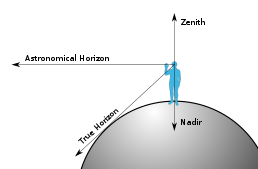
\includegraphics[scale=0.9]{Images/Nadir.png}
		\caption{Nadir, Zénith et Horizons}
	\end{center}
\end{figure}

Le fait que l'angle de visée re-projeté soit pratiquement toujours le même permet d'unifier les traitements à appliquer sur l'image et simplifier son exploitation ultérieure.
\subsubsection{Bandes et Fusion d'Images}
Une image, et en particulier une image satellite, est constituée de bandes. 

Chaque bande contient la réponse impulsionnelle de la scène sur une longueur d'onde donnée.

Voici les caractéristiques radiométriques du satellite Pléiades :
\begin{center}
	\begin{tabular}{|c|c|c|}
	\hline
	Couleur & Bande Spectrale & Résolution \\
	\hline 
	Bleu & $430$-$550$nm & $2$m \\ 
	\hline 
	Vert & $490$-$610$nm & $2$m \\ 
	\hline 
	Rouge & $600$-$720$nm & $2$m \\ 
	\hline 
	Proche Infrarouge & $750$-$950$nm & $2$m \\ 
	\hline 
	Panchromatique & $480$-$830$nm & $0.5$m \\ 
	\hline 
	\end{tabular}
\end{center}
La bande panchromatique ne discrimine pas les couleurs, son domaine de sensibilité est similaire à la vision humaine, autour de $400$-$750$nm. Ce sont des images en noir et blanc.

Comme nous pouvons le voir sur le tableau, toutes les bandes produites par le satellite Pléiades ne sont pas à la même résolution, les bandes \emph{multispectrales} sont à $2$m, tandis que la bande \emph{panchromatique} est à $0.5$m.
Pourtant le produit après traitement est composé des $4$ bandes couleurs échantillonnées à $0.5$m.

Le traitement appliqué s'appelle la fusion d'images et repose sur :
\begin{enumerate}
	\item La transformée en ondelettes de l'image \emph{panchromatique haute résolution} en une image approximée, c'est-à-dire de plus basse résolution.
	\item La substitution de l'image approximée par l'image \emph{multispectrale}.
	\item La transformée inverse en ondelettes de l'image \emph{multispectrale} pour obtenir une image \emph{multispectrale haute résolution}.
\end{enumerate}

\subsubsection{Prétraitement d'une Image Satellite}
Un grand nombre de traitements interviennent dans la correction géométrique des images afin que le produit final puisse être superposable à une carte.
Voici un récapitulatif des niveaux de traitements pour une image satellite de la famille SPOT :
\begin{itemize}
	\item Niveau 1A : Correction des défauts radiométriques issus des écarts de sensibilité entre les détecteurs élémentaires.
	\item Niveau 1B : Égalisation radiométrique et traitements géométriques relatifs aux variations d'altitude du satellite, à la rotation et à la courbure de la Terre, aux variations de l'angle de visée, etc.
	\item Niveau 2A : Projection de l'image dans le référentiel WGS $84$, la localisation d'un pixel est précise à $300$m.
	\item Niveau 2B : Correction géométriques : utilisation de points d'appuis au sol, de la modélisation de la dynamique de vol, etc.
	\item Niveau 3 : Produit appelé \emph{orthoimage}, où l'erreur de localisation est encore diminuée grâce à des modèles numériques d'élévation pour ajuster le relief, l'erreur de localisation est de $10$m pour des images ayant une résolution de $10$m.
\end{itemize}
\section{Conclusion}
Dans ce chapitre, nous avons entraperçu le domaine de l'imagerie spatiale.
Nous avons brièvement listé les différents types de capteurs optiques ainsi que deux types d'orbites utilisées pour les satellites artificiels.

Nous avons aussi détaillé différentes caractéristiques d'une image satellite, ainsi que la structure des fichiers contenant ces images.

C'est un domaine extrêmement complexe, où se mêlent des disciplines telles que la mécanique képlerienne, l'électronique ou encore le traitement d'image, et où l'erreur n'est pas tolérée.

Ce chapitre a permis au lecteur de comprendre la nature d'une image satellite, permettra de comprendre par la suite, le raisonnement employé dans le quatrième chapitre portant sur les applications pratiques.

\chapter{L'Apprentissage Machine}
L'apprentissage machine permet d'accomplir des tâches traditionnellement compliquées pour les ordinateurs, mais considérées simples pour l'humain.
En effet, l'humain apprend par exemple dès le plus jeune âge à discerner les contours sur une image, d'en décrire le contenu et même de visualiser un objet sous différents angles. Des algorithmes classiques ont du mal à produire des bons résultats sur ce genre de problèmes.
À l'inverse, les ordinateurs possèdent une capacité très supérieure à l'humain pour résoudre des calculs complexes, ou des problèmes d'ordre combinatoire.

D'un point de vue scientifique et philosophique, l'apprentissage machine est très intéressant et soulève beaucoup de questions, car l'étude de l'apprentissage appliqué aux machines nous permettrait peut-être d'entrevoir certains principes définissant l'intelligence.
\section{Définition d'un Algorithme Apprenant}
Un algorithme apprenant est un algorithme capable d'utiliser des données pour accomplir des tâches. La définition la plus célèbre, proposée par T.M Mitchell, est la suivante :
\begin{displayquote}
	On dit qu'un algorithme apprend grâce à une expérience \emph{E}, par rapport à une classe de tâches à accomplir \emph{T}, dont on peut calculer la mesure de performance (ou d'accomplissement) \emph{P}, si sa capacité d'accomplir la tâche \emph{T}, mesurée par la performance \emph{P}, s'améliore avec l'expérience \emph{E}.
\end{displayquote}

Un tel algorithme basera son apprentissage sur un jeu de données. Un jeu de données est un ensemble d'exemples.
Chaque exemple, noté $e$, est composé d'une entrée, notée $x$, à laquelle on peut associer, dans le cas d'un apprentissage supervisé, une sortie attendue, notée $\hat{y}$.
\subsection{La Tâche}
Le processus d'apprentissage ne représente pas la tâche. L'apprentissage symbolise les moyens d'acquérir la possibilité, qui peut être aussi vue comme la capacité, d'accomplir une tâche en particulier.
Par exemple, si l'on veut apprendre à un robot à lire, la tâche en question sera la capacité à lire.

En apprentissage machine, une tâche, notée \emph{T}, consiste à faire, pour chaque exemple $e$, correspondre une entrée $x$ à un résultat de sortie $y$.
Une entrée $x$ est au sens statistique un individu décrit par un ensemble de variables.
\begin{center}
	Un individu est représenté par un vecteur $x \in \mathbb{R}^n$, avec $n$ étant le nombre de variables décrivant l'individu et $x_i$ la $i$-ème variable.
\end{center}
Par exemple, une image est vue comme une matrice $I \in \mathbb{R}^{m \times n}$ de pixels, que nous pouvons projeter sur un vecteur $x \in \mathbb{R}^k$, avec $k = m \times n$.

Voici à présent un aperçu non exhaustif des tâches.
\subsubsection{Classification}
La classification consiste à déterminer, pour une entrée $x \in \mathbb{R}^n$, en sortie, une ou plusieurs parmi $k$ catégories, ou classes, associées à l'entrée.

Pour résoudre ce type de problème, l'algorithme apprenant doit produire une fonction $f : \mathbb{R}^n \in E$, avec $E$ étant un ensemble de dimension $k$.
On notera que la structure de $E$ n'est pas fixée.

On peut par exemple avoir :
\begin{itemize}
	\item $E = \{1,..,k\}$, dans ce cas, la classification est dite simple, car pour tout individu $x$ donné, il ne peut correspondre qu'une seule classe.
	\item $E = \{0,1\}^k$, dans ce cas la classification est multiple, car il peut correspondre $0$, $1$ ou plusieurs classes.
	\item $E = \{y \in [0,1]^k/ \sum_{i=1}^{k}{y_i}=1  \}$, dans ce cas, la sortie $y$ représente une distribution de probabilité.
\end{itemize}
La classification est par exemple utilisée pour la reconnaissance d'objets, l'entrée $x$ étant l'image, et la sortie $y$, la classe de l'objet dans l'image.
\subsubsection{Régression}
La régression consiste à prédire une valeur réelle en fonction d'un individu en entrée.

L'algorithme doit par conséquent se comporter comme une fonction $f : \mathbb{R}^n \rightarrow \mathbb{R}$, en faisant correspond à un individu donné $x \in \mathbb{R}^n$, une prédiction $y \in \mathbb{R}$.

On l'utilise par exemple pour l'approximation de fonctions modélisant un phénomène ou encore la prédiction des cours des actions.
\subsubsection{Autres Applications}
Les deux applications citées ci-dessus sont les plus connues et les plus largement utilisées, toutefois il en existe un grand nombre telles que :
\begin{itemize}
	\item La transcription, consistant à traduire des données sans structure particulière en données ayant une structure discrète. Par exemple, extraire le texte d'une image, ou la reconnaissance vocale.
	\item La traduction, consistant à traduire une suite de caractères d'une langue à une autre.
	\item Le débruitage, ou \emph{denoising} : Il s'agit de reconstituer à partir d'un exemple bruité $\tilde{x} \in \mathbb{R}^n$, l'original $x \in \mathbb{R}^n$, en prédisant la probabilité $p(x|\tilde{x})$, c'est à dire que $x$ soit l'original de $\tilde{x}$.
\end{itemize}
		
\subsection{La Mesure de la Performance}
Afin de quantifier les performances d'un algorithme d'apprentissage machine, il nous faut définir une mesure. Cette mesure, notée \emph{P}, est généralement spécifique à la tâche \emph{T} donnée à l'algorithme.
Pour des tâches, telles que la classification, la transcription ou la traduction, on mesure généralement la précision, c'est à dire la proportion d'exemples ou la sortie proposée par le modèle est similaire à la sortie attendue.
Néanmoins, cette mesure n'est pas générale, en effet, par exemple pour une tâche de régression, si l'écart entre la sortie produite et la sortie attendue est faible mais non nul, alors faut-il considérer le modèle comme valide ?

Pour cela, nous définissons une mesure plus générale, une \emph{fonction de perte }associée.
Cette fonction de perte n'a pas de forme particulière car elle dépend de la tâche \emph{T} à réaliser, mais elle décroît à mesure que la sortie $y$ produite par l'algorithme est "bonne".

Afin de réaliser un bon apprentissage, il nous faut donc minimiser cette \emph{fonction de perte}.

L'apprentissage machine se résume donc à optimiser notre algorithme pour modéliser au mieux une situation.
		
\subsection{L'Expérience}
On peut distinguer deux grandes classes d'algorithmes d'apprentissage machines, les algorithmes d'apprentissage \emph{non-supervisés} et \emph{supervisés}.

Une expérience \emph{E} peut être comprise comme le fait d'apprendre sur un \emph{jeu de données}.
\subsubsection{Apprentissage Non-Supervisé}
Les algorithmes d'apprentissage machine non-supervisés ont pour but d'apprendre sur des jeux de données ne contenant que des entrées $x$, et par exemple apprendre la distribution de probabilité $p(x)$ du jeu de données, ou bien de répartir les données dans des clusters, par le biais d'une distance donnée.
\subsubsection{Apprentissage Supervisé}
Les algorithmes d'apprentissage machine supervisés ont pour but d'apprendre sur un jeu de données, à associer une entrée $x$ à une sortie $y$, que l'on veut proche de la sortie attendue $\hat{y}$. Ce qui peut être vu comme l'apprentissage de la probabilité de $p(y|x)$.
	
\section{Contraintes d'Apprentissage et Régularisation}
\subsection{Sous-apprentissage, Sur-apprentissage et Capacité d'un Algorithme Apprenant}
L'un des défis majeurs en apprentissage machine est la possibilité de bien raisonner sur de nouveaux exemples encore inconnus de l'algorithme. Cette capacité de raisonnement s'appelle la généralisation.
En effet, un algorithme apprenant s'appuie pour l'entraînement sur un ensemble d'apprentissage, ce qui nous permet de mesurer l'\emph{erreur d'apprentissage}, terme équivalent à la \emph{fonction de perte} sur les données d'apprentissage, et ainsi de la minimiser.

Ce qui différencie un simple problème d'optimisation de l'apprentissage machine, est que nous souhaitons non seulement que notre algorithme ait une \emph{erreur d’apprentissage} faible, mais que sa capacité à généraliser, traduite par l'\emph{erreur de généralisation} ou \emph{erreur de test}, soit aussi petite que possible.

Ainsi, pour juger de l'efficacité d'un algorithme apprenant, nous devons prendre en compte l'\emph{erreur d'apprentissage}, mais aussi que la différence entre l'\emph{erreur d'apprentissage} et l'\emph{erreur de test}.
\subsubsection{Sous-apprentissage}
Le phénomène de sous-apprentissage survient lorsque pour un problème donné et un modèle choisi, l'\emph{erreur d'apprentissage} n'est pas suffisamment faible pour obtenir de bons résultats.
On peut donc interpréter le sous-apprentissage comme étant l'incapacité d'un modèle à ajuster un phénomène.
\subsubsection{Sur-apprentissage}
Le phénomène de sur-apprentissage survient lorsque l'écart entre l'\emph{erreur d'apprentissage} et l'\emph{erreur de test} est trop grand. Cela signifie que notre modèle, proposé par l'algorithme d'apprentissage, a été capable d'apprendre suffisamment sur les exemples d'entraînement, mais n'est pas capable de généraliser sur des exemples de test, sur lesquels il n'a pas appris.
\subsubsection{Capacité}
On peut alors définir la \emph{capacité} d'un modèle comme étant la mesure théorique de ses performances d'apprentissage mais aussi de ses performances en terme de généralisation.

Ainsi le modèle le plus adapté à notre problème aura une capacité suffisante pour apprendre correctement la fonction à produire par rapport aux données, mais ne sera pas trop grande, afin de garder un pouvoir suffisant de généralisation.
			
\subsubsection{Exemple}
Nous allons maintenant introduire un exemple nous permettant d'illustrer ces concepts.

La tâche \emph{T} est une régression polynomiale, c'est-à-dire que nous devons trouver un polynôme $P \in \mathbb{R}^{q}$ ajustant au mieux nos données.

$P$ est donc de la forme :
$$P(z) = b + \sum_{j=1}^{q}{\theta_j z^j}$$
L'expérience \emph{E} est un ensemble de $n$ points $(x_i,y_i)$, que l'on peut résumer en deux vecteurs :
$$x, y \in \mathbb{R}^n$$
Et la mesure de performance \emph{P}, le critère des moindres carrés, c'est-à-dire :
$$J_0(x,y) =\frac{1}{2} \sum_{i=1}^{n}{(P(x_i)-y_i)^2}$$
Si l'on considère que $P(x) = (P(x_i))_{i=1..q}$, alors on peut réécrire $J_0(x,y)$ tel que :
$$J_0(x,y) = \frac{1}{2} (P(x)-y)^T(P(x)-y)$$
Voici le nuage de $10$ points à ajuster :
\begin{figure}[H]
	\begin{center}
		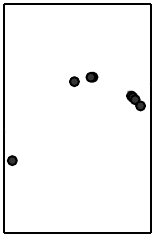
\includegraphics[scale=0.5]{Images/Fitting_Problem.png}
		\caption{Nuage de $10$ points à ajuster}		
	\end{center}
\end{figure}
			
			
Si nous choisissons un polynôme $P \in \mathbb{R}^1$, c'est à dire de la forme $P(z) = b + \theta z$, en minimisant le \emph{problème des moindres carrés}, nous obtenons la courbe suivante.
\begin{figure}[H]
	\begin{center}
		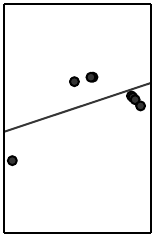
\includegraphics[scale=0.5]{Images/Underfitting.png}
		\caption{Cas de sous-apprentissage}			
	\end{center}
\end{figure}
Sans même faire d'études statistiques, on peut voir que le modèle ajuste mal les données.
Si nous choisissons par contre un polynôme $P \in \mathbb{R}^9$, en minimisant le \emph{problème des moindres carrés}, nous obtenons la courbe suivante.
\begin{figure}[H]
	\begin{center}
		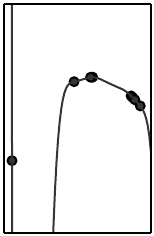
\includegraphics[scale=0.5]{Images/Overfitting.png}
		\caption{Cas de sur-apprentissage}
	\end{center}
\end{figure}
On peut s'apercevoir que même si la droite passe exactement par nos $10$ points, le modèle ne semblera pas ajuster d'éventuelles nouvelles données.
			
Enfin, si l'on choisit un polynôme $P \in \mathbb{R}^2$, nous ajustons tous les points du jeu de données et le modèle semble suffisamment simple pour généraliser de nouvelles données.
\begin{figure}[H]
	\begin{center}
		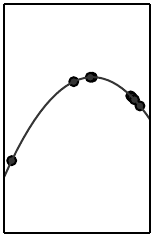
\includegraphics[scale=0.5]{Images/Good_Fitting.png}
		\caption{Capacité du modèle adaptée}
	\end{center}
\end{figure}
		
\subsection{Régularisation}
Dans l'exemple précédent, nous avons vu que le choix du modèle influait sur sa capacité, c'est à dire de tenter de produire une fonction suffisamment générale par rapport au phénomène représenté par les données.
Afin d'améliorer les capacités de généralisation des algorithmes d'apprentissage machine, un principe, dont les premières formulations sont attribuées à Ptolémée, $II^e$ siècle, connu dans la littérature, sous le nom du Rasoir d'Occam (ou Ockham) est le suivant : 
\begin{displayquote}
	Les hypothèses suffisantes les plus simples sont les plus vraisemblables.
\end{displayquote}
Ce principe de parcimonie, ou de simplicité, consiste à ne pas utiliser d'hypothèses spécifiques à un problème, si il existe des hypothèses générales plus simples répondant à ce même problème.

Ainsi pour résoudre notre problème, notre modèle doit être suffisamment performant sur un problème spécifique, mais doit être assez général pour produire des résultats corrects si l'on change quelques hypothèses.
\begin{figure}[H]
	\begin{center}
		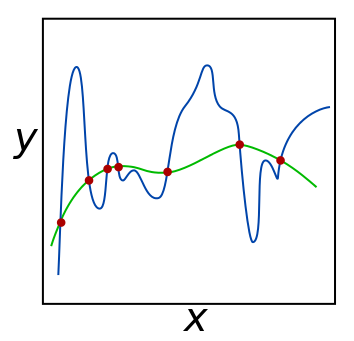
\includegraphics[scale=0.5]{Images/Regularization.png}
		\caption{Dilemme du choix entre deux modèles}
	\end{center}
\end{figure}
Dans cet exemple, nous choisirons bien entendu la courbe verte, car le modèle vert est beaucoup plus simple et nous semble plus cohérent par rapport à nos données.
Cette recherche d'un modèle optimal mais suffisamment simple peut se faire en ajoutant une composante à la mesure de performance.

En reprenant l'exemple précédent, nous pouvons ajouter à $J_0(x,y)$ une fonction $f$ arbitraire, qui aurait tendance à pénaliser l'effet de sur-apprentissage.
Cette fonction $f$ peut dépendre par exemple des coefficients $\theta_i$ du polynôme.
Ce qui nous donne une fonction :
$$J(x,y,\theta) = J_0(x,y) + \lambda f(\theta)$$
On peut choisir par exemple $f(\theta) = \sum_{i=1}^{q}{\theta_i^i}$ et ainsi pénaliser les coefficients d'ordre élevé, ainsi notre algorithme aura tendance à proposer des polynômes ayant des coefficients d'ordre élevé de petite taille, et ainsi réduire artificiellement l'ordre du polynôme choisi.

Le terme de \emph{régularisation} est employé pour toute modification apportée à l'algorithme apprenant visant à réduire l'\emph{erreur de généralisation}, mais pas l'\emph{erreur d'apprentissage}.
	
\section{Paramétrisation et Validation d'un Algorithme}
La plupart des algorithmes d'apprentissage machine sont paramétrés afin de contrôler plus précisément leur apprentissage.
Ces paramètres s'appellent des \emph{hyper-paramètres}.

Par exemple dans l'exemple de la régression polynomiale, nous avons utilisé deux \emph{hyper-paramètres} :
\begin{itemize}
	\item $q$ : le degré du polynôme $P$ utilisé.
	\item $\lambda$ : le coefficient de décroissance appliquée à la fonction $f(\theta)$.
\end{itemize}
En effet, ces deux paramètres doivent être manuellement choisis par rapport à notre problème, en fonction de notre besoin de généralisation ($\lambda$) ou de performance sur l'apprentissage ($q$).

Afin de vérifier que notre algorithme soit correctement paramétré, il nous faut construire un troisième jeu de données, appelé ensemble de validation.
Voici les propriétés de ces jeux de données.
\begin{itemize}
	\item Le premier jeu de données est l'ensemble d'apprentissage, notre algorithme apprendra donc uniquement sur cet ensemble.
	\item Le second jeu de données est l'ensemble de test, il est indépendant du premier. Nous pourrons vérifier grâce à ce jeu de données si l'algorithme est apte à généraliser.
	\item Le troisième jeu de données est l'ensemble de validation. En règle générale, on soustrait au jeu d'apprentissage une petite fraction de ses données. Grâce à lui, nous pouvons vérifier l'hyper-paramétrisation de notre algorithme.
\end{itemize}
Ainsi la procédure d'expérimentation est la suivante :
\begin{enumerate}
	\item Choix d'un modèle.
	\item Choix des hyper-paramètres.
	\item Apprentissage sur l'ensemble d'apprentissage.
	\item Estimation de la capacité de généralisation du modèle sur l'ensemble de validation.
	\item Si la capacité à généraliser est trop faible, c'est à dire que l'\emph{erreur de validation} est trop élevée, on modifie les hyper-paramètres, puis retour à l'étape d'apprentissage, sinon on passe à l'étape suivante.
	\item Évaluation finale des performances du modèle sur l'ensemble de test.
	\item Si l'\emph{erreur de test} est trop élevée, alors il faut retourner à la première étape et choisir un nouveau modèle, sinon on valide le modèle.
\end{enumerate}
	
\section{Optimisation}
Dans cette section, nous aborderons les grands principes utilisés pour réaliser l'apprentissage à proprement parler.
Nous rappelons qu'en effet le but d'un algorithme d'apprentissage machine est s'améliorer à réaliser une tâche \emph{T} grâce à une expérience \emph{E}, cette amélioration étant mesurée par \emph{P}.

Nous voulons donc ici, minimiser l'\emph{erreur d'apprentissage} afin d'améliorer nos performances sur la tâche à réaliser.
\subsection{Méthodes exactes}
Les méthodes exactes sont très pratiques, car elles permettent de trouver la solution de façon immédiate.
Pour résoudre le problème $min_{\theta}J(x,y)$, il nous faut donc annuler le gradient de la fonction de perte, soit
\begin{center}
	$\nabla_{\theta} J(x,y) = 0$
\end{center}
Cela nécessite un certain travail en amont, dépendant entièrement du type d'algorithme utilisé.

De plus il n'existe \textbf{pas toujours de solution exacte unique}.
\subsubsection{Exemple}
Prenons le cas de la régression polynomiale, le problème est le suivant :
\begin{center}
	$min_{\theta,b} J(x,y) = \frac{1}{2} (P(x)-y)^T(P(x)-y)$
	
	$\leftrightarrow$ Trouver $\theta \in \mathbb{R}^q$ et $b \in \mathbb{R}$, tels que la fonction de perte $J(x,y)$ soit minimale.
\end{center}
Pour rappel, 
\begin{center}
	$P(z) = b + \sum_{j=1}^{q}{\theta_j z^j}$,
		un polynôme de degré $q$,
		et $P(x) = (P(x_i))_{i=1..n}$,
		le polynôme d'un vecteur $P(x)$ est le vecteur de polynômes $P(x_i)$.
		Donc $P(x) = 
	\begin{pmatrix}
		1      & x_1    & \cdots & x_1^q  \\
		\vdots & \cdots & \cdots & \vdots \\
		\vdots & \cdots & \cdots & \vdots \\
		1      & x_n    & \cdots & x_n^q  
	\end{pmatrix} 
	\begin{pmatrix}
		b        \\
		\theta_1 \\
		\vdots   \\
		\theta_n 
	\end{pmatrix}
	= X \theta
	$
\end{center}
On peut alors réécrire $J(x,y)$ de la façon suivante :
\begin{center}
	$J(x,y) = \frac{1}{2} (P(x)-y)^T(P(x)-y) = \frac{1}{2} (X\theta-y)^T(X\theta-y)$
		$\rightarrow J(x,y) =\frac{1}{2} (\theta^TX^TX\theta - 2\theta^TX^Ty + y^Ty)$
\end{center}
Il nous faut maintenant trouver le minimum de $J(x,y)$, ce qui revient à résoudre $\nabla_\theta J(x,y) = 0$
Or, grâce aux dérivées vectorielles ($\frac{\partial x^Ta}{\partial x} = a$, et $\frac{\partial x^TAx}{\partial x} = 2Ax$ )
\begin{center}
	$\nabla_\theta J(x,y) = \frac{1}{2} (2X^TX\theta-2X^Ty) = X^TX\theta-X^Ty$
\end{center}
Donc,
\begin{center}
	$X^TX\theta-X^Ty = 0$
		$\rightarrow X^TX\theta = X^Ty$
		$\rightarrow \theta = (X^TX)^{-1} X^Ty$
\end{center}
Néanmoins une méthode exacte présente des inconvénients.

Par exemple, pour calculer $\theta$, la complexité algorithmique est de l'ordre de $O(n^3)$, avec $n$ le nombre de données, à cause de l'inversion de matrice.
Cette complexité cubique pose donc des problèmes quand $n$ est très grand.
De plus cette méthode présente des problèmes de stabilité numérique, si le conditionnement de $X^TX$ est grand.
		
\subsection{Méthodes itératives}
Nous avons vu dans un premier temps, que les méthodes exactes permettaient parfois avec, un peu de calcul formel, d'avoir une solution optimale à notre problème, et ce immédiatement.

Une méthode itérative, comme son nom l'indique, converge vers le résultat après plusieurs itérations.
Elles peuvent remplacer les méthodes exactes, quand celles-ci sont soit inapplicables, coûteuses ou inconnues. De plus lorsqu'un problème est mal conditionné, elles limitent la propagation des erreurs.

Il existe un grand nombre de méthodes itératives, mais nous n'en aborderons qu'une seule catégorie, car utile pour la suite, les méthodes de descente du gradient.

Les méthodes de descente de gradient, sont très utilisées en apprentissage machine, de par leur facilité d'implémentation, ainsi que de leur convergence plutôt rapide.
\subsubsection{Algorithme de Descente de Gradient}
Voici à présent l'algorithme général du gradient, appliqué à une fonction $J(x,y,\theta)$.
\begin{algorithm}[H]
	\caption{Algorithme général de Descente de Gradient}
	\begin{algorithmic}
		\REQUIRE {
			L'ensemble des entrées $x=(x_i)_{i=1}^n$ et l'ensemble des sorties $y=(y_i)_{i=1}^n$
						$x_i$ et $y_i$ sont des vecteurs réels de dimensions quelconques,
						$\theta_0$, les paramètres initiaux du modèle,
						et $\epsilon > 0$, seuil de tolérance.
		}
		\REPEAT
		\STATE Calcul de $\nabla_\theta J(x,y,\theta_k)$.
		\STATE Calcul de $\alpha_k$.
		\COMMENT{$\alpha_k$ peut être soit une constante, soit calculé en fonction de gradients $\nabla_\theta J(x,y,\theta)$}
		\STATE $\theta_{k+1} = \theta_k - \alpha_k \nabla_\theta J(x,y,\theta_k)$.
		\UNTIL{$\nabla_\theta J(x,y,\theta_k) \leq \epsilon$}
		\RETURN $\theta_{k+1}$
	\end{algorithmic}
\end{algorithm}
Dans notre cas, nous souhaitons minimiser la fonction de perte associée à notre modèle par rapport aux données d'apprentissage.

Soit $x$ et $y \in \mathbb{R}^n$, les entrées et les sorties.

On pose ici $J(x,y,\theta)$ l'erreur moyenne du modèle par rapport aux données d'apprentissage.
$$J(x,y,\theta) = \frac{1}{n} \sum_{i=1}^{n}{J(x_i,y_i,\theta)}$$
Donc,
$$\nabla_\theta J(x,y,\theta) = \frac{1}{n} \sum_{i=1}^{n}{\nabla_\theta J(x_i,y_i,\theta)}$$
\			
\subsubsection{Algorithme de Descente de Gradient Stochastique}
La réflexion derrière la descente de gradient stochastique est que le gradient de l'ensemble est la moyenne des gradients des couples $(x,y)$ .

D'après la Loi des Grands Nombres, $$\mathbb{E}(X) \approx \frac{1}{n} \sum_{i=1}^{n}{x_i}$$
Avec $X$ une distribution, dont les données $x_i$ sont issues.

Par ailleurs, si l'on échantillonne de façon uniforme $m$ individus parmi les $n$ données d'apprentissage, on aura :
$$\mathbb{E}(X) \approx \frac{1}{m} \sum_{i=1}^{m}{x_i}$$
Ainsi,
$$\frac{1}{n} \sum_{i=1}^{n}{x_i} \approx \frac{1}{m} \sum_{i=1}^{m}{x_i}$$
L'ensemble des $m$ variables extraites de $x$ s'appelle \emph{mini-lot} ou \emph{mini-batch}
\begin{algorithm}[H]
	\caption{Algorithme de Descente de Gradient Stochastique}
	\begin{algorithmic}
		\REQUIRE {
			L'ensemble des entrées $x=(x_i)_{i=1}^n$ et l'ensemble des sorties $y=(y_i)_{i=1}^n$
						$x_i$ et $y_i$ sont des vecteurs réels de dimensions quelconques,
						$m < n$,
						$\theta_0$, les paramètres initiaux du modèle, initialisés aléatoirement,
						$\alpha > 0$, le pas de descente
						et $\epsilon > 0$, seuil de tolérance.
		}
		\REPEAT
		\STATE $\hat{x},\hat{y} = sample(x,y,m)$
		\STATE Calcul de $\nabla_\theta J(\hat{x},\hat{y},\theta_k)$.
		\STATE Calcul de $\alpha_k$.
		\COMMENT{$\alpha_k$ peut être soit une constante, soit calculé en fonction de gradients $\nabla_\theta J(x,y,\theta)$}
		\STATE $\theta_{k+1} = \theta_k - \alpha_k \nabla_\theta J(\hat{x},\hat{y},\theta_k)$.
		\UNTIL{$\nabla_\theta J(\hat{x},\hat{y},\theta_k) \leq \epsilon$}
		\RETURN $\theta_{k+1}$
	\end{algorithmic}
\end{algorithm}
L'intérêt de cette méthode repose principalement sur le fait que le gradient moyen du \emph{mini-batch} est une très bonne approximation du gradient moyen calculé sur l'ensemble des données, et nous permet ainsi d'ajuster les paramètres du modèle plus souvent, permettant généralement une convergence plus rapide.

\section{Conclusion}
Ce chapitre nous a permis de poser les bases de l'apprentissage machine, sans toutefois se focaliser sur quelque algorithme apprenant.

Nous avons défini clairement la notion d'apprentissage machine, évoqué différentes contraintes liées à l'apprentissage, et expliqué les notions de validation et d'optimisation de tels algorithmes

Ce chapitre permettra au lecteur de pouvoir saisir pleinement le concept et les motivations de l'apprentissage profond évoqué dans le chapitre suivant.

\chapter{L'Apprentissage Profond}
L'apprentissage profond se différencie de l'apprentissage machine classique particulièrement sur deux points :
\begin{itemize}
	\item Il existe des dizaines, voire des centaines de classes d'algorithmes d'apprentissage pour résoudre des tâches variées, et par extension des problèmes très variés, cependant dans le cas de l'apprentissage profond, même si il existe des différences, le principe utilisé reste globalement le même.
	
	De ce fait leur capacité de généralisation est beaucoup plus forte, permettant ainsi de résoudre plus efficacement certains problèmes jugés difficiles à résoudre par des algorithmes d'apprentissage classiques.
	\item Si le principe de l'algorithme reste globalement le même, la structure du modèle est quant à elle très variable, et il est même très important de la faire varier d'un problème à un autre, car elle est intrinsèquement dépendante du problème et de ses données.
	      \end{itemize}
Nous présenterons, dans un premier temps, le fonctionnement des réseaux totalement connectés, car les plus simples. Ainsi que différentes méthodes employées pour améliorer les performances des modèles.

Dans un second temps, nous verrons une variante, les réseaux convolutifs.

Enfin, nous aborderons succinctement différentes applications existantes appliquées à la vision.
\section{Réseaux de Neurones Profonds}
Les réseaux de neurones profonds, aussi appelés \emph{Deep Feedforward Networks}, définissent un \emph{mapping} entre un vecteur d'entrée $x$ et sa sortie associée $y$ de sorte que $y = f(x,\theta)$ et apprennent les paramètres $\theta$ de sorte à produire la meilleure estimation.

Ils sont dits "\emph{feedforward}", ou en français à "propagation unique", car l'information se déplace à travers la fonction, depuis l'entrée $x$, puis par des étapes intermédiaires, pour arriver à la sortie $y$, sans aucun retour en arrière.

Les réseaux de neurones permettant un \emph{feedback} ou \emph{retour d'expérience} font partie de la classe des réseaux récurrents.
Les réseaux de types "\emph{feedforward}" sont de loin les réseaux de neurones les plus utilisés.

On utilise le mot \emph{réseau} dans l’appellation réseaux de neurones, car ils sont composés d'une multitude de fonctions \emph{simples}, organisées en réseau.

On pourrait par exemple imaginer notre fonction $f(x,\theta)$ comme étant la composée de plusieurs fonctions, telle que $f(x,\theta) = u_{\theta_1} \circ v_{\theta_2} \circ w_{\theta_3}(x)$ avec $\theta = (\theta_1,\theta_2, \theta_3))$, un ensemble de paramètres.
C'est par ailleurs cette architecture distribuée, qui grâce à une puissance de calcul grandissante, par le biais du calcul GPU, permet de résoudre des problèmes de plus en plus complexes.
\subsection{Définition d'un Neurone Artificiel}
Ce que l'on appelle \emph{neurone} est effectivement inspiré du fonctionnement d'un neurone biologique, bien que différent à bien des égards.

Un neurone artificiel est une application $f : \mathbb{R}^p \rightarrow \mathbb{R}$, paramétrée par $\theta = (b,w) = (b, w_1, ..., w_p)$.

Le réel $b$ s'appelle le biais, et le vecteur $w = (w_1, ..., w_p)$ s'appelle vecteur de poids.
\begin{figure}[H]
	\begin{center}
		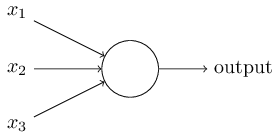
\includegraphics[scale=0.6]{Images/Neuron.png}
		\caption{Schéma de représentation d'un Neurone}
	\end{center}
\end{figure}
Cette application est la composée de deux fonctions distinctes :
\begin{itemize}
	\item Une fonction d’\emph{agrégation} $h : \mathbb{R}^p \rightarrow \mathbb{R}$, combinant l'entrée $x$ avec les poids $w$ et le biais $b$.
	      	      Dans le cas d'un neurone \emph{totalement connecté} (le plus basique), elle à l'allure suivante :
	      $$h_\theta(x) = h_{b,w}(x) = w^Tx + b = \sum_{i=1}^{p}{w_i x_i} + b$$
	\item Une fonction d'\emph{activation} $g : \mathbb{R} \rightarrow \mathbb{R}$, \emph{non-linéaire}.
	      	      Des exemples :
	      \begin{itemize}
	      	\item \emph{ReLU}, pour \emph{Rectified Linear Unit} : $g(z) = max(0,z)$
	      	\item \emph{Sigmoïde} : $g(z) = \frac{1}{1+e^{-z}}$
	      	\item \emph{Tangente hyperbolique} : $g(z) = \tanh(z)$
	      \end{itemize}
\end{itemize}
Il est important de garder à l'esprit que ces deux opérations successives sont distinctes, mais qu'elles sont regroupées ici pour montrer les similarités avec les neurones biologiques.

Ainsi notre neurone peut être résumé par une fonction $f$ telle que :
$$f_\theta(x) = g \circ h_\theta(x) = g(w^Tx + b)$$
La sortie de notre neurone, par la suite notée $a$, est l'\emph{image} de la fonction $f$ par l'entrée $x$:
$$a = f_\theta(x) = g \circ h_\theta(x) = g(w^Tx + b)$$
\subsection{Définition d'un Réseau de Neurones}
Avec la définition précédente d'un neurone, nous pouvons alors schématiser un réseau de neurones de la façon suivante :
\begin{figure}[H]
	\begin{center}
		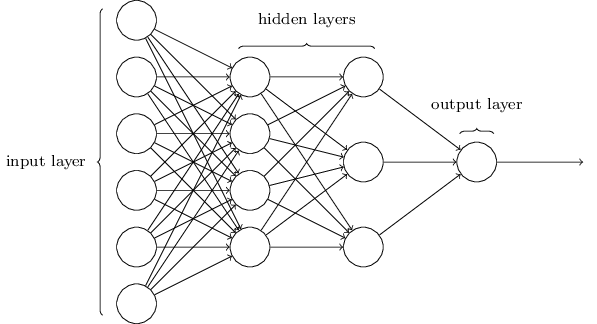
\includegraphics[scale=0.6]{Images/Neural_Network.png}
		\caption{Schéma pédagogique de représentation d'un Réseau de Neurones}
	\end{center}
\end{figure}
Ici, chaque cercle représente un neurone, équivalent à ceux définis précédemment.
Toutefois, sur la première couche, appelée \emph{couche d'entrée}, les neurones produisent en sortie, le \emph{vecteur d'entrée} $x$, ici $x \in \mathbb{R}^6$.
On peut noter aussi que la dernière couche, appelée \emph{couche de sortie}, les neurones produisent le vecteur $y$, ici $y\in \mathbb{R}^1 = \mathbb{R}$.

Attention, la description faite ici, n'est qu'à but pédagogique. Dans le cas courant, on ne considère pas un réseau en individualisant chaque neurone, mais plutôt couche par couche :
\begin{figure}[H]
	\begin{center}
		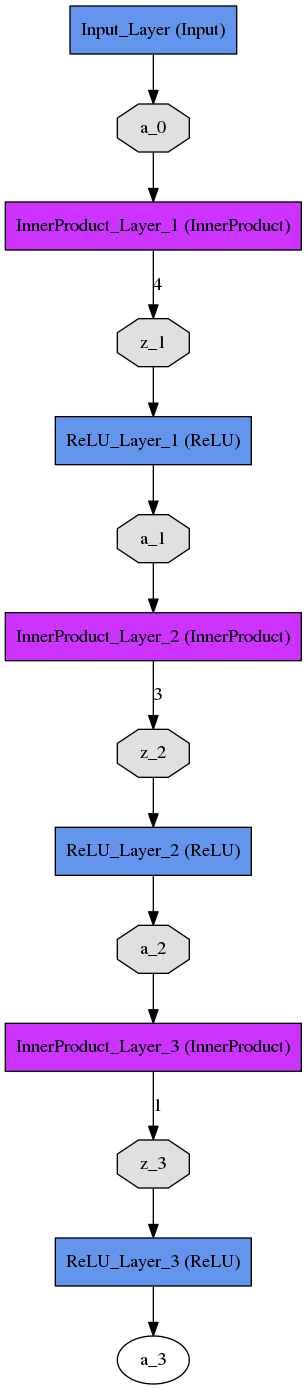
\includegraphics[scale=0.4]{Images/Toy_Example.png}
		\caption{Schéma courant de représentation d'un Réseau de Neurones}
	\end{center}
\end{figure}

Ainsi, pour décrire un réseau de neurones, nous considérons deux caractéristiques :
\subsubsection{Profondeur}
\begin{center}
	Le nombre de couches d'un réseau de neurones est appelé \emph{profondeur}, plus ce nombre est élevé, plus la capacité théorique de généralisation est forte.
\end{center}
Même si il n'existe pas de seuil officiel différenciant les réseaux de neurones, \emph{peu profonds}, dits \emph{superficiels}, des réseaux de neurones \emph{profonds}, on parle d'\emph{apprentissage profond} lorsque le nombre de couches cachées est $\geq 2$.
On parlera d'apprentissage très profond, lorsque le nombre de couches cachées est $\geq 10$.
\subsubsection{Largeur}
\begin{center}
	Le nombre de neurones composant une couche est appelé \emph{largeur}.
	\end{center}
Nous pouvons par ailleurs noter que le nombre de paramètres $\theta = (b,w) = (b,w_1,..,w_p)$ d'un neurone n'est pas arbitraire.
En effet, la \emph{largeur} de chaque couche est égale au nombre de paramètres $\theta$ des neurones de la couche suivante.
Par ailleurs, la \emph{largeur} de la première couche est égale à la taille du vecteur d'entrée $x$.
\subsubsection{Expression Générale}
On explicitera généralement l'architecture d'un réseau de neurones par un vecteur $s \in \mathbb{N}^L$.
Ainsi $S = (S_1, S_2, ..., S_L)$ représente un réseau de neurones de \emph{profondeur} $L$ ($L$ couches), chacune possédant $s_i$ neurones ayant $s_{i-1}$ poids et un biais par neurone.
\subsection{Notations}
Afin de ne pas se perdre dans les calculs qui vont survenir, nous allons définir une notation nous permettant de repérer sans ambiguïté la position des différents éléments d'un réseau de neurones.
\begin{center}
	\emph{\textbf{Important !}}
\end{center}
Chaque élément du réseau de neurones peut être défini par sa position dans le réseau.\\
Pour les \emph{poids} :
\begin{itemize}
	\item Un poids \emph{réel} noté $\elem{W}{k}{j}{i}$ sera le $i$-ème poids du $j$-ème neurone, situé dans la $k$-ème couche.
	\item Par conséquent $\elem{W}{k}{j}{}$ sera quant à lui le vecteur de poids du $j$-ème neurone, situé dans la $k$-ème couche.
	\item Enfin $\elem{W}{k}{}{}$ sera la matrice des poids de la $k$-ème couche.
	      \end{itemize}
Pour les \emph{biais} :
\begin{itemize}
	\item Un biais \emph{réel} noté $\elem{b}{k}{j}{}$ sera le biais du $j$-ème neurone, situé dans la $k$-ème couche.
	\item Par conséquent $\elem{b}{k}{}{}$ sera quant à lui le vecteur de biais de la $k$-ème couche.
	      \end{itemize}
Nous noterons par ailleurs avec la lettre $a$, qui sera indicée par la suite, la sortie d'une couche du réseau.
Pour les \emph{sorties} :
\begin{itemize}
	\item Une sortie d'un neurone noté $\elem{a}{k}{j}{}$ sera la sortie du $j$-ème neurone, situé dans la $k$-ème couche.
	\item Par conséquent $\elem{a}{k}{}{}$ représente le vecteur de sortie de la $k$-ème couche, mais aussi le vecteur d'entrée de la $(k+1)$-ème couche.
	\item Le vecteur d'entrée $x$, sera noté $\elem{a}{0}{}{}$.
	\item Le vecteur de sortie $y$, sera noté $\elem{a}{L}{}{}$ dans un réseau de $L$ couches.
	      \end{itemize}
Enfin, les résultats de la fonction de combinaison sont de même dimensions que les sorties de couche.
Pour les \emph{combinaisons} :
\begin{itemize}
	\item Une combinaison notée $\elem{z}{k}{j}{}$ sera la combinaison du $j$-ème neurone, situé dans la $k$-ème couche.
	\item Par conséquent $\elem{z}{k}{}{}$ représente le vecteur des combinaisons de la $k$-ème couche.
	      \end{itemize}
			
\subsection{Propagation}
On parle de \emph{propagation à sens unique} dans un réseau de neurones, car l'entrée $x$, affectée à la première couche, est transmise à la suivante, qui produira alors un vecteur de sortie.
Ce vecteur de sortie sera alors considéré comme un vecteur d'entrée pour la couche suivante, qui produira à l'aide de cette entrée un autre vecteur de sortie.
Et ainsi de suite, jusqu'à la dernière couche, qui produira finalement la sortie du réseau : $y$.
		
Nous voilà à présent correctement armés pour voir la propagation dans un réseau de neurones.
Voici l'algorithme de propagation au sein d'un réseau de neurones : 
\begin{algorithm}[H]
	\caption{Algorithme de Propagation}
	\begin{algorithmic}
		\REQUIRE {
			Un réseau de neurones de $L$ couches, défini par $S = (S_1, S_2, ..., S_L)$.
						Un vecteur d'entrée $x \in \mathbb{R}^n = \mathbb{R}^{S_1}$,
					}
		\STATE $\elem{a}{0}{}{} = x$
		\FOR{$k=1$ \TO $L$}
		\FOR{$j=1$ \TO $S_k$}
		\STATE $\elem{z}{k}{j}{} = (\elem{W}{k}{j}{})^T(\elem{a}{k-1}{}{}) + \elem{b}{k}{j}{} = \sum_{i=1}^{S_{k-1}}{\elem{W}{k}{j}{i} \times \elem{a}{k-1}{i}{}} + \elem{b}{k}{j}{}$
		\STATE $\elem{a}{k}{j}{} = g(\elem{z}{k}{j}{})$
				\COMMENT{$\elem{a}{k}{j}{}$ est, comme vu précédemment, la sortie du $j$-ème neurone de la $k$-ème couche,
						$\elem{z}{k}{j}{}$ est le résultat de la fonction d'agrégation, résultat très utile par la suite.
			$\elem{W}{k}{j}{}$ est le vecteur de poids du $j$-ème neurone de la $k$-ème couche,
						et $\elem{b}{k}{j}{}$ est le biais du $j$-ème neurone de la $k$-ème couche.}
		\ENDFOR
		\ENDFOR
		\RETURN $\elem{a}{L}{}{}$
		\COMMENT{$\elem{a}{L}{}{}$ est la sortie du réseau de neurones, que nous comparerons ensuite à $y$.}
	\end{algorithmic}
\end{algorithm}
			
Néanmoins, il existe aujourd'hui un grand nombre de bibliothèques permettant de faire du calcul matriciel de façon optimisée, appelées Basic Linear Algebra Subprograms (BLAS), telles que ATLAS, GotoBLAS, OpenBLAS.

Pour rappel, $\elem{W}{k}{}{}$ représente la matrice des poids de la $k$-ème couche, et $\elem{a}{k-1}{}{}$ le vecteur de sortie de la $(k-1)$-ème couche.
Par conséquent, on peut calculer le vecteur de sortie de la $k$-ème couche de la façon suivante :
$$\elem{z}{k}{}{} = (\elem{W}{k}{}{})^T(\elem{a}{k-1}{}{}) + \elem{b}{k}{}{}$$
$$\elem{a}{k}{}{} = g(\elem{z}{k}{}{})$$
Ainsi,
\begin{algorithm}[H]
	\caption{Algorithme matriciel de Propagation}
	\begin{algorithmic}
		\REQUIRE {
			Un réseau de neurones de $L$ couches, défini par $S = (S_1, S_2, ..., S_L)$.
						Un vecteur d'entrée $x \in \mathbb{R}^n = \mathbb{R}^{S_1}$,
					}
		\STATE $\elem{a}{0}{}{} = x$
		\FOR{$k=1$ \TO $L$}
		\STATE $\elem{z}{k}{}{} = (\elem{W}{k}{}{})^T(\elem{a}{k-1}{}{}) + \elem{b}{k}{}{}$
		\STATE $\elem{a}{k}{}{} = g(\elem{z}{k}{}{})$
		\ENDFOR
		\RETURN $\elem{a}{L}{}{}$
	\end{algorithmic}
\end{algorithm}
			
\subsection{Rétro-propagation du Gradient}
		
L'algorithme de rétro-propagation est souvent à tort considéré comme étant la méthode d'optimisation utilisée pour minimiser la fonction de perte.
C'est en effet le rôle d'une méthode de descente de gradient.

Voici pour rappel une méthode générale de descente de gradient, vue dans la première partie :
\begin{algorithm}[H]
	\caption{Algorithme général de Descente de Gradient}
	\begin{algorithmic}
		\REQUIRE {
			$x$ et $y \in \mathbb{R}^n$,
						$\theta_0$, les paramètres initiaux du modèle,
						et $\epsilon > 0$, seuil de tolérance.
		}
		\REPEAT
		\STATE Calcul de $\nabla_\theta J(x,y,\theta_k)$.
		\STATE Calcul de $\alpha_k$.
		\COMMENT{$\alpha_k$ peut être soit une constante, soit calculé en fonction de gradients $\nabla_\theta J(x,y,\theta)$}
		\STATE $\theta_{k+1} = \theta_k - \alpha_k \nabla_\theta J(x,y,\theta_k)$.
		\UNTIL{$\nabla_\theta J(x,y,\theta_k) \leq \epsilon$}
		\RETURN $\theta_{k+1}$
	\end{algorithmic}
\end{algorithm}
L'algorithme de rétro-propagation du gradient a pour simple but de calculer, de façon élégante, le gradient $\nabla_\theta J(x,y,\theta)$, avec $\theta$ représentant ici tous les paramètres du modèle, c'est à dire l'ensemble des poids $\elem{W}{k}{j}{i}$ et des biais $\elem{b}{k}{j}{}$.
		
\subsubsection{Calcul Formel du Gradient}
			
Il nous faut donc calculer $\frac{\partial J(x,y,\theta)}{\partial \elem{W}{k}{j}{i}}$, traduisant l'influence du poids $\elem{W}{k}{j}{i}$ sur la fonction de perte $J(x,y,\theta)$.

Et $\frac{\partial J(x,y,\theta)}{\partial \elem{b}{k}{j}{}}$, qui traduit l'influence du biais $\elem{b}{k}{j}{}$ sur la fonction de perte $J(x,y,\theta)$.
\begin{center}
	\textbf{Toute dérivée partielle $\frac{\partial u}{\partial v}$ représente l'influence qu'a l'élément $v$ sur l'élément $u$.}
\end{center}
Nous utiliserons le Théorème de dérivation des fonctions composées, aussi appelée \emph{chain rule}.
Nous rappelons que $J(x,y,\theta)$ est une fonction de perte de la forme :
$$J(x,y,\theta) = C(\elem{a}{L}{}{}(x),y)$$
				
\emph{Afin de mieux comprendre la preuve, on peut s'aider d'un \textbf{dessin \smiley{}}.}
				
\paragraph{Calcul sur la Couche de Sortie}
				
Commençons par calculer le gradient de l'erreur pour les poids de la couche de sortie, $\frac{\partial C}{\partial \elem{W}{L}{j}{i}}$.
Ainsi que le gradient pour les biais de la couche de sortie, $\frac{\partial C}{\partial \elem{b}{L}{j}{}}$.

Sur la dernière couche, nous avons
$$\elem{z}{L}{j}{} = (\elem{W}{L}{j}{})^T(\elem{a}{L-1}{}{}) + \elem{b}{L}{j}{}$$
Et
$$\elem{a}{L}{j}{} = g(\elem{z}{L}{j}{})$$
Utilisons à présent la règle de chaînage sur $\frac{\partial C}{\partial \elem{W}{L}{j}{i}}$, car $\elem{a}{L}{j}{}$ est une fonction composée.

Nous obtenons donc,
$$\left\{
\begin{array}{l}
	\frac{\partial C}{\partial \elem{W}{L}{j}{i}} = \frac{\partial C}{\partial \elem{a}{L}{j}{}} \times \frac{\partial \elem{a}{L}{j}{}}{\partial \elem{z}{L}{j}{}} \times \frac{\partial \elem{z}{L}{j}{}}{\partial \elem{W}{L}{j}{i}} 
	\\                                                                                                                                                                                                                                
	                                                                                                                                                                                                                                    
	\frac{\partial C}{\partial \elem{b}{L}{j}{}} = \frac{\partial C}{\partial \elem{a}{L}{j}{}} \times \frac{\partial \elem{a}{L}{j}{}}{\partial \elem{z}{L}{j}{}} \times \frac{\partial \elem{z}{L}{j}{}}{\partial \elem{b}{L}{j}{}}   
	\\                                                                                                                                                                                                                                
\end{array}
\right.$$
				
On s'aperçoit ici que le terme $\frac{\partial C}{\partial \elem{a}{L}{j}{}}$, exprime la variation de $C(\elem{a}{L}{}{}(x),y)$ en fonction de la sortie du neurone $\elem{a}{L}{j}{}$.
				
On voit aussi que le terme $\frac{\partial \elem{a}{L}{j}{}}{\partial \elem{z}{L}{j}{}}$, traduit la variation de la sortie du neurone $\elem{a}{L}{j}{}$ en fonction de l'agrégat $\elem{z}{L}{j}{}$, dépend de la \emph{fonction d'activation} choisie.
				
Nous reviendrons sur les expressions de $\frac{\partial C}{\partial \elem{a}{L}{j}{}}$ et $\frac{\partial \elem{a}{L}{j}{}}{\partial \elem{z}{L}{j}{}}$, car elles nous permettront de choisir de façon éclairée la fonction d'activation et la fonction coût,car des simplifications peuvent s'opérer.
				
Enfin $\frac{\partial \elem{z}{L}{j}{}}{\partial \elem{W}{L}{j}{i}}=\elem{a}{L-1}{i}{}$ et $\frac{\partial \elem{z}{L}{j}{}}{\partial \elem{b}{L}{j}{i}} = 1$, ce qui est évident à vérifier, car 
$$\elem{z}{L}{j}{} = \sum_{i=1}^{S_{L-1}}{\elem{W}{L}{j}{i} \times \elem{a}{L-1}{i}{}} + \elem{b}{L}{j}{}$$
				
Ces deux expressions traduisent l'influence des poids $\elem{W}{L}{j}{i}$ et du biais $\elem{b}{L}{j}{}$ sur l'agrégat, ou résultat de la fonction d'agrégation, $\elem{z}{L}{j}{}$
				
Pour la suite, nous allons poser $\elem{\delta}{L}{j}{} = \frac{\partial C}{\partial \elem{a}{L}{j}{}} \times \frac{\partial \elem{a}{L}{j}{}}{\partial \elem{z}{L}{j}{}}$, cela interviendra quand nous montrerons le caractère récursif de la rétro-propagation.
				
Finalement, nous obtenons,
$$\left\{
\begin{array}{l}
	\frac{\partial C}{\partial \elem{W}{L}{j}{i}} = \elem{\delta}{L}{j}{} \times \frac{\partial \elem{z}{L}{j}{}}{\partial \elem{W}{L}{j}{i}} = \elem{\delta}{L}{j}{} \times \elem{a}{L-1}{i}{} 
	\par                                                                                                                                                                                        
	                                                                                                                                                                                            
	\frac{\partial C}{\partial \elem{b}{L}{j}{}} = \elem{\delta}{L}{j}{} \times \frac{\partial \elem{z}{L}{j}{}}{\partial \elem{b}{L}{j}{}} = \elem{\delta}{L}{j}{}                             
	\par                                                                                                                                                                                        
\end{array}
\right.$$
Avec,
$$\elem{\delta}{L}{j}{} = \frac{\partial C}{\partial \elem{a}{L}{j}{}} \times \frac{\partial \elem{a}{L}{j}{}}{\partial \elem{z}{L}{j}{}}$$
				
\paragraph{Calcul sur l'avant dernière couche}
				
Après avoir explicité les calculs des $\frac{\partial C}{\partial \elem{W}{L}{j}{i}}$ et $\frac{\partial C}{\partial \elem{b}{L}{j}{}}$, passons à présent au calcul sur l'avant dernière couche, soit aux $\frac{\partial C}{\partial \elem{W}{L-1}{j}{i}}$ et $\frac{\partial C}{\partial \elem{b}{L-1}{j}{}}$.

Grâce à la \emph{chain rule}, nous obtenons de la même façon que précédemment,
				
$$\left\{
\begin{array}{l}
	\frac{\partial C}{\partial \elem{W}{L-1}{j}{i}} = \frac{\partial C}{\partial \elem{a}{L-1}{j}{}} \times \frac{\partial \elem{a}{L-1}{j}{}}{\partial \elem{z}{L-1}{j}{}} \times \frac{\partial \elem{z}{L-1}{j}{}}{\partial \elem{W}{L-1}{j}{i}} 
	\\                                                                                                                                                                                                                                            
	\frac{\partial C}{\partial \elem{b}{L-1}{j}{}} = \frac{\partial C}{\partial \elem{a}{L-1}{j}{}} \times \frac{\partial \elem{a}{L-1}{j}{}}{\partial \elem{z}{L-1}{j}{}} \times \frac{\partial \elem{z}{L-1}{j}{}}{\partial \elem{b}{L-1}{j}{}}   
	\\                                                                                                                                                                                                                                            
\end{array}
\right.$$
				
On peut remarquer que l'utilisation de la \emph{Chain rule} permet d'exprimer facilement $\frac{\partial \elem{a}{L-1}{j}{}}{\partial \elem{z}{L-1}{j}{}}$, $\frac{\partial \elem{z}{L-1}{j}{}}{\partial \elem{W}{L-1}{j}{i}}$ et $\frac{\partial \elem{z}{L-1}{j}{}}{\partial \elem{b}{L-1}{j}{}}$.
En effet si la fonction d'activation reste la même pour tout le réseau de neurones, alors le terme $\frac{\partial \elem{a}{L-1}{j}{}}{\partial \elem{z}{L-1}{j}{}}$ est la même que $\frac{\partial \elem{a}{L}{j}{}}{\partial \elem{z}{L}{j}{}}$ calculée plus haut.

De même que précédemment $\frac{\partial \elem{z}{L-1}{j}{}}{\partial \elem{W}{L-1}{j}{i}}=\elem{a}{L-2}{i}{}$ et $\frac{\partial \elem{z}{L-1}{j}{}}{\partial \elem{b}{L-1}{j}{i}} = 1$, car
$$\elem{z}{L-1}{j}{} = \sum_{i=1}^{S_{L-2}}{\elem{W}{L-1}{j}{i} \times \elem{a}{L-2}{i}{}} + \elem{b}{L-1}{j}{}$$
				
La difficulté réside ici, dans le calcul de $\frac{\partial C}{\partial \elem{a}{L-1}{j}{}}$.
Si on trace un réseau de neurones quelconque.

Prenons le $j$-ème neurone de la couche $L-1$, on peut voir qu'il transmet le résultat de son activation $\elem{a}{L-1}{j}{}$ à tous les neurones de la couche $L$.

Cette diffusion d'informations a aussi un impact sur le coût, puisque si erreur il y a alors, les neurones de la couche $L$ en feront les "frais".

Un neurone $\elem{a}{L-1}{i}{}$ propage l'erreur à un neurone $\elem{a}{L}{j}{}$ proportionnellement au poids $\elem{W}{L}{j}{i}$.
				
Nous devons donc décomposer $\frac{\partial C}{\partial \elem{a}{L-1}{j}{}}$, grâce à la \emph{chain rule}.
				
Le résultat est le suivant :	
$$\frac{\partial C}{\partial \elem{a}{L-1}{j}{}} = \sum_{l=1}^{L-1}{\frac{\partial C}{\partial \elem{a}{L}{l}{}} \times \frac{\partial \elem{a}{L}{l}{}}{\partial \elem{z}{L}{l}{}} \times \frac{\partial \elem{z}{L}{l}{}}{\partial \elem{a}{L-1}{l}{}}}$$
En effet, le neurone $\elem{a}{L-1}{i}{}$ transfère son erreur à tous les neurones $\elem{a}{L}{j}{}$ de la couche suivante par le biais des poids, car $\frac{\partial \elem{z}{L}{l}{}}{\partial \elem{a}{L-1}{j}{}} = \elem{W}{L-1}{l}{j}$.

On remarque par ailleurs que 
$$\frac{\partial C}{\partial \elem{a}{L-1}{j}{}} = \sum_{l=1}^{L-1}{\elem{\delta}{L}{l}{} \times \frac{\partial \elem{z}{L}{l}{}}{\partial \elem{a}{L-1}{j}{}}}$$
Car $$\elem{\delta}{L}{j}{} = \frac{\partial C}{\partial \elem{a}{L}{j}{}} \times \frac{\partial \elem{a}{L}{j}{}}{\partial \elem{z}{L}{j}{}}$$
Donc,
$$\elem{\delta}{L-1}{j}{} = \frac{\partial C}{\partial \elem{a}{L-1}{j}{}}  \times \frac{\partial \elem{a}{L-1}{j}{}}{\partial \elem{z}{L-1}{j}{}} = \sum_{l=1}^{L-1}{\elem{\delta}{L}{l}{} \times \frac{\partial \elem{z}{L}{l}{}}{\partial \elem{a}{L-1}{j}{}}} \times \frac{\partial \elem{a}{L-1}{j}{}}{\partial \elem{z}{L-1}{j}{}}$$
				
\paragraph{Récapitulatif}
Récapitulons, afin de voir se dessiner un schéma de récurrence.
Sur la couche $L$,
$$\left\{
\begin{array}{l}
	\frac{\partial C}{\partial \elem{W}{L}{j}{i}} = \elem{\delta}{L}{j}{} \times \frac{\partial \elem{z}{L}{j}{}}{\partial \elem{W}{L}{j}{i}} = \elem{\delta}{L}{j}{} \times \elem{a}{L-1}{i}{} 
	\\                                                                                                                                                                                        
	                                                                                                                                                                                            
	\frac{\partial C}{\partial \elem{b}{L}{j}{}} = \elem{\delta}{L}{j}{} \times \frac{\partial \elem{z}{L}{j}{}}{\partial \elem{b}{L}{j}{}} = \elem{\delta}{L}{j}{}                             
	\\                                                                                                                                                                                        
\end{array}
\right.$$
Avec,
$$\elem{\delta}{L}{j}{} = \frac{\partial C}{\partial \elem{a}{L}{j}{}} \times \frac{\partial \elem{a}{L}{j}{}}{\partial \elem{z}{L-1}{j}{}}$$
Sur la couche $L-1$,
$$\left\{
\begin{array}{l}
	\frac{\partial C}{\partial \elem{W}{L-1}{j}{i}} = \elem{\delta}{L-1}{j}{} \times \frac{\partial \elem{z}{L-1}{j}{}}{\partial \elem{W}{L-1}{j}{i}} = \elem{\delta}{L-1}{j}{} \times \elem{a}{L-2}{i}{} 
	\\                                                                                                                                                                                                  
	\frac{\partial C}{\partial \elem{b}{L-1}{j}{}} = \elem{\delta}{L-1}{j}{} \times \frac{\partial \elem{z}{L-1}{j}{}}{\partial \elem{b}{L-1}{j}{}} = \elem{\delta}{L-1}{j}{}                             
	\\                                                                                                                                                                                                  
\end{array}
\right.$$
Avec,
$$\elem{\delta}{L-1}{j}{} = \sum_{l=1}^{L-1}{\elem{\delta}{L}{l}{} \times \frac{\partial \elem{z}{L}{l}{}}{\partial \elem{a}{L-1}{j}{}}} \times \frac{\partial \elem{a}{L-1}{j}{}}{\partial \elem{z}{L-1}{j}{}}$$
\paragraph{Calcul généralisé}
Essayons à présent d'exprimer une forme récurrente applicable à chaque couche.
On a $\forall k = 1..L$,
$$\left\{
\begin{array}{l}
	\frac{\partial C}{\partial \elem{W}{k}{j}{i}} = \elem{\delta}{k}{j}{} \times \frac{\partial \elem{z}{k}{j}{}}{\partial \elem{W}{k}{j}{i}} = \elem{\delta}{k}{j}{} \times \elem{a}{k-1}{i}{} 
	\\                                                                                                                                                                                        
	\frac{\partial C}{\partial \elem{b}{k}{j}{}} = \elem{\delta}{k}{j}{} \times \frac{\partial \elem{z}{k}{j}{}}{\partial \elem{b}{k}{j}{}} = \elem{\delta}{k}{j}{}                             
	\\                                                                                                                                                                                        
\end{array}
\right.$$
Avec $$\elem{\delta}{k}{j}{} = \left\{
\begin{array}{l}
	\frac{\partial C}{\partial \elem{a}{L-1}{j}{}}, \  si \ k=L                                                                                                                                                  
	\\                                                                                                                                                                                                         
	\sum_{l=1}^{k-1}{\elem{\delta}{k+1}{l}{} \times \frac{\partial \elem{z}{k+1}{l}{}}{\partial \elem{a}{k}{j}{}} \times \frac{\partial \elem{a}{k}{j}{}}{\partial \elem{z}{k}{j}{}}}, \ si \ k \in \{1 .. L-1\}
	\\
\end{array}
\right.$$
				
Ce qui nous permet d'exprimer l'algorithme de rétro-propagation de la façon suivante :
\begin{algorithm}[H]
	\caption{Algorithme de Rétro-propagation}
	\begin{algorithmic}
		\REQUIRE {
			Un réseau de neurones de $L$ couches, défini par $S = (S_1, S_2, ..., S_L)$.
						Un vecteur d'entrée $x \in \mathbb{R}^n = \mathbb{R}^{S_1}$,
						Un vecteur de sortie $y \in \mathbb{R}^m = \mathbb{R}^{S_L}$,
					}
		\STATE
		\COMMENT{Calcul du gradient sur la couche de sortie.}
		\FOR{$j = 1$ \TO $L-1$}
		\STATE $\elem{\delta}{L}{j}{} = \frac{\partial C}{\partial \elem{a}{L-1}{j}{}}$
		\STATE $\frac{\partial C}{\partial \elem{b}{L}{j}{}} = \elem{\delta}{L}{j}{}$
		\FOR{$i =1$ \TO $L$}
		\STATE $\frac{\partial C}{\partial \elem{W}{L}{j}{i}} = \elem{\delta}{L}{j}{} \times \elem{a}{L-1}{i}{}$
		\ENDFOR
		\ENDFOR
						    
		\FOR{$k=L-1$ \TO $1$}
		\STATE
		\COMMENT{Calcul du gradient sur la $k$-ème couche.}
		\FOR{$j = 1$ \TO $k-1$}
		\STATE $\elem{\delta}{k}{j}{} = \sum_{l=1}^{k-1}{\elem{\delta}{k+1}{l}{} \times \frac{\partial \elem{z}{k+1}{l}{}}{\partial \elem{a}{k}{j}{}} \times \frac{\partial \elem{a}{k}{j}{}}{\partial \elem{z}{k}{j}{}}}$
		\STATE $\frac{\partial C}{\partial \elem{b}{k}{j}{}} = \elem{\delta}{k}{j}{}$
		\FOR{$i =1$ \TO $k$}
		\STATE $\frac{\partial C}{\partial \elem{W}{k}{j}{i}} = \elem{\delta}{k}{j}{}  \times \elem{a}{k-1}{i}{}$
		\ENDFOR
		\ENDFOR
		\ENDFOR
						    
	\end{algorithmic}
\end{algorithm}
Cet algorithme nous permet donc de calculer de façon très efficace tous les $\frac{\partial C}{\partial \elem{W}{k}{j}{i}}$ et $\frac{\partial C}{\partial \elem{b}{k}{j}{}}$.
Il existe une version privilégiant le calcul matriciel, permettant un calcul plus rapide, grâce à des librairies de BLAS.

Nous ne redémontrerons pas l'algorithme, mais nous en donneront toutefois la formulation.
\begin{algorithm}[H]
	\caption{Algorithme de Rétro-propagation Matriciel}
	\begin{algorithmic}
		\REQUIRE {
			Un réseau de neurones de $L$ couches, défini par $S = (S_1, S_2, ..., S_L)$.
						Un vecteur d'entrée $x \in \mathbb{R}^n = \mathbb{R}^{S_1}$,
						Un vecteur de sortie $y \in \mathbb{R}^m = \mathbb{R}^{S_L}$,
					}
		\STATE
		\COMMENT{Calcul du gradient sur la couche de sortie.}
		\STATE $\elem{\delta}{L}{}{} = \nabla_{\elem{a}{L-1}{}{}} C$
		\STATE $\nabla_{\elem{b}{L}{}{}} C = \elem{\delta}{L}{}{}$
		\STATE $\nabla_{\elem{W}{L}{}{}} C = \elem{\delta}{L}{}{} \times{\elem{a}{L-1}{}{}}^T $
					    
		\FOR{$k=L-1$ \TO $1$}
		\STATE
		\COMMENT{Calcul du gradient sur la $k$-ème couche.}
		\STATE $\elem{\delta}{k}{}{} = ((\nabla_{\elem{a}{k}{}{}}\elem{z}{k+1}{}{})^T \times \elem{\delta}{k+1}{}{}) \odot \nabla_{\elem{z}{k}{}{}}{\elem{a}{k}{}{}}$
		\STATE $\nabla_{\elem{b}{k}{}{}} C = \elem{\delta}{k}{}{}$
		\STATE $\nabla_{\elem{W}{k}{}{}} C = \elem{\delta}{k}{}{} \times{\elem{a}{k-1}{}{}}^T $
		\ENDFOR
	\end{algorithmic}
\end{algorithm}
Nous implémenterons alors cette méthode, car plus rapide en machine.
Nous disposons à présent des éléments suivants :
\begin{itemize}
	\item Une méthode de descente de gradient.
	\item L'algorithme de rétro-propagation, permettant le calcul du gradient de la fonction de perte de manière efficace.
\end{itemize}
Ainsi, nous disposons alors des éléments permettant de créer un réseau de neurones, ainsi que d'effectuer son apprentissage.

Nous allons maintenant quitter cette partie plutôt calculatoire, pour s'intéresser aux différents moyens existants pour améliorer les capacités de généralisation de nos futurs réseaux de neurones.
\subsection{Théorème d'Approximation Universelle}
Les réseaux de neurones permettent de représenter universellement n'importe quelle fonction, dans le sens où il existe un réseau de neurones, ayant une architecture donnée, des poids et biais donnés, pouvant approximer une fonction en particulier.

Le \emph{Théorème d'Approximation Universelle} nous dit qu'il existe un réseau suffisamment "grand" pour avoir la précision souhaitée sur les résultats.

Toutefois, ce théorème ne dit pas quelle sera la taille de ce réseau, mais en affirme seulement l'existence.
\subsection{Techniques de Régularisation}
Un défi majeur en apprentissage machine est de choisir un algorithme qui aura de bons résultats,non seulement à l'apprentissage, mais aussi sur de nouvelles entrées.
Les stratégies utilisées en apprentissage machine, permettant de réduire l'\emph{erreur de test}, parfois aux dépends de l'\emph{erreur d'apprentissage}, sont appelées techniques de régularisation.

Nous avons, dans le premier chapitre, vu les concepts généraux de la \emph{généralisation}, du \emph{sous-apprentissage} et du \emph{sur-apprentissage}.
Nous verrons à présent des méthodes concrètes appliquées aux réseaux de neurones profonds.

Certaines méthodes ajouteront des contraintes d'optimisation sur la fonction de perte, d'autres des restrictions sur les paramètres.
Si les méthodes sont choisies avec soin, elles peuvent améliorer grandement la performance des réseaux de neurones profonds sur l'ensemble des données de test.
\subsubsection{Pénalisation des Paramètres}
La pénalisation des paramètres est une des premières formes de régularisation, utilisée depuis les débuts de l'apprentissage machine.
Cette régularisation limite la capacité de modèles, tels que les réseaux de neurones, les régressions linéaires, polynomiales et logistiques, en ajoutant une composante de pénalisation des paramètres $\Omega(\theta)$ à la fonction de perte $J(x,y,\theta)$, tel que
$$J(x,y,\theta) = J_0(x,y,\theta) + \lambda \Omega(\theta)$$
Avec $\lambda \geq 0$, un hyper-paramètre pondérant la contribution de la composante de pénalisation.
Si $\lambda = 0$, il n'y a pas de régularisation.
Nous ajouterons par ailleurs que cette pénalisation n'affecte que les poids $\elem{W}{k}{j}{i}$ et non les biais $\elem{b}{k}{j}{}$, car les biais requièrent moins de données pour ajuster précisément les données.
\paragraph{Régularisation $L^2$}
Soit $w$, l'ensemble des poids du modèle,
On pose, $$\Omega(\theta) = \Omega(w) = \frac{1}{2} ||w||_2^2 = \frac{1}{2} w^T w$$
La fonction de perte s'écrit donc,
$$\tilde{J}(x,y,\theta) = J(x,y,\theta) + \frac{\lambda}{2} w^T w$$
Par conséquent le gradient s'écrit de la façon suivante,
$$\nabla_\theta \tilde{J}(x,y,\theta) = \nabla_\theta J(x,y,\theta) + \lambda w$$
Ainsi le poids $\elem{W}{k}{j}{i}$ aura tendance à diminuer par rapport à une fraction de lui même.
\subsubsection{Augmentation du Jeu de Données}
Une des meilleures façons d'améliorer la capacité de généralisation d'un modèle, est de l'entraîner sur plus de données.
Malheureusement, la taille des ensembles de données est généralement limitée.
Une façon de contourner le problème est de créer artificiellement des données et de les ajouter à l'ensemble d'apprentissage.

Cette méthode est principalement utilisée pour un domaine : la reconnaissance d'objets.
En effet, il est très facile de transformer les données existantes par des transformations, telles que des rotations, des translations ou des homothéties, paramétrées aléatoirement.
On peut aussi le faire sur d'autres types de données en ajoutant du \emph{bruit blanc} sur une partie des entrées.
\subsubsection{Arrêt Prématuré}
Pour un modèle avec une capacité suffisante pour sur-apprendre, on observe généralement que tandis que l'\emph{erreur d'apprentissage} continue de diminuer, l'\emph{erreur d'entraînement} recommence à augmenter.
Cela signifie que nous avons atteint un \emph{minimum local} sur les données de test, il convient alors d'arrêter l'apprentissage avant que l'\emph{erreur de généralisation} empire.
\subsubsection{Dropout}
La méthode \emph{Dropout} est une méthode assez particulière de régularisation, qui consiste à entraîner tour à tour des sous-réseaux de notre réseaux de neurones.
\begin{figure}[H]
	\begin{center}
		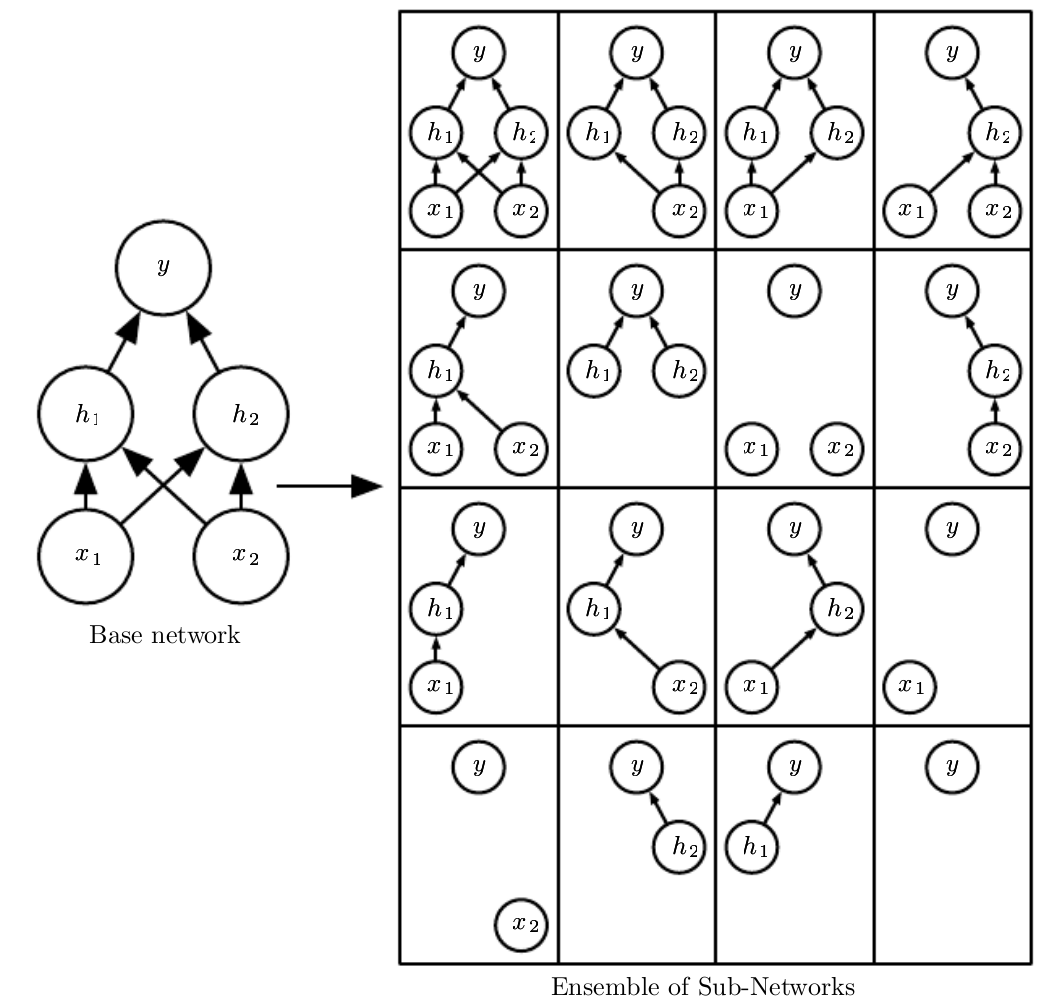
\includegraphics[scale=0.20]{Images/Dropout.png}
		\caption{Exemple d'application de la méthode de \emph{Dropout}}
	\end{center}
\end{figure}
Ainsi les différents sous-modèles se partagent les paramètres $\theta$ du modèle original.
Il en résulte un modèle beaucoup plus robuste, car les différents sous-modèles entraînent une recherche de paramètres pour atteindre des minima différents.

Cela incite donc à une convergence vers un minimum local partagé par les différents sous-modèles.
Ce minimum local est de façon générale un bien meilleur minimum que ceux propres aux sous-modèles.
Cette méthode présente toutefois un inconvénient, elle est difficile à implémenter, mais est présente dans la plupart des librairies d'apprentissage profond.
\section{Réseaux Convolutifs}
Les réseaux de neurones convolutifs sont une famille particulière de réseaux de neurones, qui excelle en terme de performance dans le domaine de la vision par ordinateur.
Ils sont spécialisés dans le traitement de données ayant une structure en forme de grille, c'est à dire que les données sont liées spatialement ou temporellement.

Voici des exemples de données ayant ce genre de structure :
\begin{itemize}
	\item Les séries temporelles pouvant être vues comme une grille de dimension $1$, car assimilables à des signaux, ayant pour unité un intervalle de temps fixe.
	\item Les images, pouvant être considérées comme étant des grilles de dimensions $2$ de pixels.
\end{itemize}
Dans un premier temps, nous définirons rapidement l'opérateur de convolution.
Dans un second temps, nous discuterons de l'intérêt des convolutions dans les réseaux de neurones, ainsi que des différences existantes entre la convolution au sens mathématique et celle employée pour l'apprentissage profond.
Enfin nous parlerons d'une opération très souvent complémentaire à celle de \emph{convolution}, appelée \emph{pooling}.
\subsection{L'Opérateur de Convolution}
L'opérateur de convolution est un opérateur bilinéaire, c'est-à-dire linéaire par rapport à chacune des opérandes, et commutatif, généralement noté $*$.

En traitement du signal, cet opérateur représente l’interaction entre un filtre et un signal.
Elle peut être vue comme une moyenne mobile d'un signal pondérée par une fonction appelée \emph{noyau}.
\subsubsection{Cas Continu}
Le produit de convolution de deux fonctions réelles ou complexes $f$ et $g$ est défini tel que,
$$(f * g)(x) = \int_{-\infty}^{+\infty}{f(x-t)g(t)dt} = \int_{-\infty}^{+\infty}{f(t)g(x-t)dt}$$
\subsubsection{Cas Discret}
Le produit de convolution de deux suites $f$ et $g$ est défini tel que,
$$(f *g)(n) = \sum_{m = -\infty}^{+\infty}{f(n-m)g(m)} = \sum_{m = -\infty}^{+\infty}{f(m)g(n-m)}$$
\subsubsection{Application aux Images}
On rappelle qu'une image $I$ de $M$ lignes et $N$ colonnes est décrite par une fonction discrète $I(i,j)$ à support fini $S \subset \mathbb{Z}^2$ et à valeurs dans $\mathbb{R}$ ou $\mathbb{N}$.
Puisque l'image, décrite par la fonction $I$ est nulle en dehors du support, on peut réécrire le produit de convolution entre des bornes finies.

Le produit de convolution en un point $(i,j)$ de deux images $I$ et $K$, noté $I * K$ est défini tel que,
On choisira d'imiter la notation matricielle pour plus de clarté.
$$(I*K)_{i,j} = \sum_{m}\sum_{n}{I_{m,n}K_{i-m,j-n}} = (K*I)_{i,j} = \sum_{m}\sum_{n}{K_{m,n}I_{i-m,j-n}}$$
L'image $K$ est appelée \emph{noyau}, ou \emph{kernel}, c'est l'équivalent d'un filtre pour les images.
Voici un exemple d'application de la convolution sur une image :
\begin{figure}[H]
	\begin{center}
		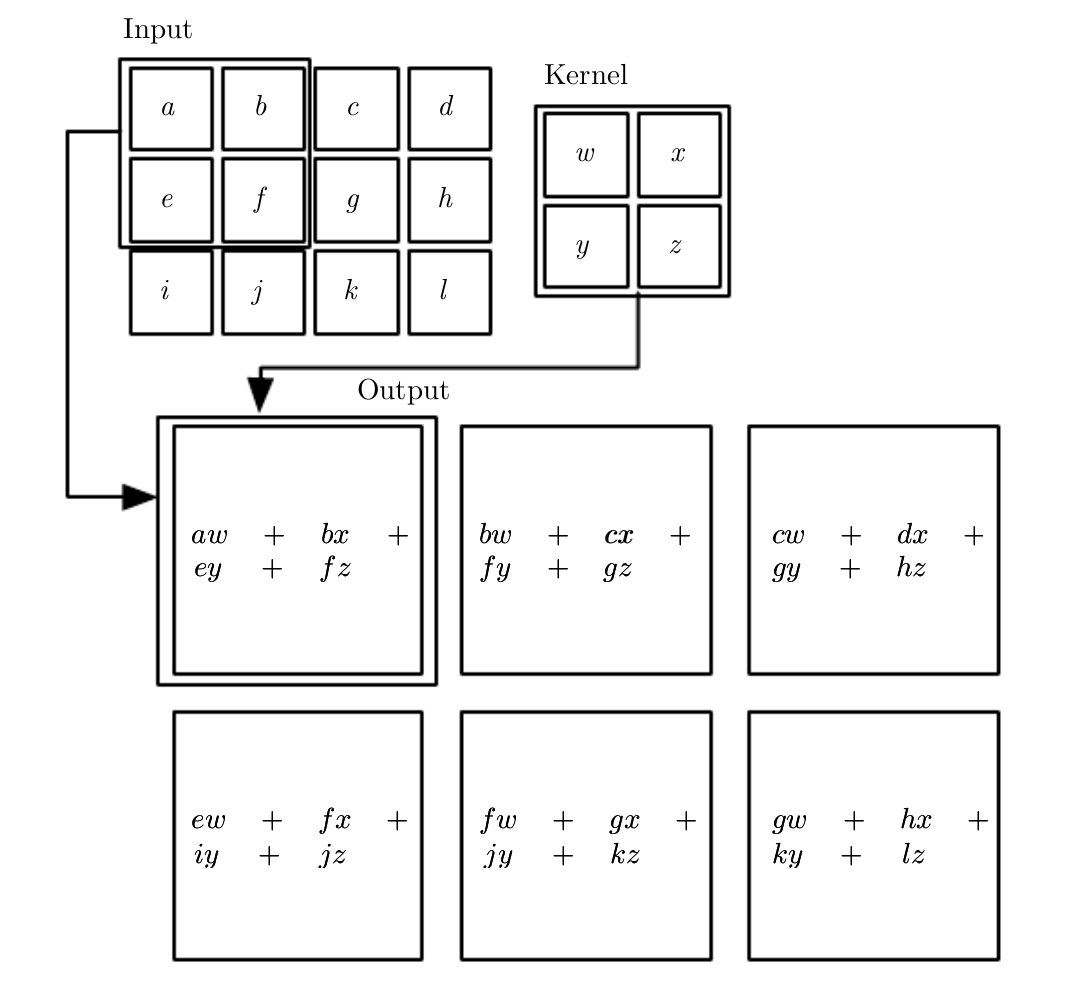
\includegraphics[scale=0.25]{Images/Convolution.png}
		\caption{Exemple de convolution entre une image $I$, $(8,3)$ et un noyau $K$, $(2,2)$}
	\end{center}
\end{figure}
Dans cet exemple de convolution entre une image $I$, $(8,3)$ et un noyau $K$, $(2,2)$, on peut remarquer tout d'abord, que l'image issue de la convolution est de forme $(6,2)$.

En effet la convolution sans \emph{padding} réduit la taille de la fenêtre.
Si l'image $I$ est de taille $(m,n)$ et le noyau de taille $(k,l)$ alors l'image convolutée sera de taille $(m-k+1,n-l+1)$.
\subsubsection{Convolution et Corrélation Croisée}
Nous avons défini précédemment la convolution entre deux images, ici une \emph{map de features} $I$ et un noyau $K$.

Nous parlerons ici de façon plus générale de convolution entre tenseurs.
\begin{center}
	Un \emph{tenseur} est un \emph{tableau multi-dimensionnel}.
	
	L'\emph{ordre} d'un tenseur est égal à la dimension du tableau.
\end{center}
Par exemple, une image en couleurs (RGB) de $256 \times 256$ pixels peut être décrite par un tenseur d'ordre $3$.
Nous écrirons alors que la dimension de l'image est $3 \times 256 \times 256$, ou bien encore $256 \times 256 \times 3$.

Toutefois, d'un point de vue machine, nous indexons celle variant le plus lentement en premier et celle variant le plus rapidement en dernier. Nous retiendrons ici l'écriture $3 \times 256 \times 256$.

Nous avons défini précédemment la convolution entre deux tenseurs d'ordre $2$, ici une \emph{map de features} $I$ et un noyau $K$, de la façon suivante :
$$(K*I)_{i,j} = \sum_{m}\sum_{n}{K_{m,n}I_{i-m,j-n}}$$
qui est équivalente à 
$$(I*K)_{i,j} = \sum_{m}\sum_{n}{I_{m,n}K_{i-m,j-n}}$$
Mais dans la pratique, le noyau $K$ étant beaucoup plus "\emph{petit}" que $I$, la première formule est préférable, au niveau du calcul des bornes des indices $m$ et $n$.
Par conséquent, même si la propriété de commutativité existe, une seule expression de la convolution nous intéresse.

La corrélation croisée, très proche de la convolution, s'écrit de la façon suivante:
$$(K*I)_{i,j} = \sum_{m}\sum_{n}{K_{m,n}I_{i+m,j+n}}$$
La différence étant par rapport au sens de l'indexation. Cette opération n'est pas commutative contrairement à la convolution, mais étant donnée que seule l'opération $K*I$ nous intéresse, cette propriété ne nous apporte rien.

Il est à noter que dans beaucoup de librairies d'Apprentissage Machine, l'opération de convolution est implémentée en tant que corrélation croisée. Dans la suite, nous appellerons convolution les deux opérations sans distinction.
			
\subsection{Intérêts de la Convolution dans les Réseaux de Neurones}
La convolution s'appuie sur trois idées importantes permettant l'amélioration des performances, l'\emph{interaction partielle}, le \emph{partage des paramètres} et l'\emph{invariance par translation}.
\subsubsection{L'interaction Partielle}
Dans les réseaux de neurones traditionnels, le passage de l'information d'une couche à la suivante se fait par la multiplication matricielle du vecteur d'entrée $\elem{a}{k-1}{}{}$ de dimension $m$, par la matrice $\elem{W}{k}{}{}$ de dimension $m \times n$, la sortie du neurone $\elem{a}{k-1}{}{}$ sera donc de dimension $n$.

Pour rappel :
$$\elem{z}{k}{}{} = (\elem{W}{k}{}{})^T(\elem{a}{k-1}{}{}) + \elem{b}{k}{}{}$$
On voit donc qu'ici l'interaction, ou connectivité, est totale puisque toutes les entrées $\elem{a}{k-1}{j}{}$ sont connectées par les poids $\elem{W}{k}{j}{i}$ aux sorties $\elem{a}{k-1}{i}{}$.
Dans le cas où l'on travaille avec des images, on peut se demander si pour un pixel donné l'information apportée par un pixel situé à l'extrême opposé de l'image est pertinente.

Ainsi, envisager une connectivité partielle entre le vecteur d'entrée $\elem{a}{k-1}{}{}$ et le vecteur de sortie $\elem{a}{k-1}{}{}$ peut sembler intéressante si l'information apportée s'apparente à du bruit.
La convolution nous permet en effet cette interaction partielle, en effet la dimension du noyau $\elem{W}{k}{}{}$, de la forme $k \times n$, et si $k < m$ alors l'interaction sera en effet partielle.

Voici à présent la représentation de l'interaction partielle dans un cas matriciel, plus illustratif qu'un simple cas vectoriel:
\begin{figure}[H]
	\begin{center}
		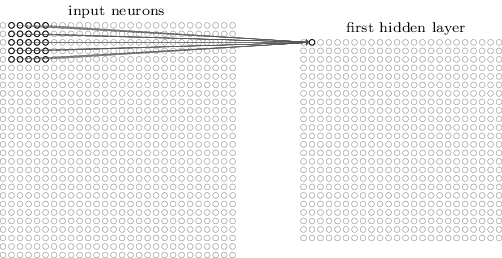
\includegraphics[scale=0.60]{Images/Convolution_Layer.png}
		\caption{Représentation de l'interaction partielle}
	\end{center}
\end{figure}
			
\subsubsection{Le Partage des Paramètres et Invariance}
Dans un réseau convolutif, chaque paramètre du noyau est utilisé à toutes les positions du vecteur d'entrée, sauf peut-être pour les premiers et derniers éléments du vecteur d'entrée.
Ainsi le partage de paramètres pour la convolution signifie qu'au lieu d'apprendre pour chaque élément du vecteur d'entrée un paramètre associé, un filtre unique, \emph{composé d'un petit nombre de paramètre}, sera appris en rapport au vecteur d'entrée.

Dans le cas de la figure précédente, où la fenêtre est de dimension $5 \times 5$, un seul noyau de dimension $5 \times 5$ sera appris pour cette couche de convolution.
Ce partage de paramètres permet alors à notre couche de convolution d'être invariante par translation.
En effet supposons que le noyau de notre couche soit entraîné à détecter un motif, ou \emph{feature} en particulier sur une image. Le noyau unique, et donc partagé à toutes les sous-régions de l'entrée, pourra détecter le motif peu importe sa position dans l'image.
			
Cette propriété d'invariance par translation rend les couches de convolutions très intéressantes, car elles sont plus robustes au bruit que des couches entièrement connectées.
				
\subsection{La Convolution appliquée aux Réseaux de Neurones}
Le terme \emph{convolution} employé dans le contexte de l'apprentissage profond, diffère quelque peu de la convolution mathématique définie comme ci-dessus.

Tout d'abord, quand on parle d'une convolution dans le contexte des réseaux de neurones, il s'agit en fait de plusieurs convolutions menées en parallèle.

Énumérons à présent les différents noyaux $K$ de convolutions, en fonction de $I$ le tenseur d'entrée et de $S$ le tenseur de sortie souhaité:
\begin{enumerate}
	\item Soient $I$ de dimensions $(H_I,W_I)$ et $S$ de dimensions $(H_S, W_S)$,\\
	Et si $H_I > H_S + 1$ et $W_I > W_S + 1$,\\
	Alors $K$ sera de dimensions :
	$$(H_K, H_K) = (H_I - H_S + 1, W_I - W_S + 1)$$
	Cette convolution nous permet d'extraire seulement une seule \emph{feature} depuis chaque sous-région de $I$.\\
	\item Soient $I$ de dimensions $(H_I,W_I)$ et $S$ de dimensions $(C_S, H_S, W_S)$,\\
	Et si $H_I > H_S + 1$ et $W_I > W_S + 1$,\\
	Alors $K$ sera de dimensions :
	$$(C_K^{out}, H_K, W_K) = (C_S, H_I - H_S + 1, W_I - W_S + 1)$$
	Cette convolution nous permet d'extraire $C_S$ \emph{features} depuis chaque sous-région de $I$.\\
	\item Soient $I$ de dimensions $(C_I, H_I,W_I)$ et $S$ de dimensions $(C_S, H_S, W_S)$,\\
	Et si $H_I > H_S + 1$ et $W_I > W_S + 1$,\\
	Alors $K$ sera de dimensions :
	$$(C_K^{out}, C_K^{in}, H_K, W_K) = (C_S, C_I, H_I - H_S + 1, W_I - W_S + 1)$$
	Cette convolution nous permet d'extraire $C_S$ \emph{features} croisées entre les $C_I$ \emph{canaux} de chaque sous-région de $I$.\\	
\end{enumerate}

Cette dernière expression est l'expression générale de la convolution.
On peut remarquer pour le premier cas, que $(H_I,W_I) = (1, H_I,W_I)$, $(H_S,W_S) = (1, H_S,W_S)$ et $(H_I,W_I) = (1, 1,  H_I,W_I)$

\subsubsection{Convolution tensorielle}
Soient $I$ de dimensions $(C_I, H_I,W_I)$ et $S$ de dimensions $(C_S, H_S, W_S)$,\\
Et si $H_I > H_S + 1$ et $W_I > W_S + 1$,\\
Alors $K$ sera de dimensions :
$$(C_K^{out}, C_K^{in}, H_K, W_K) = (C_S, C_I, H_I - H_S + 1, W_I - W_S + 1)$$

Donc $\forall k \in [0, C_S[, \ \forall i \in [0, H_S[, \ \forall j \in [0, W_S[$,
$$S(k,i,j) = \sum_{l}\sum_{m}\sum_{n}{K_{k,l,m,n} \times I_{l,m + i, n + j}}$$

Avec les indices de sommations suivants,
\begin{itemize}
	\item $l \in [\![0, C_K^{in}[\![$
	\item $m \in [\![0, H_K[\![$ et $(m + i) \in [\![0, H_I[\![$
	\item $n \in [\![0, W_K[\![$ et $(n + j) \in [\![0, W_I[\![$
\end{itemize}
\subsubsection{Padding et Strides}
\paragraph{Padding}
Nous avons pu observer précédemment que la convolution ne préservait pas les dimensions spatiales, la hauteur et la largeur, entre le tenseur d'entrée $I$ et le tenseur de sortie $S$.

Soit $I$ un tenseur de dimensions $(H_I, W_I)$ et $K$ un noyau de dimensions $(H_K, W_K)$, alors $S$ aura les dimensions suivantes :
$$(H_S, W_S) = (H_I - H_K + 1, W_I - W_K + 1)$$
Toutefois il peut être intéressant dans certains cas de préserver ces dimensions.

Le \emph{padding}, signifiant \emph{rembourrage}, permet de remédier à ce problème. Cette méthode consiste à créer un tenseur $I'$, en ajoutant à $I$ des lignes et colonnes de zéros sur ses \emph{bords}.

Ainsi, $$(H_{I'}, W_{I'}) = (H_I + p_H, W_I + p_W)$$
Donc si on applique la convolution à $I'$,
$$(H_S, W_S) = (H_I + p_H - H_K + 1, W_I + p_W - W_K + 1)$$
Donc,
$$(H_S, W_S) = (H_I, W_I) \leftrightarrow (p_H, p_W) = (H_K - 1, W_K - 1) $$

Dans le cas où les dimensions du noyau sont impaires, le \emph{padding} se fera de façon symétrique autour de $I$.
Dans le cas où les dimensions du noyau sont paires, le \emph{padding} est par convention pour les bords \emph{haut} et \emph{gauche} de $I$.

\subparagraph{Exemple}
Dans le cas d'une convolution de noyau $K$ de dimensions $(3, 3)$ appliquée à un tenseur $I$ de dimensions $(3,3)$, si on veut garder $S$ de même dimensions que $I$.

Soit
$$I =
\begin{pmatrix}
a & b & c \\ 
d & e & f \\ 
g & h & i
\end{pmatrix}$$
Alors $(p_H,p_W) = (2, 2)$\\
Donc $$I'=
\begin{pmatrix}
0 & 0 & 0 & 0 & 0\\
0 & a & b & c & 0\\ 
0 & d & e & f & 0\\ 
0 & g & h & i & 0\\
0 & 0 & 0 & 0 & 0
\end{pmatrix}
$$
\paragraph{Strides}
Le terme anglais \emph{stride} peut être traduit en français par le \emph{pas de déplacement}.\\
Augmenter le pas de déplacement dans une convolution à pour effet de diminuer la dimension du tenseur de sortie $S$.

Nous n'allons pas ici expliciter l'impact de ce changement sur les effets de l'apprentissage, un lien sera fait dans la partie dédiée au \emph{Pooling}, mais simplement décrire les modifications sur la sortie.
$$(H_S, W_S) = ((H_I - H_K) / s_H + 1, (W_I - W_K) / s_W + 1)$$
Les divisions sont ici \emph{entières} car les dimensions de sorties sont forcément entières.
\subsubsection{Convolution généralisée}
Soient $I$ de dimensions $(C_I, H_I,W_I)$,

$S$ de dimensions $(C_S, H_S, W_S)$,

$K$ de dimensions $(C_K^{out}, C_K^{in}, H_K, W_K)$, avec $C_K^{out} = C_S$ et $C_K^{in} = C_I$.

Il nous faut alors trouver $(p_H, p_W)$ et $(s_H, s_W)$, tels que :
$$(C_S, H_S, W_S) = (C_S, (H_I + p_H - H_K) / s_H + 1, (W_I + p_W - W_K) / s_W + 1)$$
On pose alors $I'$ le tenseur "\emph{rembourré}" de $I$, avec 
$$(C_{I'}, H_{I'}, W_{I'}) = (C_I, H_I + p_H, W_I + p_W)$$
Donc,
$$(C_S, H_S, W_S) = ((H_{I'} - H_K) / s_H + 1, (W_{I'} - W_K) / s_W + 1)$$
Donc $\forall k \in [0, C_S[, \ \forall i \in [0, H_S[, \ \forall j \in [0, W_S[$,
$$S(k, i, j) = \sum_{l}\sum_{m}\sum_{n}{K_{k, l, m, n} \times {I'}_{l, m + i \times s_H, n + j \times s_W}}$$
Avec,
\begin{itemize}
	\item $l \in [\![0, C_K^{in}[\![$
	\item $m \in [\![0, H_K[\![$ et $(m + i \times s_H) \in [\![0, H_{I'}[\![$
	\item $n \in [\![0, W_K[\![$ et $(n + j \times s_W) \in [\![0, W_{I'}[\![$
\end{itemize}
\subsection{La Réduction de la Dimensionnalité}
La \emph{réduction de la dimensionnalité} est un défi majeur en Statistiques et en Apprentissage Machine.

Prenons un exemple pour illustrer le problème.
Imaginons que nous souhaitons classifier des images issues d'Internet de dimensions $(3,256,256)$, en $1000$ classes distinctes.
Ce problème revient à devoir trouver un \emph{mapping} entre un tenseur d'entrée de dimensions $(3, 256, 256)$ et un tenseur de sortie de dimension $(1000)$.

On remarque qu'on peut transformer le tenseur d'entrée en un tenseur de dimension $(3 \times 256 \times 256) = (196\ 608)$.

On peut alors se poser plusieurs questions,
\begin{itemize}
	\item Quelles sont les variables significatives parmi les $196608$ variables disponibles ?
	\item Comment \emph{transformer}, ou \emph{modeler}, cette quantité d'information pour en extraire l'essentiel, c'est à dire sa classe ?
\end{itemize}

Tout d'abord la première question n'a pas vraiment de sens dans de nombreux domaines, et particulièrement en \emph{vision par ordinateur}, car les pixels d'une image sont liés spatialement. Chaque variable est donc dépendante de ses voisins.
La deuxième est plus beaucoup intéressante.

Une approche plutôt naïve pourrait suggérer de transformer l'image de dimensions $(3, 256, 256)$ en niveaux de gris de dimensions $(1, 256, 256)$ puis de la \emph{redimensionner} en $(1, 32, 32)$, ce qui nous permet d'obtenir un tenseur d'entrée de dimension $(1024)$.
\begin{figure}[H]
	\begin{center}
		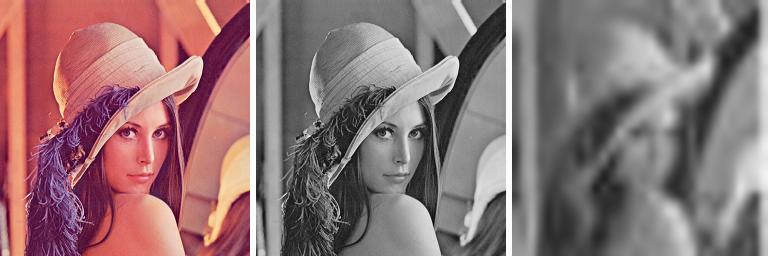
\includegraphics[scale=0.4]{Images/Lena.jpg}
		\caption{Pré-traitement d'une image}
	\end{center}
\end{figure}
Ici les dimensions d'entrées et de sorties sont comparables, nous pouvons donc "choisir" plus facilement les combinaisons de variables à effectuer pour classifier les images. Toutefois la perte d'information, due aux pré-traitements appliqués aux données, est grande, ce qui aura un impact potentiel sur la performance de notre algorithme apprenant.

Une approche un peu plus réfléchie pourrait suggérer d'une part de ne pas réduire la dimension des données non pas pendant le pré-traitement, mais surtout d'autre part, d'éviter de la réduire d'un seul coup, mais plutôt petit à petit.

\subsubsection{Pooling d'Information}
Le \emph{pooling}, signifiant \emph{mise en commun}, consiste à résumer l'information apportée par les valeurs de sorties proches en une seule valeur.
Il existe deux déclinaisons du \emph{pooling},
\begin{itemize}
	\item Le \emph{max pooling}, qui calcule le maximum des valeurs données en entrée.
	\item L'\emph{average pooling}, qui calcule la moyenne des valeurs données en entrée.
	\item Les convolutions avec une ou plusieurs \emph{strides} $> 1$
\end{itemize}
Nous allons maintenant voir un exemple de calcul d'un \emph{pooling} appliqué sur les composantes spatiales.\\
Soit $I$ un tenseur de dimensions $(C_I, H_I, W_I)$, et une fonction de \emph{pooling} définie par une fenêtre de dimension $(H_P, W_P)$, de \emph{padding} $(p_H, p_W)$ et de \emph{strides} $(s_H, s_W)$,\\
Alors $S$ sera de dimensions :
$$(C_S, H_S, W_S) = (C_I, (H_I + p_H - H_K) / s_H + 1, (W_I + p_W - W_K) / s_W + 1))$$

Ces deux déclinaisons de pooling sont utilisées dans des contextes assez différents.
\paragraph{Max-Pooling}
Le \emph{max pooling} est principalement utilisé pour réduire la dimension des données de façon spatiale, c'est une méthode robuste aux bruits ambiants, car elle ne transmet que l'information ayant le plus d'intensité.
\begin{figure}[H]
	\begin{center}
		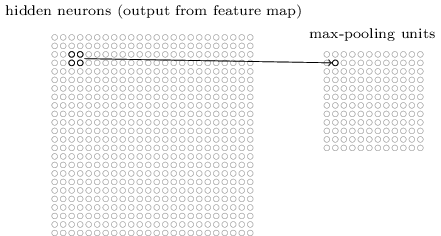
\includegraphics[scale=0.6]{Images/Pooling_Layer.png}
		\caption{\emph{Max-pooling} sur une fenêtre $(2,2)$}
	\end{center}
\end{figure}
\paragraph{Average Pooling}
L'\emph{average pooling} est principalement utilisé pour réduire la dimension des données au niveau des canaux, car elle permet de prendre en compte les valeurs des différentes \emph{features} et de les agréger.
\paragraph{Pooling par Convolution}
Les convolutions à strides $>1$ sont à l'heure actuelle \emph{à la mode}. Elles font le travail à la fois de couches de convolution, mais aussi de couches de \emph{pooling}, permettant ainsi d'une part de simplifier le modèle, ce qui réduit le nombre de \emph{floating-point operations}, mais aussi d'avoir une opération de \emph{pooling} plus "malléable", car la fonction calculée n'est pas statique, mais sera amenée à évoluer lors de la rétro-propagation.

De plus, elles sont souvent suivies de fonctions d'activation, rendant la sortie plus robuste aux bruits stochastiques.
Elle est utilisée dans plusieurs modèles très performants, justifiant ainsi sa popularité montante.
\section{Applications à la Vision par Ordinateur}
Les applications basées sur les réseaux de neurones occupent une place de plus en plus importante dans la société, le champ d'application est très large, on les retrouve notamment dans des outils de reconnaissance vocale, par exemple : Siri, Cortana; dans des outils de vision par ordinateur, utilisés par exemple dans les voitures autonomes; ou bien encore dans la création d'intelligences artificielles, liés à des jeux de réflexion, comme Deep Mind au jeu de Go, ou encore des agents conversationnels.
Pour ces applications, les performances des réseaux de neurones sont comparables voire supérieures à celles d'un humain.

Nous allons dans cette partie présenter quelques tâches liées à la vision par ordinateur, domaine dans lequel l'influence des réseaux de neurones est grande.
\subsection{Classification}
La classification est sans doute le problème le plus simple en matière de vision, il s'agit de prédire l'appartenance d'une image à une classe, généralement liée aux objets liés dans l'image.
\subsubsection{Datasets}
Un des premiers \emph{datasets} d'images pour la classification est le MNIST, composé de $70000$ images noir et blanc de $28 \times 28$ pixels, chacune contenant un chiffre manuscrit.
\begin{figure}[H]
	\begin{center}
		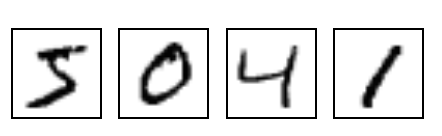
\includegraphics[scale=0.3]{Images/MNIST_Digits.png}
		\caption{Données issues de MNIST}
	\end{center}
\end{figure}
Même si l'intérêt à reconnaître les chiffres est limité, ce \emph{dataset} a longtemps servi au niveau académique de \emph{benchmark} pour comparer les différents modèles.

On citera aussi les \emph{datasets} CIFAR-10, CIFAR-100, et ImageNet.
CIFAR-10 et CIFAR-100 sont composés chacun de $60000$ images RGB de $32 \times 32$ pixels, réparties en $10$ classes pour le premier et $100$ classes pour le second.
\begin{figure}[H]
	\begin{center}
		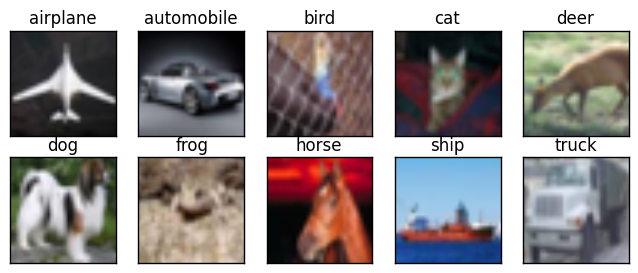
\includegraphics[scale=0.4]{Images/CIFAR-10.png}
		\caption{Données issues de CIFAR-10}
	\end{center}
\end{figure}
ImageNet contient une base de classification d'images contenant plus de $10$ millions d'URLs d'images de taille variable réparties en $1000$ classes. Les images sont majoritairement issues de sites comme Flickr.
Ce \emph{dataset}, créé en $2009$, fait l'objet d'une compétition depuis $2010$, qui a permis de réaliser des progrès impressionnants en traitement d'images.
\subsubsection{Architectures de Modèles}
En $2011$, l'erreur de classification était de $25\%$. En $2012$, le réseau de neurones convolutifs AlexNet, composé de $8$ couches, atteignait alors $16\%$ d'erreur. En $2014$, GoogLeNet ($22$ couches), suivi de près par VGG-16 ($16$ couches), remportait la compétition avec une erreur de $6.7\%$ (respectivement $7.3\%$). En $2015$, ResNet, un réseau de $152$ couches, atteignait alors $3.6\%$. En moyenne, un humain non-entraîné réalise environ $10\%$ d'erreur et un humain entraîné $5\%$.
\subsection{Détection d'Objets}
La détection d'objets consiste à prédire la classe et l'emplacement d'un ou plusieurs objets dans une image. L'emplacement d'un objet est généralement défini par une \emph{bounding box}, ou région d'intérêt, représentée par un rectangle entourant l'objet.
\begin{figure}[H]
	\begin{center}
		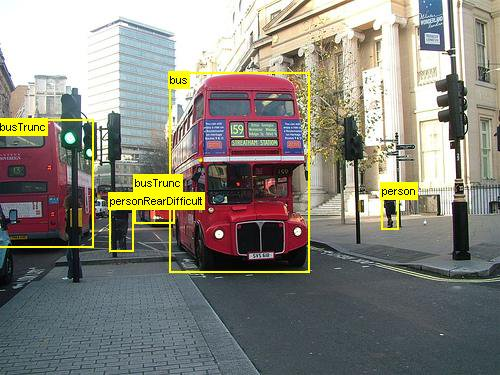
\includegraphics[scale=0.40625]{Images/Pascal_VOC_Detection.jpg}
		\caption{Image et \emph{bounding boxes} issues de Pascal VOC}
	\end{center}
\end{figure}

\subsubsection{Datasets}
Le \emph{dataset} Pascal VOC est composé de $11530$ images contenant au total $27450$ régions d'intérêt décrivant $20$ classes.

ImageNet possède aussi une base de détection d'objets contenant environ $450000$ images contenant $475000$ objets référencés répartis en $200$ classes.
\subsubsection{Architectures de Modèles}
Deux architectures remarquables sont les réseaux de type R-CNN et YOLO, l'une par ses performances exceptionnelles, l'autre par le compromis réalisé entre performances et vitesse d’exécution.

Les architectures de type R-CNN se caractérisent par un schéma de fonctionnement divisé en deux parties, la première étant un réseau de neurones assurant la localisation potentielle d'objets, la seconde étant un autre réseau de neurones dédié à la classification de chacune des zones potentielles.

Les architectures de type YOLO ont à l'inverse la particularité d'effectuer en parallèle la localisation et la classification des objets, proposant ainsi une grande vitesse d'exécution.
\subsection{Segmentation d'Images}
Comme pour la détection d'objets, la segmentation vise à identifier les objets appartenant à une classe et à les localiser sur l'image.
La différence apparaît sur la sortie produite, dans le cas de la segmentation, cela consiste à prédire, pour chaque pixel de l'image, sa classe.
La segmentation répond à des besoins de précision plus élevés que la détection d'objets, du fait de la prédiction d'un masque de la taille de l'image d'entrée.
\begin{figure}[H]
	\begin{center}
		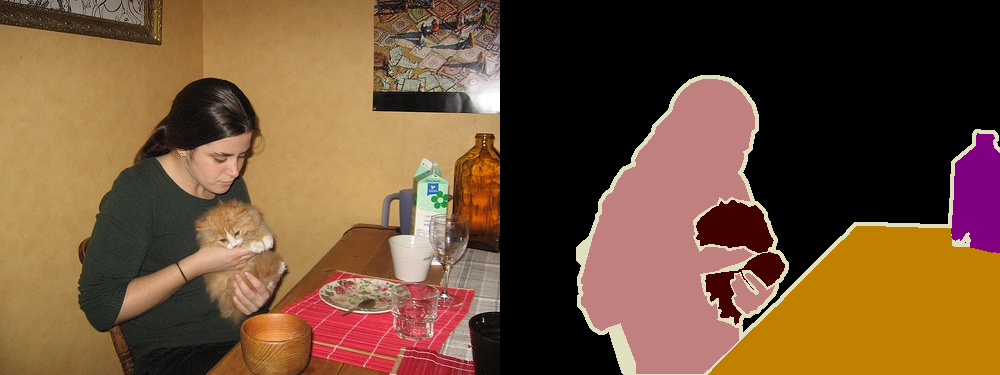
\includegraphics[scale=0.4]{Images/Pascal_VOC_Segmentation.png}
		\caption{Image et masque de classes issus de Pascal VOC}
	\end{center}
\end{figure}
Un des avantages de la segmentation d'images par rapport à la détection d'objets, outre le gain potentiel de précision, est qu'il est possible à partir d'un masque de segmentation de produire des \emph{bounding boxes} en utilisant la polygonisation des masques. L'opération inverse n'est pas vraiment intéressante puisque les polygones sont des rectangles.
\subsubsection{Datasets}
Pascal VOC possède aussi une base de segmentation d'images contenant $2913$ images décrivant $20$ classes.
Microsoft COCO (Common Objects in Context) contient $328000$ images décrivant $91$ classes.

Ces deux \emph{datasets} possèdent la particularité de segmenter les images d'une part selon la classe mais aussi en fonction de l'instance, permettant ainsi de différencier deux objets de même nature au sein d'une image.
\subsubsection{Architectures de Modèles}
Deux architectures remarquables sont les réseaux de type FCN et DeconvNet, elles utilisent toutes les deux le principe de décomposer l'image en \emph{features} par convolutions successives, puis de reconstituer l'image en image segmentée en appliquant plusieurs couches de déconvolutions.

Les architectures de type FCN reconstituent l'image en combinant les \emph{features} dé-convolutées avec les \emph{features} après \emph{pooling}.

Les architectures de type DeconvNet reconstituent l'image en utilisant des couches d'\emph{unpooling}, inversant l'effet des couches de \emph{pooling}. Nous reviendront en détail leur fonctionnement dans la suite.

\section{Conclusion}
Dans ce chapitre, nous avons tenté de donner au lecteur un aperçu du domaine de l'apprentissage machine.

Nous avons défini les réseaux de neurones, expliqué de façon détaillée le fonctionnement des réseaux de neurones, avec les notions de propagation et de rétro-propagation, ainsi que plusieurs méthodes pour améliorer la qualité de l'apprentissage.

Nous avons proposé une définition générale de la convolution, abordé le sujet de la réduction de la dimensionnalité, puis justifié l'utilité des réseaux de neurones convolutifs pour le traitement d'image, en finissant par décrire les tâches les plus courantes en vision par ordinateur.

Ce chapitre est sans doute le plus utile pour comprendre les applications évoquées dans le quatrième chapitre.
\chapter{L'Apprentissage Profond appliqué à l'Imagerie Satellite}
\section{Cartographie Automatisée par Segmentation de Classes}
La cartographie de la Terre a toujours été une des priorités de l'humain.
Les cartes ont surtout servi dans un premier temps à la navigation maritime et à une utilisation militaire. Elles ont tout le temps fait l'objet de convoitise, à tel point qu'au Portugal au XVI ème siècle le transfert de cartes à un étranger était passible de la peine de mort. L'aéronautique a ensuite permis d'affiner les cartes, mais sur des volumes toujours restreints. L'arrivée des satellites de télédétection permet alors d'acquérir quasiment en temps réel des images de la Terre.

Cette masse de données à traiter conduit à la formation de la géomatique, discipline consistant en trois activités principales la collecte, le traitement et la diffusion des données géographiques.

Il existe plusieurs types de cartographie, parmi lesquelles on retrouve :
\begin{itemize}
	\item La cartographie physique, ou topographie, répertoriant les reliefs du terrain.
	\item La cartographie humaine, mesurant des indices sociologiques.
	\item La cartographie administrative, répertoriant les frontières entre les pays.
	\item Les cartographies de type historique, biologique, etc.
\end{itemize}

Pour manipuler ces données, d'échelle parfois mondiale, on utilise des Systèmes d'Information Géographique, permettant de collecter, traiter, analyser, et enfin de présenter ces données.

Dans ce rapport, nous nous intéresserons principalement à la cartographie administrative et plus particulièrement à la cartographie d'infrastructures, telles que les routes et les bâtiments.

Aujourd'hui la majorité des données concernant les infrastructures ont été collectées "à la main".
Dans le cas d'OpenStreetMap, la base de données géographiques est remplie par les utilisateurs, soit en relevant des positions GPS en allant directement sur le terrain, soit en cartographiant depuis des images spatiales.
Ce processus est très long et ne permet pas encore une cartographie globale de toutes les infrastructures sur Terre.
Toutefois, certaines administrations publiques ont partagé des bases de données, notamment l'intégralité du cadastre français mis à disposition par la Direction générale des Finances publiques ou encore la base de données TIGER, concernant les routes, divisions administratives et points d'eau des États-Unis.
Ces initiatives ont permis de réaliser de grandes avancées dans le projet, mais ne permettent pas de cartographier toute la surface du globe.


Avec les progrès récents de l'apprentissage profond, permettant d'obtenir d'excellentes performances en vision par ordinateur, et le besoin immense d'automatiser la cartographie de la Terre, il semble intéressant d'utiliser des méthodes telle que la segmentation d'images pour identifier précisément des infrastructures.

Cela permettrait d'établir de façon automatisée des cartes détaillées de la surface du globe, permettant une utilisation civile, militaire ou encore humanitaire, permettant ainsi de comparer les cartes avant et après une catastrophe naturelle.
\subsection{Présentation des Données}
SpaceNet est une base de données d'images satellite très haute résolution pour la détection et segmentation de bâtiments.

Elle est issue de la collaboration entre CosmiQ Works, DigitalGlobe et NVIDIA.
C'est une des premières bases de données d'image très haute résolution disponible au grand public.
Les données sont hébergées par Amazon, sur les serveurs AWS S3 (Amazon Web Services Simple Storage Service).

La base de données SpaceNet actuelle fut construite en deux temps, lors des deux éditions du SpaceNet Challenge, elle couvre 5 zones géographiques :
\begin{itemize}
	\item Rio de Janeiro, Brésil.
	\item Las Vegas, États-Unis.
	\item Paris, France.
	\item Shanghai, Chine.
	\item Khartoum, Soudan.
\end{itemize}

La première édition du SpaceNet Challenge ne portait que sur Rio de Janeiro, les images provenant du satellite WorldView-2.

La seconde édition du SpaceNet Challenge portait sur Las Vegas, Paris, Shanghai et Khartoum, les images provenant du satellite WorldView-3.

\subsubsection{Images}
Les deux satellites proviennent de la famille WorldView, dont les images sont distribuées par DigitalGlobe. 

WorldView-2 fut envoyé en orbite le 8 octobre 2009, tandis que WorldView-3 fut lancé le 13 août 2014.
Les deux satellites ont des caractéristiques similaires, mais se différencient sur la résolution au sol des capteurs optiques :
\begin{center}
	\begin{tabular}{|c|c|c|}
	\hline 
	Résolution & WorldView-2 & WorldView-3 \\ 
	\hline 
	Bande Panchromatique & 0.46m & 0.31m \\ 
	\hline 
	Bandes Multispectrales & 1.84m & 1.24m \\ 
	\hline
	\end{tabular}	
\end{center}

Les satellites WorldView-2 et WorldView-3 possèdent un capteur panchromatique et $8$ capteurs multispectraux, qui décrivent les couleurs suivantes :
\begin{center}
	\begin{tabular}{|c|c|c|c|c|}
	\hline 
	Panchromatique & Côtier & Bleu & Vert & Jaune \\ 
	\hline 
	450-800nm & 400-450nm & 450-510nm & 510-580nm & 585-625nm \\ 
	\hline 
	Rouge & Rouge Frontière & Proche Infrarouge 1 & Proche Infrarouge 2 & \\ 
	\hline 
	630-690nm & 705-745nm & 775-895nm & 860-1040nm & \\ 
	\hline 
	\end{tabular}
\end{center}

Nous n'utiliserons que les données issues de la deuxième édition du SpaceNet Challenge, car les images multispectrales de la première édition n'ont pas été fusionnées avec la bande panchromatique laissant la résolution à 1.84m.

Par ailleurs, dans l'optique de rendre compatibles les modèles avec des données issues des satellites Pléiades, nous avons choisi de ne garder que 4 des 8 bandes disponibles :
\begin{itemize}
	\item Le Bleu.
	\item Le Vert.
	\item Le Rouge.
	\item Le Proche Infrarouge 1.
\end{itemize}

Les images multispectrales de la seconde édition font $650 \times 650$ pixels et ont une résolution au sol de 0.31m et sont encodées sur $16$ bits.

\begin{figure}[H]
	\begin{center}
		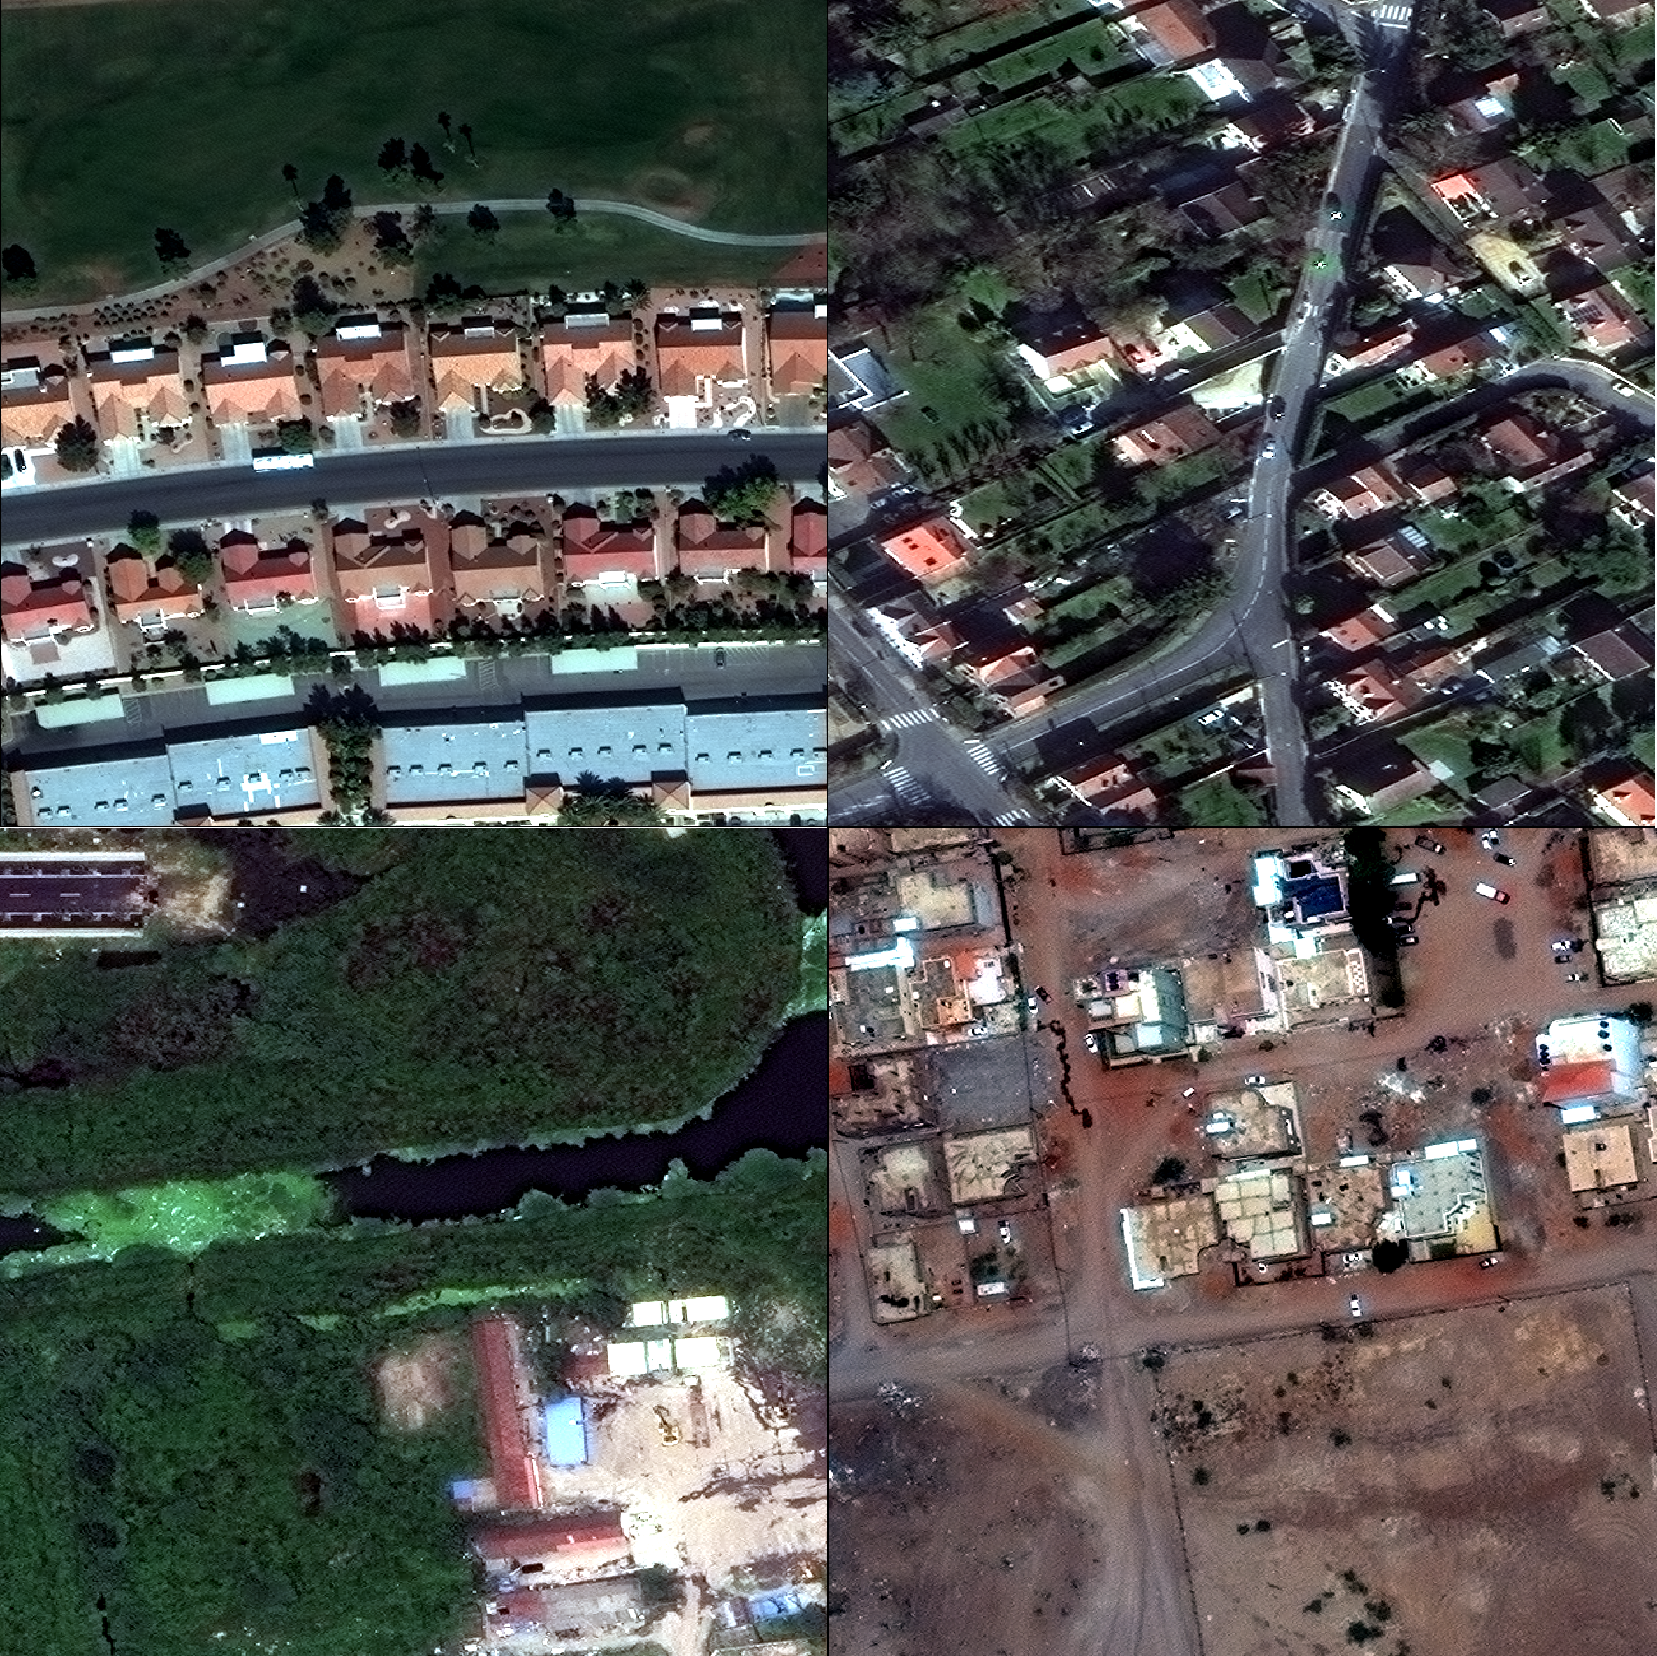
\includegraphics[scale=0.3]{Images/MUL_PAN.png}
		\caption{Images (RGB, 8-bits, Correction $[2-98]\%$) extraites des zones Vegas, Paris, Shanghai et Khartoum}
	\end{center}
\end{figure}

Voici la distribution des images en fonction des zones géographiques :
\begin{center}
	 \begin{tabular}{|c|c|c|c|c|c|}
	\hline 
	Villes & Las Vegas & Paris & Shanghai & Khartoum & Total \\ 
	\hline 
	Images & 3851 & 1148 & 4582 & 1012 & 10593 \\ 
	\hline 
	Taille & 26.1Go & 7.8Go & 31.0Go & 6.8Go & 71.7Go \\ 
	\hline 
	\end{tabular}
 \end{center} 
\subsubsection{Labels}
\paragraph{Labels issus de SpaceNet}
Le SpaceNet Challenge consiste à détecter les bâtiments visibles depuis les images satellites.

La labellisation des données a été réalisée par l'Amazon Mechanical Turk, une plateforme de crowdsourcing spécialisée dans la constitution de \emph{datasets} pour des problèmes d'intelligence artificielle.

À chaque image du \emph{dataset} correspond un fichier GeoJSON contenant l'empreinte au sol des différents bâtiments, sous forme de polygones.
Ces polygones sont représentés par des ensembles de coordonnées géodésiques, c'est-à-dire sous forme d'un couple latitude et longitude.

Voici un extrait de fichier GeoJSON issu de SpaceNet :
\begin{verbatim}
{
  "type": "FeatureCollection",
  "crs": {
    "type": "name",
    "properties": {
      "name": "urn:ogc:def:crs:OGC:1.3:CRS84"
    }
  },
  "features": [
    {
      "type": "Feature",
      "properties": {
        "OBJECTID": 0,
        "FID_VEGAS_": 0,
        "Id": 0,
        "FID_Vegas": 0,
        "Name": "None",
        "AREA": 0.000000,
        "Shape_Leng": 0.000000,
        "Shape_Le_1": 0.000000,
        "SISL": 0.000000,
        "OBJECTID_1": 0,
        "Shape_Le_2": 0.000000,
        "Shape_Le_3": 0.000811,
        "Shape_Area": 0.000000,
        "partialBuilding": 1.000000,
        "partialDec": 0.556769
      },
      "geometry": {
        "type": "Polygon",
        "coordinates": [
          [
            [-115.302252599989529, 36.208218543364502, 0.0],
            [-115.302260806999982, 36.208218603000034, 0.0], 
            [-115.302261041999941, 36.208197527000038, 0.0]
            [...]
          ]
        ]
      }
    }
[...]
}
\end{verbatim}
Le \emph{dataset} SpaceNet ne contient que des polygones.
Il existe, pour le format GeoJSON, plusieurs types d'objets géométriques simples:
\begin{itemize}
	\item \emph{Point}, représentant un point.
	\item \emph{LineString}, un ensemble ouvert ou fermé de points.
	\item \emph{Polygon}, une surface délimitée par un ensemble fermé de points. Par exemple, un triangle ABC sera représenté par ABCA.
\end{itemize}
\paragraph{Labels issus d'OpenStreetMap}
Les labels de SpaceNet, produit par l'Amazon Mechanical Turk, ne localisent que les bâtiments dans les images. Cependant d'autres informations directement observables depuis les images existent, comme par exemple les routes, ou encore les cours d'eau.
C'est pourquoi il a été jugé intéressant de compléter les labels originels de SpaceNet par des labels issus d'OpenStreetMap.
Ces labels sont disponibles au format GeoJSON et il est facile de les récupérer depuis l'API d'OpenStreetMap.
Cependant ces labels ne sont pas de même qualité que ceux provenant du \emph{dataset} SpaceNet, il est important de garder à l'esprit que ces labels sont issus d'un projet communautaire, ils peuvent donc faire l'objet d'imprécisions, par exemple concernant la localisation des éléments géographiques, potentiellement due aux imprécisions de GPS amateurs, ou parfois tout simplement manquants, car personne n'a encore répertorié la zone géographique en question.
\paragraph{Rasterisation des Labels}
Les labels issus de SpaceNet ou d'OpenStreetMap sont proposés sous forme vectorielle et donc par conséquent utilisables pour de la détection d'objets.
Les labels vectoriels, au même titre que les images vectorielles, possèdent l'avantage d'être quasiment invariants à la résolution de l'image.
Mais pour réaliser de la segmentation d'images, il nous faut pouvoir produire un label au format matriciel de même dimensions que l'image d'entrée.
L'opération permettant de produire une image matricielle à partir d'une image vectorielle s'appelle rasterisation. Bien que l'opération ne soit pas bijective, car irréversible à cause de la résolution finie de l'image matricielle. Il existe une opération effectuant la transformation inverse, on parlera alors de polygonisation.
L'opération de rasterisation consiste à produire, à partir des données vectorielles, ainsi que des dimensions et la résolution de l'image souhaitée, une image matricielle où chaque pixel prend une valeur selon si il est contenu ou non dans un polygone.
\begin{figure}[H]
	\begin{center}
		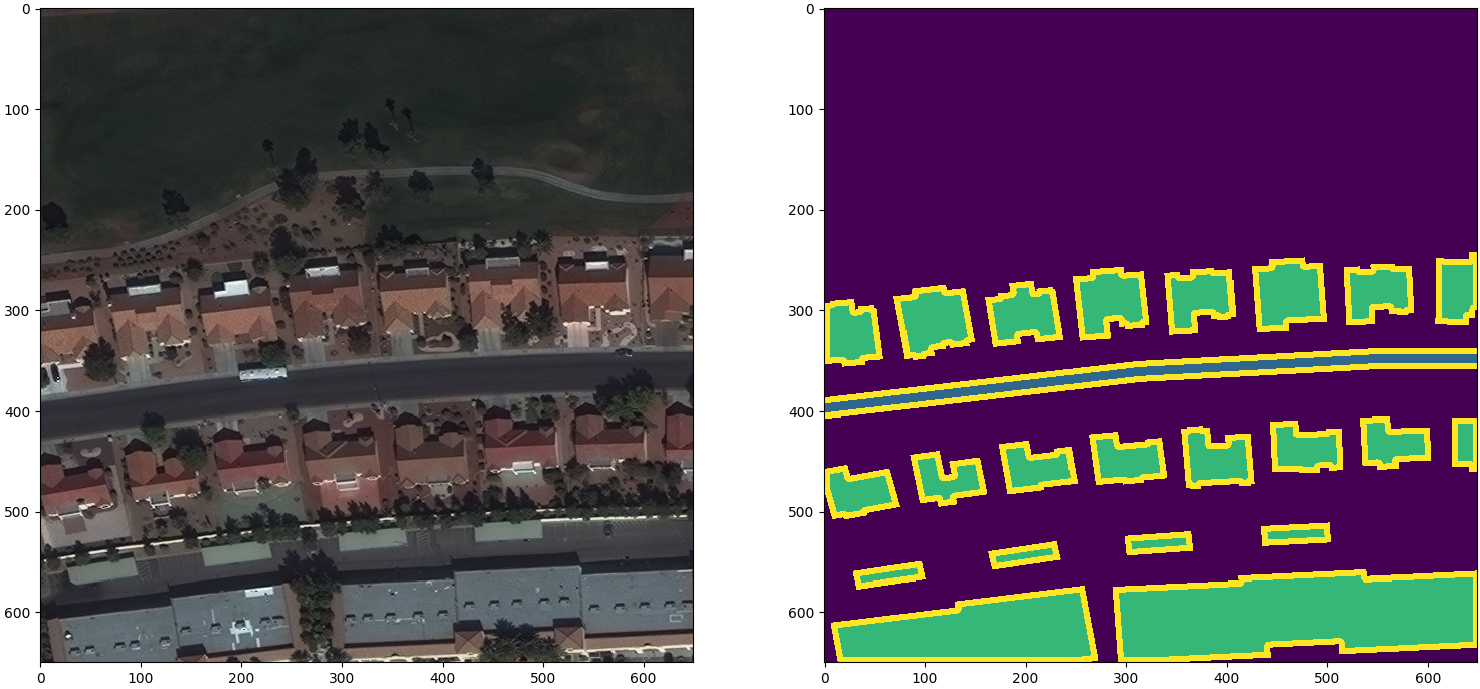
\includegraphics[scale=0.3]{Images/MUL_PAN_Label_Vegas.png}
		\caption{Image et Masque de Segmentation produit par couplage des labels issus de SpaceNet et d'OpenStreetMap (Las Vegas)}
	\end{center}
\end{figure}
Les labels d'OpenStreetMap sont très libres au niveau des informations qu'ils contiennent, le champ \emph{properties}, donnant des informations sur l'objet décrit, n'est pas systématiquement présent ou partiellement renseigné. Il est donc difficile de catégoriser chaque donnée.

Nous avons choisi dans le cas où les labels de SpaceNet sont combinés avec ceux provenant d'OpenStreetMap, que seuls les \emph{Polygons} et les \emph{LineStrings} non fermées seront rasterisés.

Cela dégrade quelque peu la qualité des données car nous considérons que tous les \emph{Polygons} représentent des bâtiments et que toutes les \emph{LineStrings} représentent des routes. Même si les \emph{Polygons} représentent quasiment tout le temps des bâtiments, les \emph{LineStrings} représentent parfois des cours d'eau, ou encore des délimitations administratives.

De plus, les \emph{LineStrings} forment des courbes, elles ont donc une aire nulle, or les routes sont des surfaces, il a donc fallu choisir arbitrairement la largeur d'une route à rasteriser. Nous avons choisi $3$ mètres afin d'être sûr de ne pas empiéter sur des bâtiments alentours.

C'est pourquoi il faudra prendre en compte ces erreurs contenues dans le \emph{dataset} au moment d'analyser les résultats des différents modèles.

Le contour des objets rasterisés, ici en jaune, n'appartient pas à la même classe que son objet, ceci est fait pour pallier aux erreurs de localisation des objets. En effet un pixel faisant parti du contour d'un objet ne sera pas évalué lors du calcul de la perte et de la précision, cela permet aux modèles de ne pas se focaliser sur les détails mais plus sur le cœur de l'objet.
\subsection{Calcul GPU et Caffe}
\subsubsection{Calcul GPU}
Dans le chapitre portant sur l'apprentissage profond, nous avons proposé les algorithmes de propagation et de rétro-propagation en version matricielle.

Les réseaux de neurones de type \emph{feedforward} sont entièrement parallélisables.

L'intérêt du calcul matriciel est de pouvoir le distribuer sur plusieurs processeurs.

Les processeurs CPU sont très rapides, mais ne sont pas optimisés pour des calculs entièrement parallélisables, car le nombre de cœurs dans un processeur CPU est très limité pour diverses raisons.

Les processeurs GPU, quant à eux sont moins rapides, mais possèdent beaucoup plus de cœurs que les processeurs GPU, le rapport est de l'ordre de $10^2$. Néanmoins une contrainte subsiste : la mémoire GPU.

La mémoire GPU coûte beaucoup plus cher, de manière générale, que la mémoire CPU. Néanmoins si l'ensemble du réseau de neurones rentre en mémoire GPU, alors un processeur GPU est généralement 50 à 100 plus performant qu'un processeur CPU.

C'est pour toutes ces raisons que nous allons employer des \emph{frameworks} implémentant le calcul GPU.

Nous utiliserons l'API de calcul GPU \emph{CUDA}, développé par NVIDIA.

\subsubsection{Caffe}
Le \emph{framework} utilisé dans les applications que nous avons développées s'appelle Caffe.

Il développé sous license BSD par le \emph{Berkeley AI Research} et une communauté de contributeurs.

Il est très utilisé en milieu académique pour plusieurs raisons :
\begin{itemize}
	\item Il est très facile et encouragé de développer son propre \emph{fork} de Caffe.
	\item La syntaxe, en \emph{protobuf}, permettant de créer des modèles est très éloignée de l'implémentation machine.
	\item Les modèles produits sont facilement réutilisables, facilitant leur diffusion.
\end{itemize}
\subsection{Expériences}
Nous souhaitons présenter deux expériences ayant produit les résultats les plus significatifs.

La première expérience couvre les quatre zones géographiques, c'est-à-dire Las Vegas, Paris, Shanghai et Khartoum, et utilise uniquement les labels provenant de SpaceNet.
La segmentation réalisée est binaire, car cela revient à prédire pour chaque pixel de l'image son appartenance à un bâtiment ou non.

La seconde expérience exploite uniquement les données de la région de Las Vegas,  et utilise des labels provenant de SpaceNet et d'OpenStreetMap.
La segmentation sera multi-classes, il faudra en effet prédire pour chaque pixel de l'image son appartenance à un bâtiment, ou une route, ou bien d'aucune de ces deux classes.

Avant de présenter chacune des expériences et de comparer les modèles utilisés, nous allons d'abord présenter l'architecture ayant inspiré ces modèles, nommée DeconvNet.

\subsubsection{DeconvNet}

DeconvNet est un réseau de neurones créé par H.Noh, en 2015, de l'université POSTECH, Corée du Sud.

Nous allons d'abord décrire son architecture, puis discuter des avantages et inconvénients de celle-ci.

DeconvNet est un réseau convolutif introduisant un nouveau type de couche, l'\emph{unpooling}, faisant la particularité de ce modèle.

DeconvNet est un réseau de neurones composé de deux parties, la première est composée de couches de convolution et de \emph{pooling}, décomposant l'image en une \emph{map de features}; et la seconde est composée de couches de déconvolution et d'\emph{unpooling}, construisant à partir de la \emph{map de features} l'image segmentée.

La première partie n'est autre que le réseau de neurones VGG-16, classé second lors de l'ILSVRC 2014.
La seconde partie peut être vu comme le symétrique de la première reconstruisant l'image segmentée.

\paragraph{Unpooling}
Le principe d'une couche de \emph{max pooling} est de filtrer le bruit tout en réduisant la dimension des données. Cette réduction de la dimension est souvent de nature spatiale, créant une perte d'informations spatiales.
Pour pallier à cela, H.Noh a créé le concept de couche d'\emph{unpooling}, produisant l'effet quasi-inverse.
L'idée est la suivante, si lors de l'opération de \emph{pooling}, nous retenons les indices des activations maximales, alors nous pouvons ensuite reconstruire une \emph{carte à trous} des activations dans la dimension originelle.
Voici un schéma décrivant l'opération d'\emph{unpooling} :
\begin{figure}[H]
	\begin{center}
		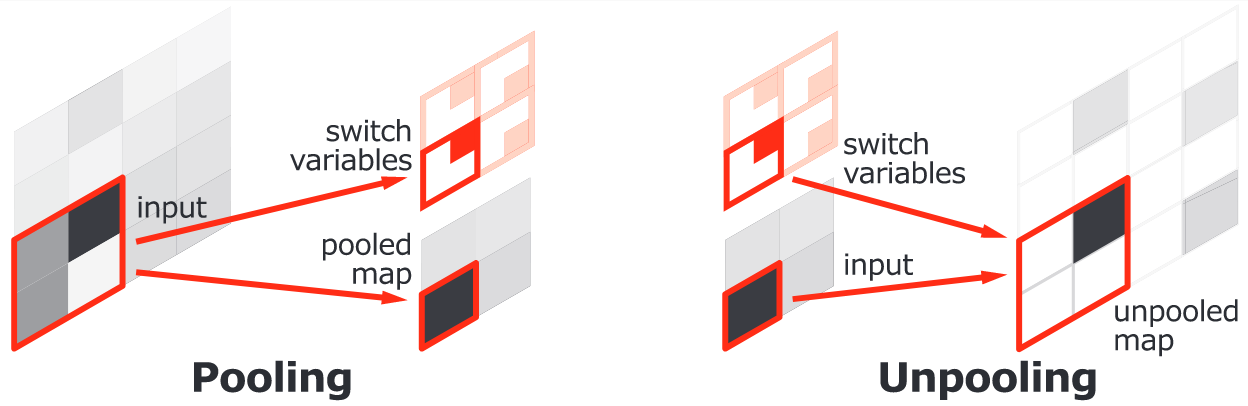
\includegraphics[scale=0.3]{Images/Unpooling.png}
		\caption{Couches de \emph{pooling} et d'\emph{unpooling}}
	\end{center}
\end{figure}
Comme on peut le voir dans la couche de \emph{pooling}, l'activation la plus élévée, ici la plus sombre, est transmise dans la \emph{map de features}, ainsi que sa position dans la \emph{map des indices}. Alors lors de l'\emph{unpooling}, nous réutiliserons la \emph{map des indices} pour recréer la \emph{map de features} à ses dimensions précédentes.

\paragraph{Déconvolution}
Une couche de convolution a effectue un produit matriciel entre un noyau et une fenêtre d'une \emph{map de  features}, qui grossièrement dit, revient calculer une moyenne pondérée sur un ensemble de valeurs spatialement proches.
Elle permet ainsi de calculer de nouvelles \emph{features} à partir d'une \emph{map de features} existante.
La déconvolution effectue l'opération inverse, c'est-à-dire de partir d'une \emph{feature} pour produire une \emph{map de features}
Voici un schéma décrivant la relation entre une convolution et une déconvolution :
\begin{figure}[H]
	\begin{center}
		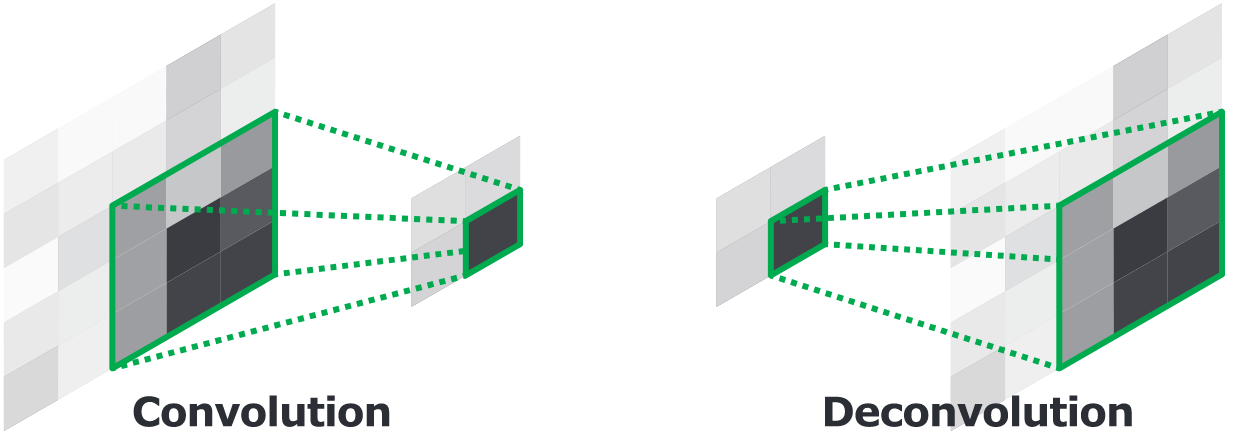
\includegraphics[scale=0.3]{Images/Deconvolution.png}
		\caption{Couches de convolution et de déconvolution}
	\end{center}
\end{figure}
Comme on peut le voir, la couche de convolution agrège des entrées voisines par une moyenne pondérée qui sera transmise à la couche suivante.
La couche de déconvolution réalise l'opération inverse, à partir d'une seule entrée elle reconstitue le voisinage d'entrées.

\paragraph{Architecture}
Après avoir expliqué le fonctionnement des couches de déconvolution et d'\emph{unpooling}, nous allons présenter l'architecture de DeconvNet et expliquer certaines particularités.

Voici le détail de l'architecture de DeconvNet, en ommettant les couches de \emph{Batch Normalization} et d'activation ReLU présentes après chaque couche de convolution:
\begin{center}
	\begin{tabular}{|c|c|c|c|c|c|}
	\hline 
	Couche & Noyau & Features & Stride & Pad & Dimensions en sortie \\ 
	\hline 
	Input & - & - & - & - & $(4, 224, 224)$\\ 
	\hline 
	conv1\_$1$ & $(3, 3)$ & 64 & 1 & 1 & $(64, 224, 224)$ \\
	\hline 
	conv1\_$2$ & $(3, 3)$ & 64 & 1 & 1 & $(64, 224, 224)$ \\
	\hline 
	pool1 & $(2, 2)$ & - & 2 & 0 & $(64, 112, 112)$ \\
	\hline 
	conv2\_$1$ & $(3, 3)$ & 128 & 1 & 1 & $(128, 112, 112)$ \\
	\hline 
	conv2\_$2$ & $(3, 3)$ & 128 & 1 & 1 & $(128, 112, 112)$ \\
	\hline 
	pool2 & $(2, 2)$ & - & 2 & 0 & $(128, 56, 56)$ \\
	\hline 
	conv3\_$1$ & $(3, 3)$ & 256 & 1 & 1 & $(256, 56, 56)$ \\
	\hline 
	conv3\_$2$ & $(3, 3)$ & 256 & 1 & 1 & $(256, 56, 56)$ \\
	\hline 
	conv3\_$3$ & $(3, 3)$ & 256 & 1 & 1 & $(256, 56, 56)$ \\
	\hline 
	pool3 & $(2, 2)$ & - & 2 & 0 & $(256, 28, 28)$ \\
	\hline 
	conv4\_$1$ & $(3, 3)$ & 512 & 1 & 1 & $(512, 28, 28)$ \\
	\hline 
	conv4\_$2$ & $(3, 3)$ & 512 & 1 & 1 & $(512, 28, 28)$ \\
	\hline 
	conv4\_$3$ & $(3, 3)$ & 512 & 1 & 1 & $(512, 28, 28)$ \\
	\hline 
	pool4 & $(2, 2)$ & - & 2 & 0 & $(512, 14, 14)$ \\
	\hline 
	conv5\_$1$ & $(3, 3)$ & 512 & 1 & 1 & $(512, 14, 14)$ \\
	\hline
	conv5\_$2$ & $(3, 3)$ & 512 & 1 & 1 & $(512, 14, 14)$ \\
	\hline
	conv5\_$3$ & $(3, 3)$ & 512 & 1 & 1 & $(512, 14, 14)$ \\
	\hline
	pool5 & $(2, 2)$ & - & 2 & 0 & $(512, 7, 7)$ \\
	\hline
	fc6 & $(7, 7)$ & 4096 & 1 & 0 & $(4096, 1, 1)$ \\
	\hline
	fc7 & $(1, 1)$ & 4096 & 1 & 0 & $(4096, 1, 1)$ \\
	\hline
	deconv-fc6 & $(7, 7)$ & 512 & 1 & 0 & $(512, 7, 7)$ \\
	\hline
	unpool5 & $(2, 2)$ & - & 2 & 0 & $(512, 14, 14)$ \\
	\hline
	deconv5\_$1$ & $(3, 3)$ & 512 & 1 & 1 & $(512, 14, 14)$ \\
	\hline
	deconv5\_$2$ & $(3, 3)$ & 512 & 1 & 1 & $(512, 14, 14)$ \\
	\hline
	deconv5\_$3$ & $(3, 3)$ & 512 & 1 & 1 & $(512, 14, 14)$ \\
	\hline
	unpool4 & $(2, 2)$ & - & 2 & 0 & $(512, 28, 28)$ \\
	\hline
	deconv4\_$1$ & $(3, 3)$ & 512 & 1 & 1 & $(512, 28, 28)$ \\
	\hline
	deconv4\_$2$ & $(3, 3)$ & 512 & 1 & 1 & $(512, 28, 28)$ \\
	\hline
	deconv4\_$3$ & $(3, 3)$ & 256 & 1 & 1 & $(256, 28, 28)$ \\
	\hline
%	\end{tabular} 
%\end{center}
%\begin{center}
%	\begin{tabular}{|c|c|c|c|c|c|}
%	\hline 
%	Couche & Noyau & Features & Stride & Pad & Dimensions en sortie \\ 
%	\hline
	unpool3 & $(2, 2)$ & - & 2 & 0 & $(256, 56, 56)$ \\
	\hline
	deconv3\_$1$ & $(3, 3)$ & 256 & 1 & 1 & $(256, 56, 56)$ \\
	\hline
	deconv3\_$2$ & $(3, 3)$ & 256 & 1 & 1 & $(256, 56, 56)$ \\
	\hline
	deconv3\_$3$ & $(3, 3)$ & 128 & 1 & 1 & $(128, 56, 56)$ \\
	\hline
	unpool2 & $(2, 2)$ & - & 2 & 0 & $(128, 112, 112)$ \\
	\hline
	deconv2\_$1$ & $(3, 3)$ & 128 & 1 & 1 & $(128, 112, 112)$ \\
	\hline
	deconv2\_$2$ & $(3, 3)$ & 64 & 1 & 1 & $(64, 112, 112)$ \\
	\hline
	unpool1 & $(2, 2)$ & - & 2 & 0 & $(64, 224, 224)$ \\
	\hline
	deconv1\_$1$ & $(3, 3)$ & 64 & 1 & 1 & $(64, 224, 224)$ \\
	\hline
	deconv1\_$2$ & $(3, 3)$ & 64 & 1 & 1 & $(64, 224, 224)$ \\
	\hline
	Output & $(1, 1)$ & $X$ & 1 & 0 & $(X, 224, 224)$ \\
	\hline
	\end{tabular} 
\end{center}
On peut tout de suite remarquer que le réseau est symétrique, la couche \emph{fc7} étant le point central de cette symétrie.

Comme évoqué précédemment, l'idée est dans un premier temps de décomposer l'image en \emph{map de features} par convolutions successives (et de \emph{pooling}), puis dans un second temps de reconstituer une version segmentée de l'image par déconvolution (et d'\emph{unpooling}).

La première partie du réseau, de \emph{conv1\_$1$} à \emph{fc7}, n'est autre que le réseau VGG-16, crée par K.Simonyan, classé second lors de l'ILSVRC 2014.

Ce réseau est l'un des plus utilisés (ou réutilisés, comme ici) en vision par ordinateur, car il est d'une extrême simplicité.
Il n'utilise que des convolutions de noyau $(3, 3)$, qui sont jugées robustes pour l'apprentissage.

On peut remarquer que les convolutions sont regroupées ici en 5 blocs, chaque bloc étant séparé par une couche de \emph{pooling}.
Si l'on fait abstraction des couches d'activation ReLU, chaque bloc de convolution se résume comme une composée de convolutions.
Or on peut remarquer que deux convolutions $(3, 3)$ successives équivalent à une convolution $(5, 5)$, venant de la propriété de majoration du support :

Soit $f$ et $g \in L^2(\mathbb{R}^n)$ alors,
$$supp(f * g) \subset \overline{supp(f) + supp(g)} = \{ x + y | x \in supp(f), y \in supp(g) \}$$

Ainsi l'architecture VGG-16 peut être alors approximée simplement par un réseau comprenant $5$ couches de convolutions entrecoupés de couches d'activation et de \emph{pooling}, les deux premières étant $(5,5)$ et les trois suivantes étant $(7,7)$.
Ce modèle serait bien moins stable à l'apprentissage, mais aussi moins performant, car l'insertion d'activations entre les convolutions permet d'encore mieux séparer les plans de solutions.

La seconde partie du réseau, propre à DeconvNet, utilise les couches de déconvolution et d'\emph{unpooling} détaillées précédemment. On remarquera aussi l'utilisation de déconvolutions successives de noyau $(3, 3)$, pour les mêmes raisons que les convolutions de la première partie.

Enfin la couche de sortie effectue le mapping entre les \emph{features} produite et le nombre de classes souhaitées en sortie, par une convolution de noyau $(1, 1)$.

La philosophie de l'architecture DeconvNet pourrait se résumer à dans un premier temps décomposer l'image en \emph{features} très profondes à travers 13 couches de convolution entrecoupées de \emph{pooling}, puis de réduire l'image en un vecteur de 4096 \emph{features}, avant de reconstituer une image segmentée à travers 13 couches de déconvolution entrecoupées d'\emph{unpooling}.

\paragraph{Avantages et Inconvénients}
Nous allons à présent lister les différents avantages et inconvénients de l'architecture DeconvNet.
Les avantages sont les suivants :
\begin{itemize}
	\item Simplicité et élégance de conception.
	\item Réutilisation de VGG-16, modèle très performant en vision par ordinateur.
	\item Grande finesse de segmentation des détails des objets.
	\item $69\%$ de précision sur PASCAL VOC 2012, offrant les meilleures performances en 2015.
\end{itemize}
Les inconvénients sont les suivants :
\begin{itemize}
	\item Très grand nombre de \emph{FLOPs}, nécessitant des GPUs très puissantes.
	\item Apprentissage complexe, divisé en deux phases, chacune ayant un ensemble d'apprentissage distinct.
\end{itemize}

\subsubsection{Première Expérience}
N'ayant pas de cartes graphiques suffisamment puissantes en terme de capacité de mémoire, seulement $4$ Go, il n'a pas été possible de reprendre l'architecture de DeconvNet et l'entraîner à la segmentation d'images avec les labels provenant uniquement de SpaceNet, ce qui en fait de la segmentation binaire.

Des architectures, réutilisant les notions de convolution, \emph{pooling}, déconvolution et \emph{unpooling}, ont été esquissées.
Ces architectures peuvent être vues comme des versions allégées de DeconvNet.

\paragraph{Architectures}
Afin de produire et entraîner une version allégée de DeconvNet, nous avons décidé, pour la première expérience, d'enlever des couches proche du \emph{centre de symétrie} du réseau.

En effet, les couches les plus gourmandes en matières de nombre de paramètres d'apprentissage sont les couches \emph{fc6} et \emph{deconv-fc6}, car ce sont des convolutions ayant des noyaux de dimensions $(4096, 512, 7, 7)$ et $(512, 4096, 7, 7)$, soit $102760448 \approx 1.02 \times 10^8$ paramètres à ajuster pour chacune de ces deux couches, ce qui représente environ $822$ Mo par couche.

Nous avons donc défini plusieurs modèles allégés de DeconvNet dans l'optique de les comparer, la logique de leur conception est simple, on pouvait remarquer que DeconvNet était constitué de 11 blocs de couches, répartis en 5 blocs de convolution, 5 bloc de déconvolution et 1 bloc central.
Nous avons donc décider de créer des modèles contenant 5 et 7 blocs, en voici leur définitions :
\begin{center}
	\begin{tabular}{|c|c|c|c|c|c|c|c|}
	\hline 
	Couche & Noyau & Features & Stride & Pad & Dimensions en sortie & Deconv5 & Deconv7\\ 
	\hline 
	Input & - & - & - & - & $(4, 224, 224)$ & \checkmark & \checkmark \\ 
	\hline 
	conv1\_$1$ & $(3, 3)$ & 64 & 1 & 1 & $(64, 224, 224)$ & \checkmark & \checkmark \\
	\hline 
	conv1\_$2$ & $(3, 3)$ & 64 & 1 & 1 & $(64, 224, 224)$ & \checkmark & \checkmark \\
	\hline 
	pool1 & $(2, 2)$ & - & 2 & 0 & $(64, 112, 112)$ & \checkmark & \checkmark \\
	\hline 
	conv2\_$1$ & $(3, 3)$ & 128 & 1 & 1 & $(128, 112, 112)$ & \checkmark & \checkmark \\
	\hline 
	conv2\_$2$ & $(3, 3)$ & 128 & 1 & 1 & $(128, 112, 112)$ & \checkmark & \checkmark \\
	\hline 
	pool2 & $(2, 2)$ & - & 2 & 0 & $(128, 56, 56)$ & \checkmark & \checkmark \\
	\hline 
	conv3\_$1$ & $(3, 3)$ & 256 & 1 & 1 & $(256, 56, 56)$ & \checkmark & \checkmark \\
	\hline 
	conv3\_$2$ & $(3, 3)$ & 256 & 1 & 1 & $(256, 56, 56)$ & \checkmark & \checkmark \\
	\hline 
	conv3\_$3$ & $(3, 3)$ & 256 & 1 & 1 & $(256, 56, 56)$ & - & \checkmark \\
	\hline 
	pool3 & $(2, 2)$ & - & 2 & 0 & $(256, 28, 28)$ & - & \checkmark \\
	\hline 
	conv4\_$1$ & $(3, 3)$ & 512 & 1 & 1 & $(512, 28, 28)$ & - & \checkmark \\
	\hline 
	conv4\_$2$ & $(3, 3)$ & 512 & 1 & 1 & $(512, 28, 28)$ & - & \checkmark \\
	\hline
	deconv4\_$3$ & $(3, 3)$ & 256 & 1 & 1 & $(256, 28, 28)$ & - & \checkmark \\
	\hline
	unpool3 & $(2, 2)$ & - & 2 & 0 & $(256, 56, 56)$ & - & \checkmark \\
	\hline
	deconv3\_$1$ & $(3, 3)$ & 256 & 1 & 1 & $(256, 56, 56)$ & - & \checkmark \\
	\hline
	deconv3\_$2$ & $(3, 3)$ & 256 & 1 & 1 & $(256, 56, 56)$ & - & \checkmark \\
	\hline
	deconv3\_$3$ & $(3, 3)$ & 128 & 1 & 1 & $(128, 56, 56)$ & \checkmark & \checkmark \\
	\hline
	unpool2 & $(2, 2)$ & - & 2 & 0 & $(128, 112, 112)$ & \checkmark & \checkmark \\
	\hline
	deconv2\_$1$ & $(3, 3)$ & 128 & 1 & 1 & $(128, 112, 112)$ & \checkmark & \checkmark \\
	\hline
	deconv2\_$2$ & $(3, 3)$ & 64 & 1 & 1 & $(64, 112, 112)$ & \checkmark & \checkmark \\
	\hline
	unpool1 & $(2, 2)$ & - & 2 & 0 & $(64, 224, 224)$ & \checkmark & \checkmark \\
	\hline
	deconv1\_$1$ & $(3, 3)$ & 64 & 1 & 1 & $(64, 224, 224)$ & \checkmark & \checkmark \\
	\hline
	deconv1\_$2$ & $(3, 3)$ & 64 & 1 & 1 & $(64, 224, 224)$ & \checkmark & \checkmark \\
	\hline
	Output & $(1, 1)$ & 2 & 1 & 0 & $(2, 224, 224)$ & \checkmark & \checkmark \\
	\hline
	\end{tabular} 
\end{center}

Comme nous pouvons le voir, les deux modèles possèdent un bloc central différent de DeconvNet.
Dans DeconvNet, l'entrée était de dimension $(512, 7, 7)$, puis ramené à un vecteur de 4096 \emph{features} dans la couche $fc6$, ce qui dé-spatialisait entièrement l'information.
Ici dans le bloc central l'information reste spatialisée, car on ne passe pas de $(256, 56, 56)$ (ou $(512, 28, 28)$) à un vecteur de $n$ \emph{features}.

\paragraph{Hyper-paramètres}
Nous allons à présent lister les hyper-paramètres liés aux apprentissages effectués.
\subparagraph{Algorithme de Descente de Gradient}
Nous avons choisi d'utiliser, comme algorithme de descente la variante \emph{Adam}, signifiant \emph{Adaptative Moment Estimation}, qui utilise le moment des gradients précédents et qui moyenne l'amplitude des gradients calculés.
Nous avons utilisé les paramètres préconisés par les auteurs, à savoir $\beta = 0.9$, $\gamma = 0.999$ et $\alpha = 0.1$.
Pour plus de détails, voir en annexe.
\subparagraph{Régularisation $L^2$}
Nous avons choisi d'utiliser, comme taux de régularisation $L^2$, $\lambda = 0.0005$, qui est une valeur couramment choisie en vision par ordinateur.
\subparagraph{Proportions de données d'apprentissage}
Il est courant dans le cas de la segmentation d'images de prendre $90\%$ des données pour l'ensemble d'apprentissage et $10\%$ pour l'ensemble de validation.
\subparagraph{Taille d'un \emph{mini-batch}}
Nous avons fixé la taille d'un mini-batch à $64$, valeur communément utilisée dans la littérature.
\subparagraph{Nombre d'itérations}
Nous avons fixé à $50000$ le nombre d'itérations lors de l'apprentissage, valeur jugée suffisante, au delà de laquelle si un modèle n'a toujours pas suffisamment appris, alors sa capacité sera remise en question.
\paragraph{Résultats}
\subparagraph{Graphes des Pertes}
Voici le graphe des pertes du modèle Deconv5 :
\begin{figure}[H]
	\begin{center}
		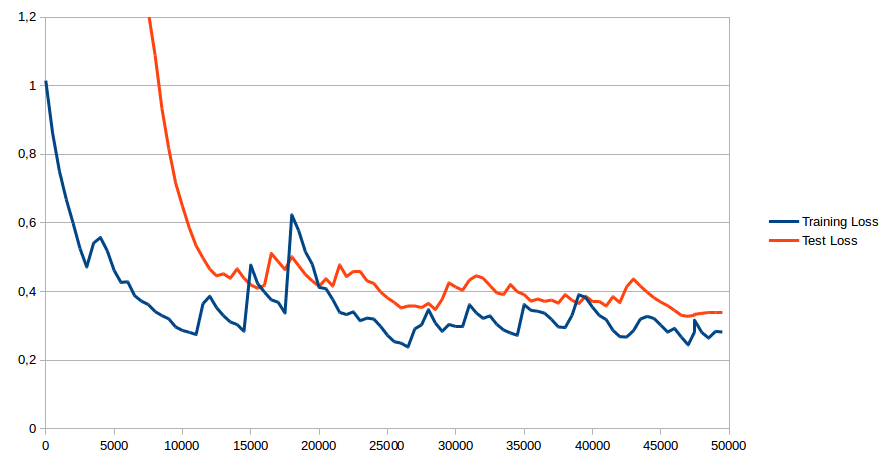
\includegraphics[scale=0.6]{Images/Losses_Deconv5.png}
		\caption{Graphe de la fonction de perte pour le modèle Deconv5}
	\end{center}
\end{figure}
L'écart entre l'erreur d'apprentissage et l'erreur de test est faible, on peut donc conclure qu'il n'y a peu ou pas de sur-apprentissage.
De plus l'erreur ne varie pas de façon particulièrement erratique, ce qui est signe d'un bon apprentissage.

Voici le graphe des pertes du modèle Deconv7 :
\begin{figure}[H]
	\begin{center}
		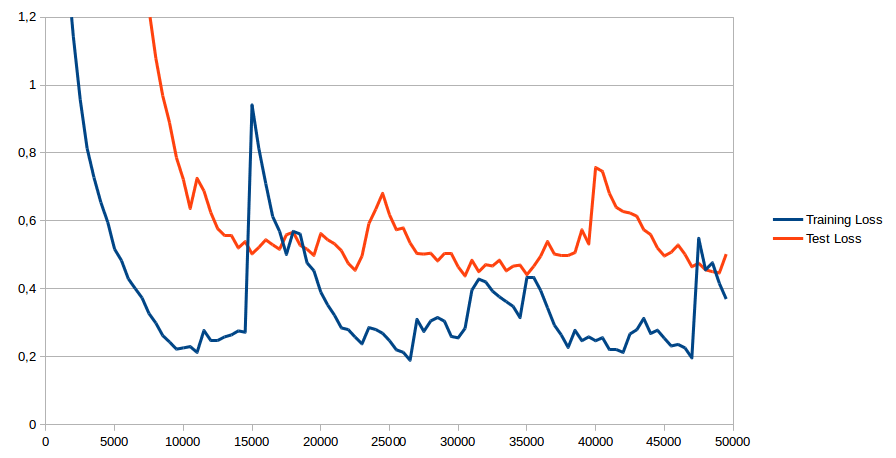
\includegraphics[scale=0.6]{Images/Losses_Deconv7.png}
		\caption{Graphe de la fonction de perte pour le modèle Deconv7}
	\end{center}
\end{figure}
Ici l'écart entre l'erreur d'apprentissage et l'erreur de test est grande, ce qui laisse supposer du sur-apprentissage.
De plus l'erreur varie de façon erratique, signe d'un mauvais apprentissage.
\subparagraph{Analyse des Résultats}
Voyons à présent les meilleures performances des modèles.

La précision est calculée de la façon suivante :
$$Accuracy(X) = \frac{1}{|X|}\sum_{x \in X} {\frac{1}{|I| \times |J|}\sum_{i \in I, j \in J} {\mathds{1}_{\{x_{i, j} = l_{i, j}\}}}}$$
Avec $x_{i, j}$, l'\emph{argmax} de couche \emph{output} du modèle aux coordonnées $(i, j)$, et $l_{i,j}$, la valeur du label aux coordonnées $(i, j)$.

Ce qui revient à calculer la moyenne sur toutes les données de l'ensemble, de la moyenne du nombre de pixels correctement classifiés sur le nombre total de pixels.

Pour Deconv5, l'itération 46500 semble être la meilleure.

La précision globale est de $0.892154$, ce qui signifie qu'environ $\frac{9}{10}$ des pixels sont correctement classifiés.

La matrice de confusion est la suivante :
\begin{center}
	\begin{tabularx}{0.5\textwidth}{c|c c|}
		Réel/Prédit & Bâtiment & Absence \\
		\hhline{---}
		Bâtiment & 0.747 \cellcolor[gray]{.8} & 0.253 \\
		Absence & 0.114 & 0.886 \cellcolor[gray]{.8}\\
		\hhline{~--}
	\end{tabularx}
\end{center}


Pour Deconv7, l'itération 47000 semble être la meilleure.

La précision globale est de $0.911284$.

La matrice de confusion est la suivante :
\begin{center}
	\begin{tabularx}{0.5\textwidth}{c|c c|}
		Réel/Prédit & Bâtiment & Absence \\
		\hhline{---}
		Bâtiment & 0.672245 \cellcolor[gray]{.8} & 0.327755 \\
		Absence & 0.080381 & 0.919619 \cellcolor[gray]{.8}\\
		\hhline{~--}
	\end{tabularx}
\end{center}

On remarque ici que le modèle a tendance à mieux classifier l'absence de bâtiments que la présence de bâtiments.

On constate aussi qu'il n'y a pas d'améliorations par rapport à Deconv5.

\subparagraph{Exemples de Résultats}
Nous allons à présent comparer les résultats produits par Deconv5 et Deconv7.

En haut à gauche, l'image de SpaceNet, bandes RGB, corrigée 8bits.

En bas à gauche, le masque de segmentation produit par les labels de SpaceNet et OpenStreetMap.

En haut au milieu, la \emph{map} de probabilités de Deconv5, représentée comme une image RGB.

En bas au milieu, le masque de segmentation de Deconv5, obtenu en récupérant l'\emph{argmax} de la \emph{map} de probabilité.

En haut à droite, la \emph{map} de probabilités de Deconv7, représentée comme une image RGB.

En bas à droite, le masque de segmentation de Deconv7, obtenu en récupérant l'\emph{argmax} de la \emph{map} de probabilité.

\begin{figure}[H]
	\begin{center}
		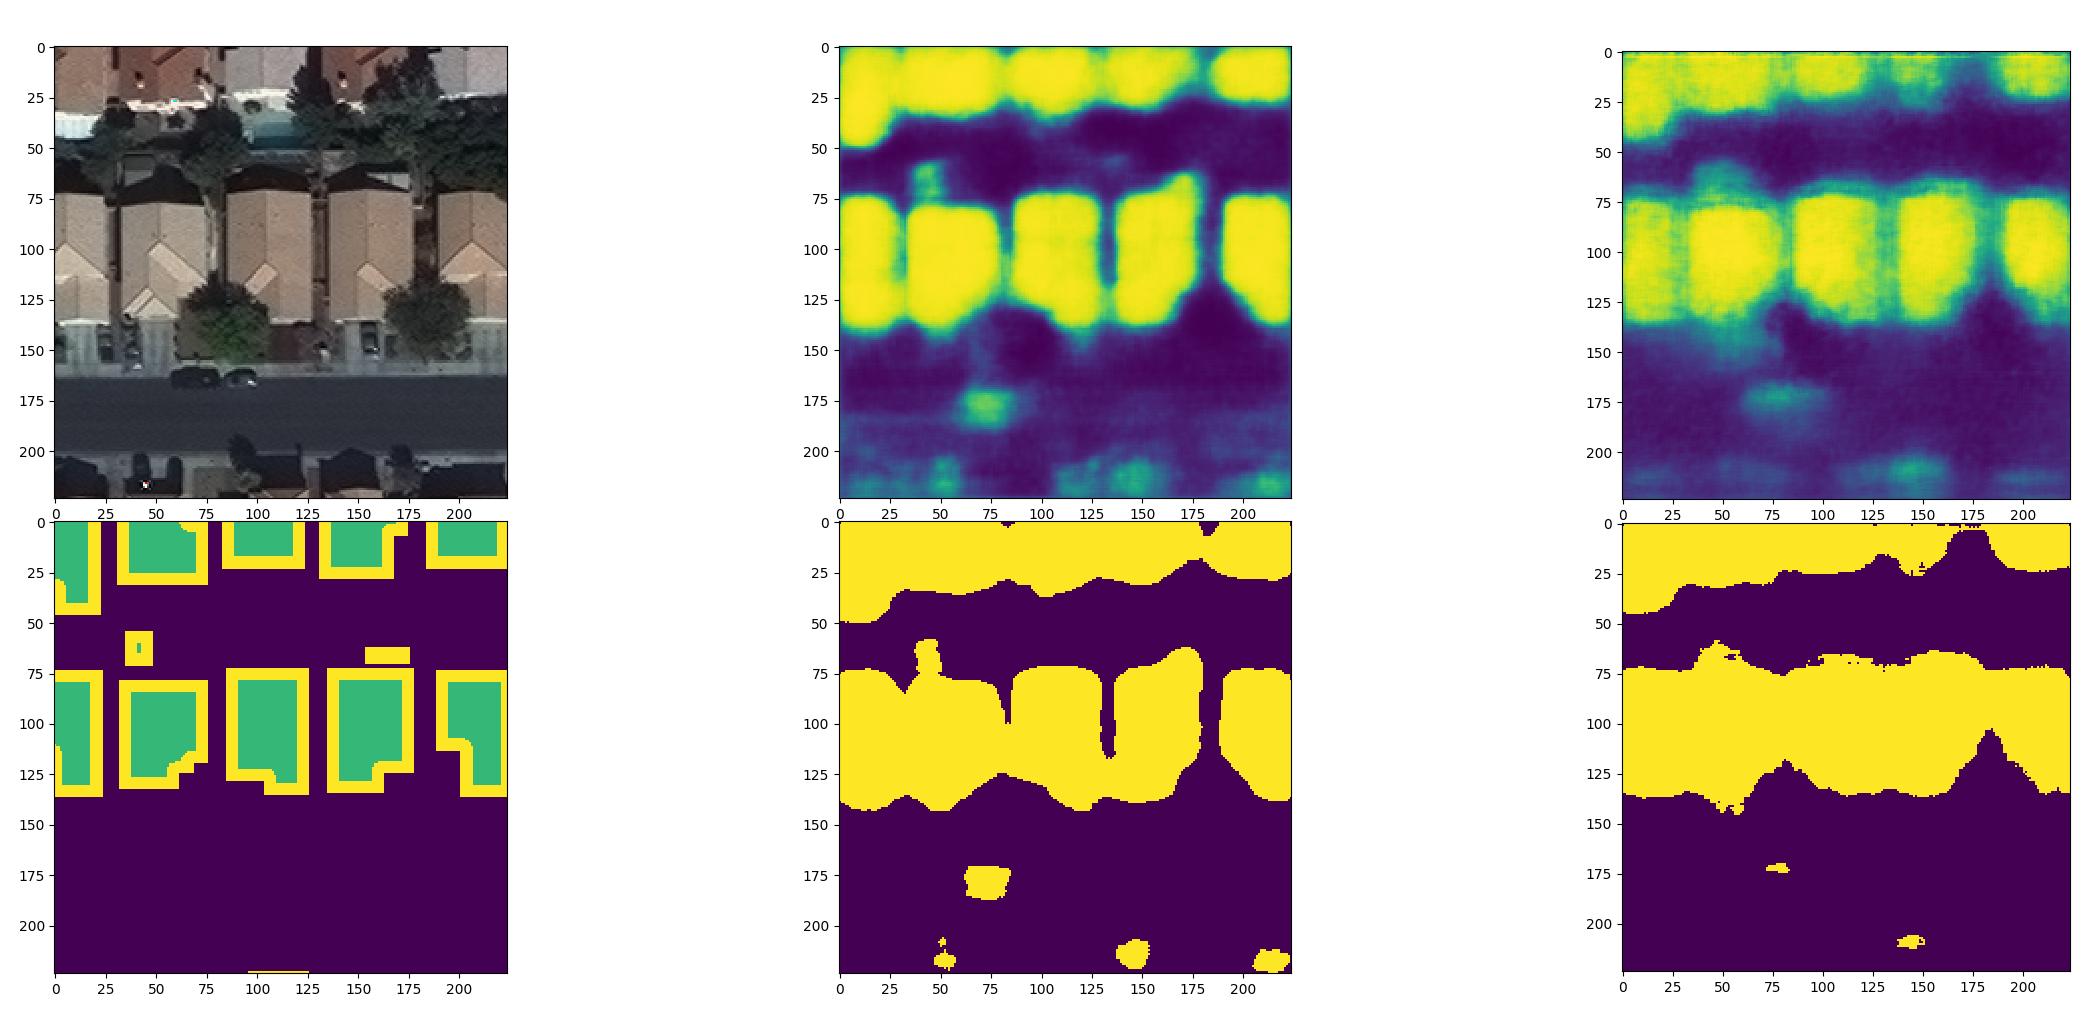
\includegraphics[scale=0.225]{Images/Deconvs_Vegas.png}
		\caption{Inférences de Deconv5 et Deconv7 sur Vegas}
	\end{center}
\end{figure}

\begin{figure}[H]
	\begin{center}
		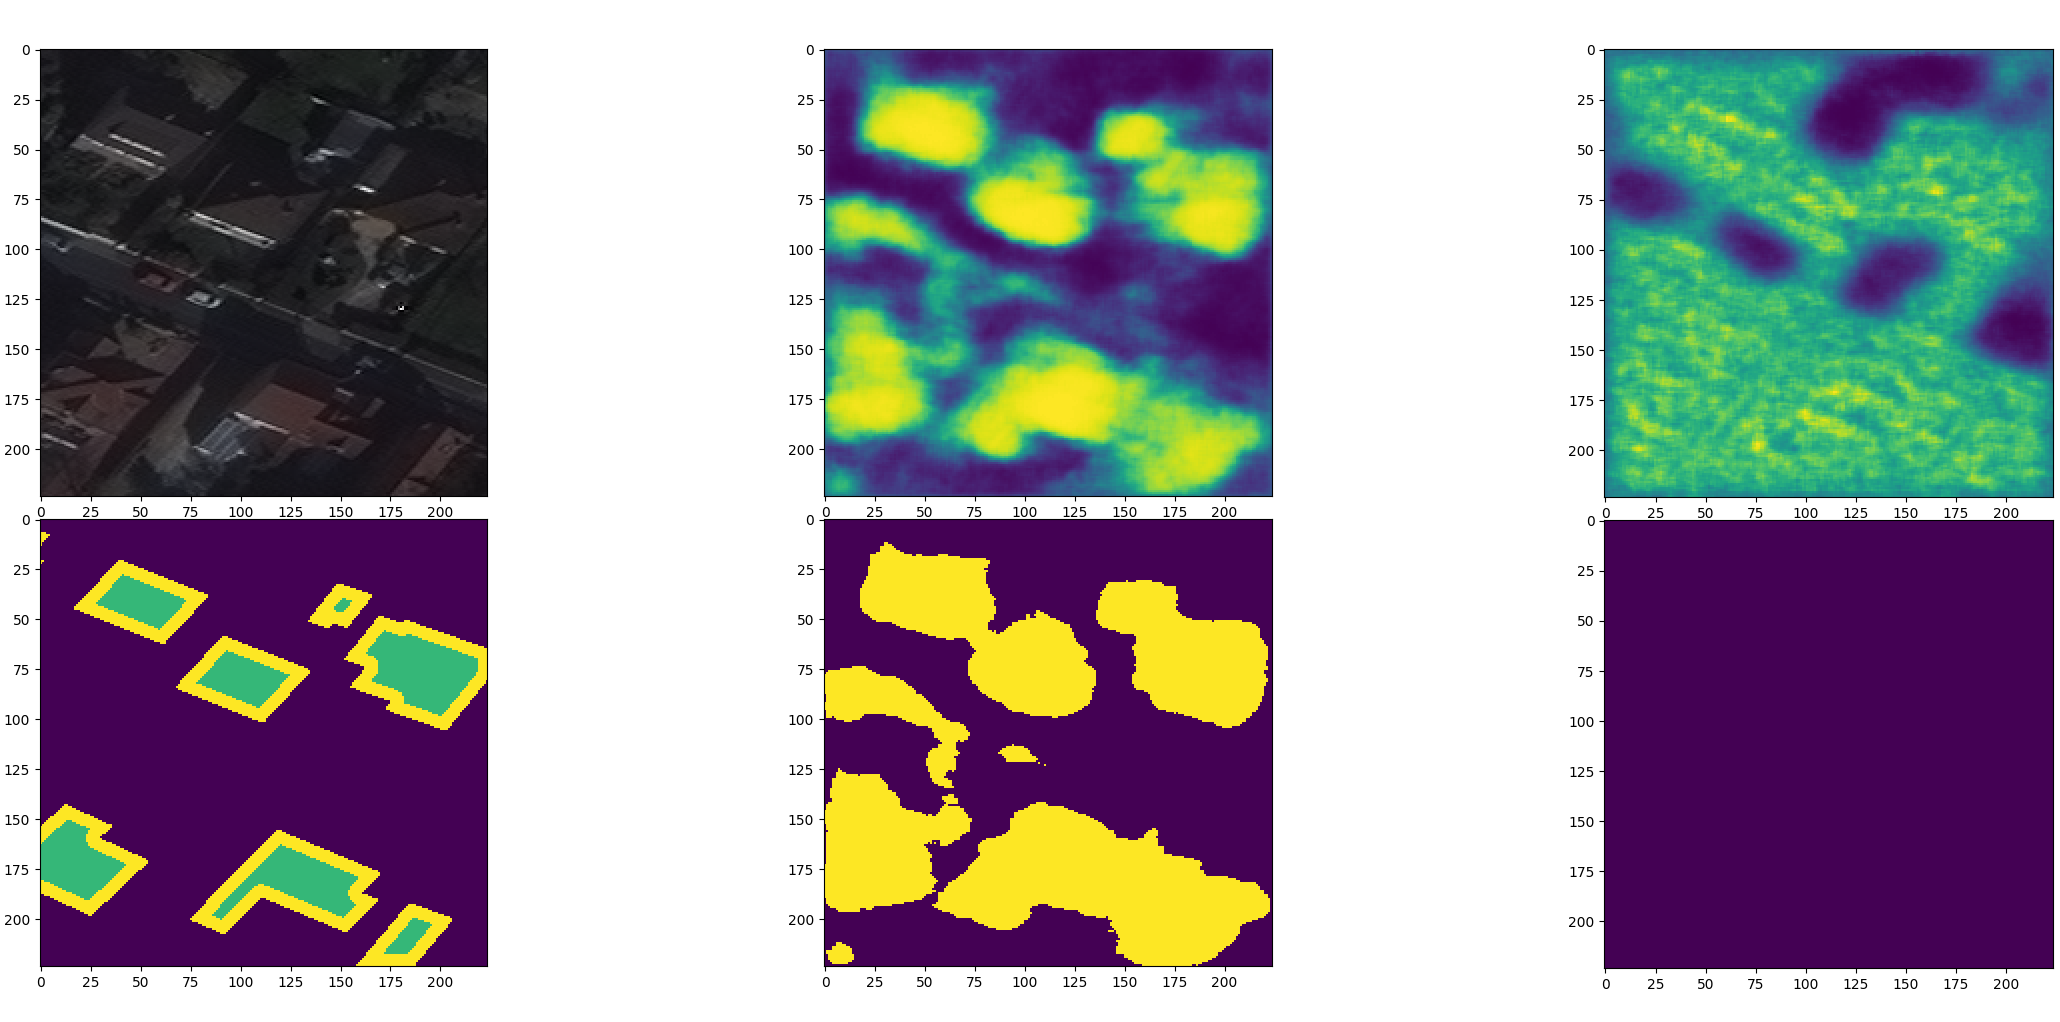
\includegraphics[scale=0.225]{Images/Deconvs_Paris.png}
		\caption{Inférences de Deconv5 et Deconv7 sur Paris}
	\end{center}
\end{figure}

\begin{figure}[H]
	\begin{center}
		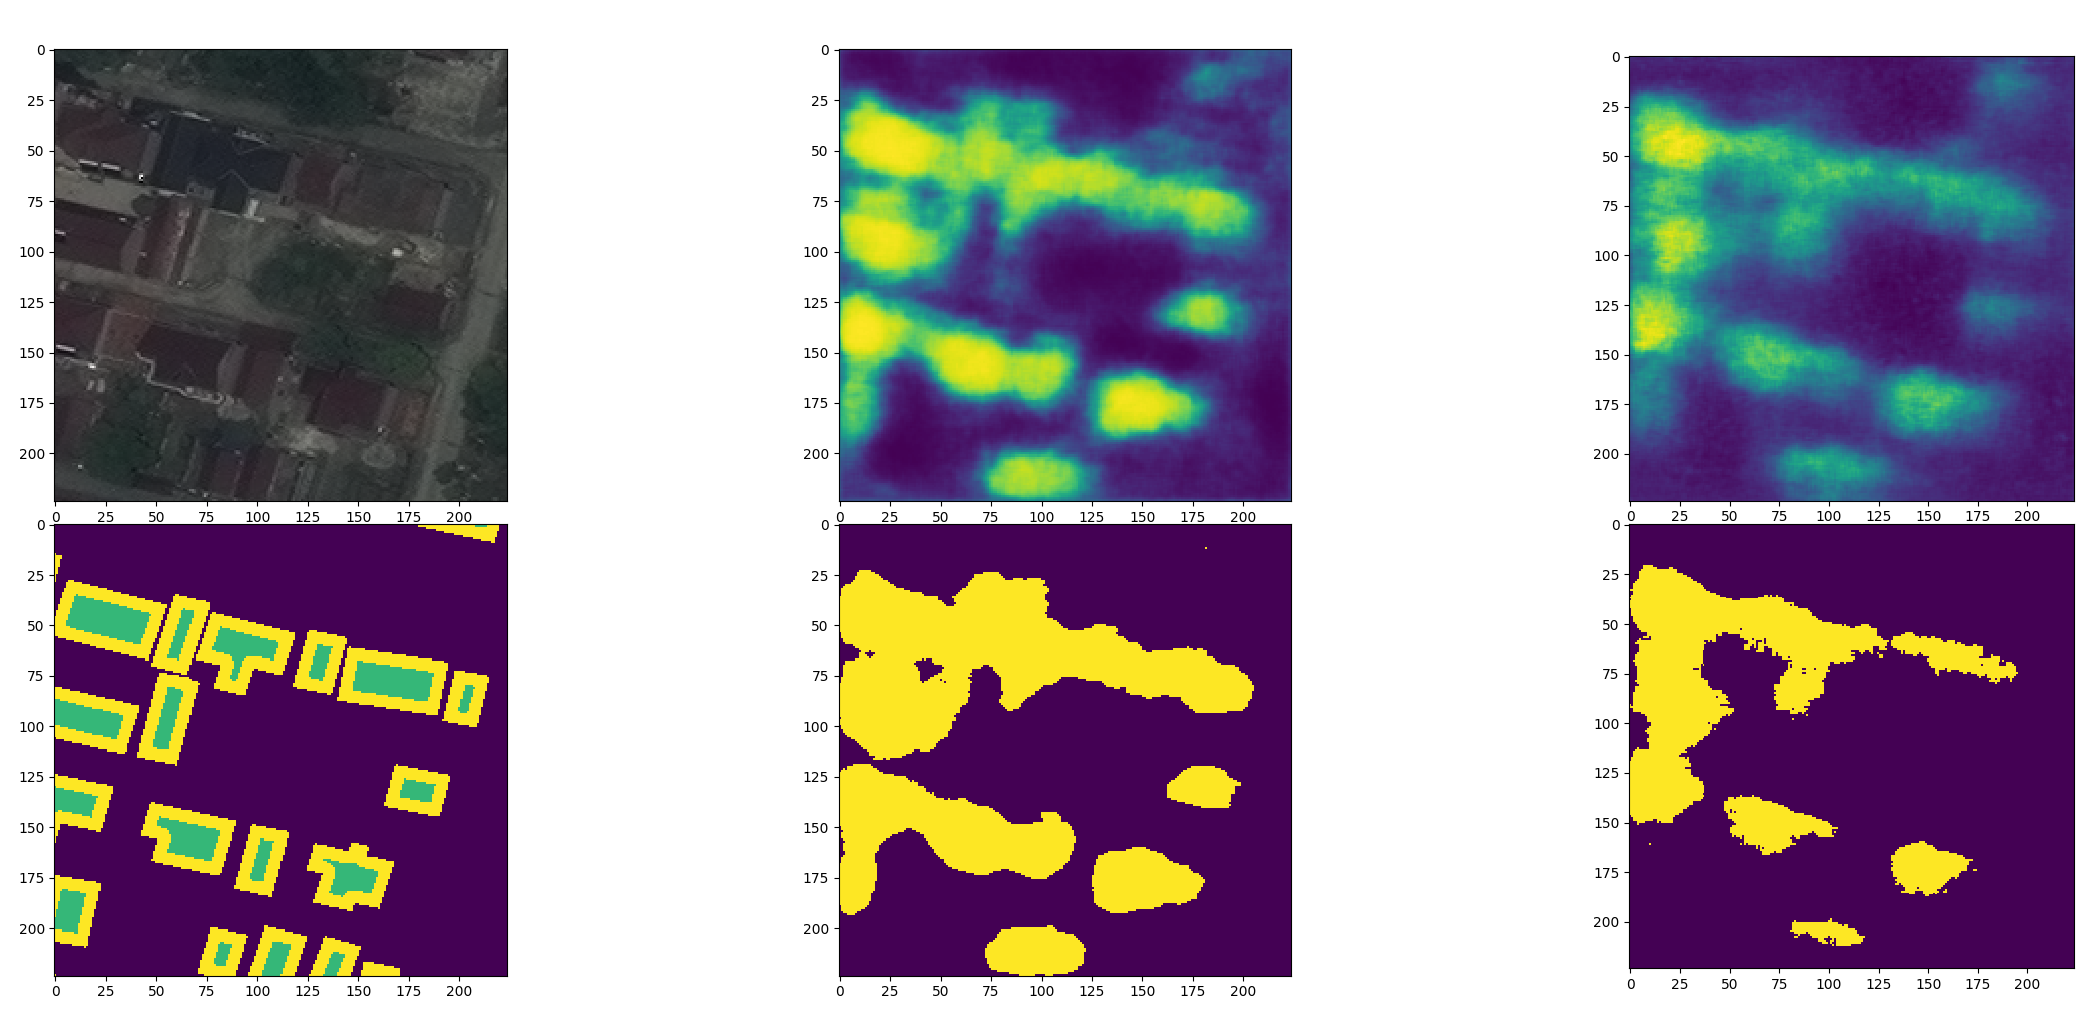
\includegraphics[scale=0.225]{Images/Deconvs_Shanghai.png}
		\caption{Inférences de Deconv5 et Deconv7 sur Shanghai}
	\end{center}
\end{figure}

\begin{figure}[H]
	\begin{center}
		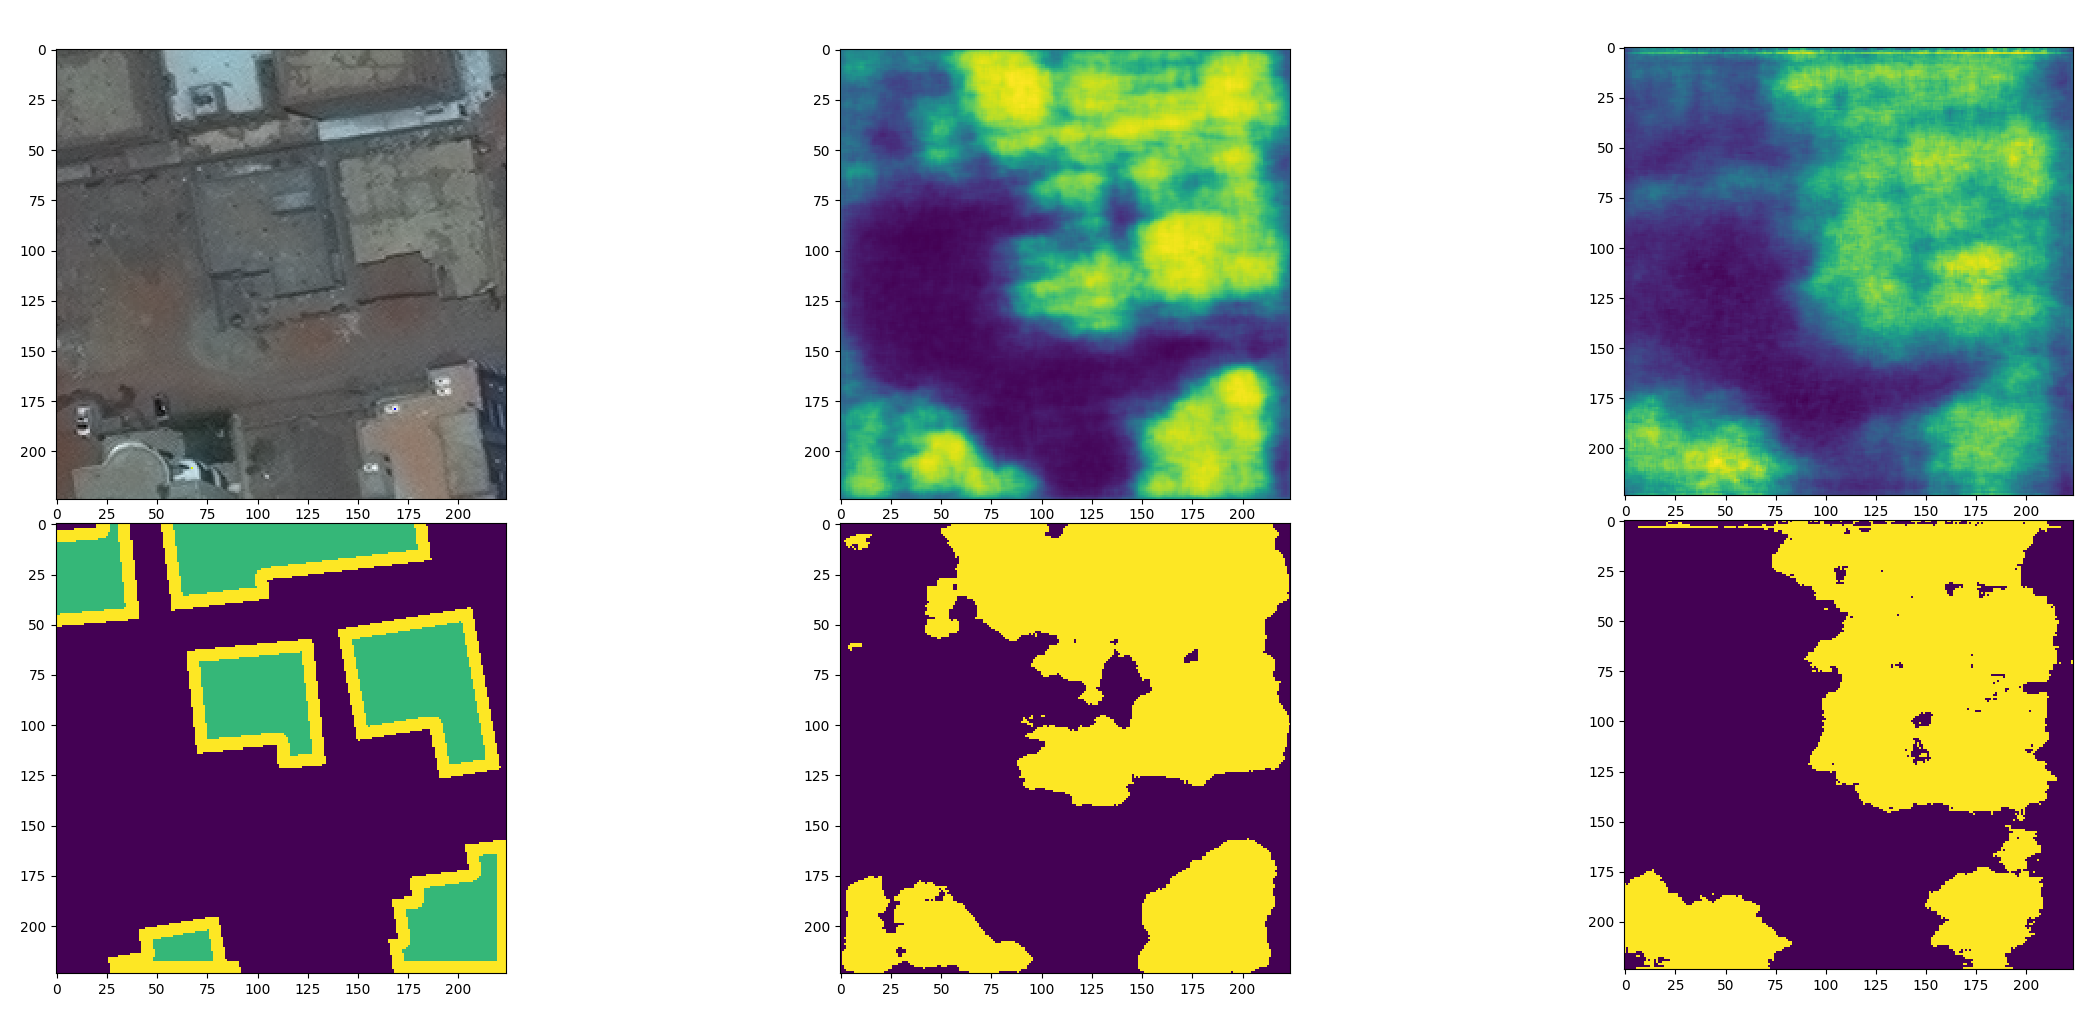
\includegraphics[scale=0.225]{Images/Deconvs_Khartoum.png}
		\caption{Inférences de Deconv5 et Deconv7 sur Khartoum}
	\end{center}
\end{figure}

On s'aperçoit sur chacun des exemples, que Deconv5 réussit systématiquement mieux que Deconv7, ce qui va dans le sens des suppositions émises dans l'analyse des résultats.
Sur Paris, la différence est flagrante, Deconv5 réalise une segmentation à peu près fidèle, tandis que la seconde est totalement fausse.

\subsubsection{Deuxième Expérience}
Une analyse empirique de la première expérience laisse suggérer que les réseaux Deconv5 et Deconv7 n'arrivent pas à considérer l'image d'entrée dans son ensemble.
En effet, commme on peut le voir, un grand bâtiment sur l'image n'est pas détecté comme un bloc unique de pixels, mais plutôt comme la réunion de plusieurs petits blocs.

Après réflexion, nous sommes arrivés à la conclusion que cela était dû au fait que le réseau ne zoomait pas assez.

Dans le cas de Deconv5, on ne s'intéresse ici qu'à la résolution de l'image et des \emph{map de features}.
Les couches \emph{pool1} et \emph{pool2}, divisent chacune la résolution de l'image par 2, soit par $2 \times 2 = 4$ après \emph{pool2}.
De ce fait, les \emph{map de features} après \emph{pool2}, ont pour résolution spatiale $(56, 56)$, un pixel de ces couches représente seulement une zone de $(4, 4)$ pixels de l'image originale.

Passons à présent aux couches \emph{conv3\_$1$} et \emph{conv3\_$2$}, ce sont toutes les deux des convolutions $(3, 3)$, ce qui équivaut grossièrement à une convolution $(5, 5)$.

On rappelle qu'une convolution s'apparente à une moyenne pondérée sur un voisinage. On comprend donc que le réseau prend en compte les \emph{features} d'un pixel et de son voisinage $(5, 5)$, et porte un "avis" quand à la nature des objets contenus dans ce voisinage.

Ici une fenêtre $(5, 5)$ de pixels, représente une zone de $(20, 20)$ pixels de l'image originale. Et c'est à peu près sur cette quantité d'information que le réseau va pouvoir juger si oui ou non la fenêtre $(5, 5)$ représente un bâtiment.

Or les données SpaceNet ont une résolution de 0.31cm, une fenêtre de pixels de dimensions $(20, 20)$ au sol représente, une zone de $6.2 \times 6.2\ m^2$, ce qui est évidemment beaucoup plus petit que la plupart des bâtiments ou maisons.

Dans cette deuxième expérience, nous avons recréé deux versions miniatures de DeconvNet.
\paragraph{Architectures}
Au lieu d'enlever des couches proche du \emph{centre de symétrie} du réseau, comme réalisé dans la première expérience, nous avons plutôt décider de compacter l'architecture DeconvNet.

Ainsi les modèles conçus réduisent plus rapidement la dimension de l'image en employant des couches de \emph{pooling} ayant un plus grand champ-récepteur.
Nous avons aussi décider de diviser par 2 le nombre de \emph{features} calculées à chaque convolution, dans le but d’accélérer les calculs.

Nous avons donc décider de créer deux modèles se différenciant sur le bloc central, en voici leur définitions :

\begin{center}
\begin{tabular}{|c|c|c|c|c|c|c|c|c|c|c|}
\hline 
Couche & \multicolumn{2}{c|}{Noyau} & \multicolumn{2}{c|}{Features} & \multicolumn{2}{c|}{Pad} & \multicolumn{2}{c|}{Stride} & \multicolumn{2}{c|}{Dimensions en sortie}\\ 
\hline 
Input & \multicolumn{2}{c|}{-} & \multicolumn{2}{c|}{-} & \multicolumn{2}{c|}{-} & \multicolumn{2}{c|}{-} & \multicolumn{2}{c|}{$(4, 224, 224)$}\\ 
\hline 
conv1\_$1$ & \multicolumn{2}{c|}{$(3, 3)$} & \multicolumn{2}{c|}{32} & \multicolumn{2}{c|}{1} & \multicolumn{2}{c|}{1} & \multicolumn{2}{c|}{$(32, 224, 224)$}\\ 
\hline
conv1\_$2$ & \multicolumn{2}{c|}{$(3, 3)$} & \multicolumn{2}{c|}{32} & \multicolumn{2}{c|}{1} & \multicolumn{2}{c|}{1} & \multicolumn{2}{c|}{$(32, 224, 224)$}\\ 
\hline 
pool1 & \multicolumn{2}{c|}{$(4, 4)$} & \multicolumn{2}{c|}{-} & \multicolumn{2}{c|}{4} & \multicolumn{2}{c|}{0} & \multicolumn{2}{c|}{$(32, 56, 56)$}\\ 
\hline 
conv2\_$1$ & \multicolumn{2}{c|}{$(3, 3)$} & \multicolumn{2}{c|}{64} & \multicolumn{2}{c|}{1} & \multicolumn{2}{c|}{1} & \multicolumn{2}{c|}{$(64, 56, 56)$}\\ 
\hline
conv2\_$2$ & \multicolumn{2}{c|}{$(3, 3)$} & \multicolumn{2}{c|}{64} & \multicolumn{2}{c|}{1} & \multicolumn{2}{c|}{1} & \multicolumn{2}{c|}{$(64, 56, 56)$}\\ 
\hline 
pool2 & \multicolumn{2}{c|}{$(4, 4)$} & \multicolumn{2}{c|}{-} & \multicolumn{2}{c|}{4} & \multicolumn{2}{c|}{0} & \multicolumn{2}{c|}{$(64, 14, 14)$}\\ 
\hline 
conv3\_$1$ & \multicolumn{2}{c|}{$(3, 3)$} & \multicolumn{2}{c|}{128} & \multicolumn{2}{c|}{1} & \multicolumn{2}{c|}{1} & \multicolumn{2}{c|}{$(128, 14, 14)$}\\ 
\hline
conv3\_$2$ & \multicolumn{2}{c|}{$(3, 3)$} & \multicolumn{2}{c|}{128} & \multicolumn{2}{c|}{1} & \multicolumn{2}{c|}{1} & \multicolumn{2}{c|}{$(128, 14, 14)$}\\ 
\hline
conv3\_$3$ & \multicolumn{2}{c|}{$(3, 3)$} & \multicolumn{2}{c|}{128} & \multicolumn{2}{c|}{1} & \multicolumn{2}{c|}{1} & \multicolumn{2}{c|}{$(128, 14, 14)$}\\ 
\hline 
pool3 & \multicolumn{2}{c|}{$(2, 2)$} & \multicolumn{2}{c|}{-} & \multicolumn{2}{c|}{2} & \multicolumn{2}{c|}{0} & \multicolumn{2}{c|}{$(128, 7, 7)$}\\ 
\hline 
conv4\_$1$ & $(3,3)$ & $(7, 7)$ & \multicolumn{2}{c|}{256} & 1 & 0 & 1 & 1 & $(256, 7, 7)$ & $(256, 1, 1)$ \\
\hline
conv4\_$2$ & $(3,3)$ & $(1, 1)$ & \multicolumn{2}{c|}{256} & 1 & 0 & 1 & 1 & $(256, 7, 7)$ & $(256, 1, 1)$ \\
\hline
deconv4\_$3$ & $(3,3)$ & $(7, 7)$ & \multicolumn{2}{c|}{128} & 1 & 0 & 1 & 1 & $(128, 7, 7)$ & $(128, 7, 7)$ \\
\hline
unpool3 & \multicolumn{2}{c|}{$(2, 2)$} & \multicolumn{2}{c|}{-} & \multicolumn{2}{c|}{2} & \multicolumn{2}{c|}{0} & \multicolumn{2}{c|}{$(128, 14, 14)$}\\ 
\hline
deconv3\_$1$ & \multicolumn{2}{c|}{$(3, 3)$} & \multicolumn{2}{c|}{128} & \multicolumn{2}{c|}{1} & \multicolumn{2}{c|}{1} & \multicolumn{2}{c|}{$(128, 14, 14)$}\\ 
\hline
deconv3\_$2$ & \multicolumn{2}{c|}{$(3, 3)$} & \multicolumn{2}{c|}{128} & \multicolumn{2}{c|}{1} & \multicolumn{2}{c|}{1} & \multicolumn{2}{c|}{$(128, 14, 14)$}\\ 
\hline
deconv3\_$3$ & \multicolumn{2}{c|}{$(3, 3)$} & \multicolumn{2}{c|}{64} & \multicolumn{2}{c|}{1} & \multicolumn{2}{c|}{1} & \multicolumn{2}{c|}{$(64, 14, 14)$}\\ 
\hline
unpool2 & \multicolumn{2}{c|}{$(4, 4)$} & \multicolumn{2}{c|}{-} & \multicolumn{2}{c|}{4} & \multicolumn{2}{c|}{0} & \multicolumn{2}{c|}{$(64, 56, 56)$}\\ 
\hline
deconv2\_$1$ & \multicolumn{2}{c|}{$(3, 3)$} & \multicolumn{2}{c|}{64} & \multicolumn{2}{c|}{1} & \multicolumn{2}{c|}{1} & \multicolumn{2}{c|}{$(64, 56, 56)$}\\ 
\hline
deconv2\_$2$ & \multicolumn{2}{c|}{$(3, 3)$} & \multicolumn{2}{c|}{32} & \multicolumn{2}{c|}{1} & \multicolumn{2}{c|}{1} & \multicolumn{2}{c|}{$(32, 56, 56)$}\\ 
\hline
unpool1 & \multicolumn{2}{c|}{$(4, 4)$} & \multicolumn{2}{c|}{-} & \multicolumn{2}{c|}{4} & \multicolumn{2}{c|}{0} & \multicolumn{2}{c|}{$(32, 224, 224)$}\\ 
\hline
deconv1\_$1$ & \multicolumn{2}{c|}{$(3, 3)$} & \multicolumn{2}{c|}{32} & \multicolumn{2}{c|}{1} & \multicolumn{2}{c|}{1} & \multicolumn{2}{c|}{$(32, 224, 224)$}\\ 
\hline
deconv1\_$2$ & \multicolumn{2}{c|}{$(3, 3)$} & \multicolumn{2}{c|}{32} & \multicolumn{2}{c|}{1} & \multicolumn{2}{c|}{1} & \multicolumn{2}{c|}{$(32, 224, 224)$}\\ 
\hline
Output & \multicolumn{2}{c|}{$(1, 1)$} & \multicolumn{2}{c|}{3} & \multicolumn{2}{c|}{1} & \multicolumn{2}{c|}{0} & \multicolumn{2}{c|}{$(3, 224, 224)$}\\ 
\hline
\end{tabular} 
\end{center}
Les différences par rapport à la première expérience sont l'utilisation de couche de \emph{pooling} ayant un noyau $(4, 4)$ et un pas de déplacement de 4, permettant de réduire rapidement les dimensions des \emph{map de features}.

Les différences entre les deux modèles se font au niveau du bloc central, dans l'un, l'information reste spatialisée, nous opérons seulement deux convolutions $(3, 3)$ comme dans l'expérience précédente et dans l'autre, nous reprenons un bloc similaire à celui de DeconvNet.
\paragraph{Hyper-paramètres}
Les hyper-paramètres restent les même par rapport à l'expérience précédente.
\paragraph{Résultats}
\subparagraph{Graphes des Pertes}
Voici le graphe des pertes du modèle ZoomNet :
\begin{figure}[H]
	\begin{center}
		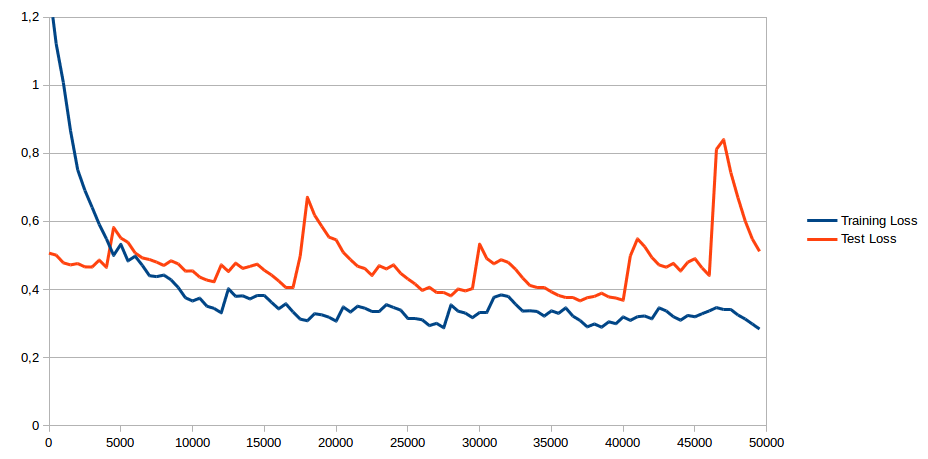
\includegraphics[scale=0.6]{Images/Losses_ZoomNet.png}
		\caption{Graphe de la fonction de perte pour le modèle ZoomNet}
	\end{center}
\end{figure}
L'écart entre l'erreur d'apprentissage et l'erreur de test reste faible avant l'itération 40000, on peut donc conclure qu'il n'y a peu ou pas de sur-apprentissage avant 40000 itérations.
De plus l'erreur varie de façon peu erratique, ce qui est signe d'un bon apprentissage.

Voici le graphe des pertes du modèle ZoomNet2 :
\begin{figure}[H]
	\begin{center}
		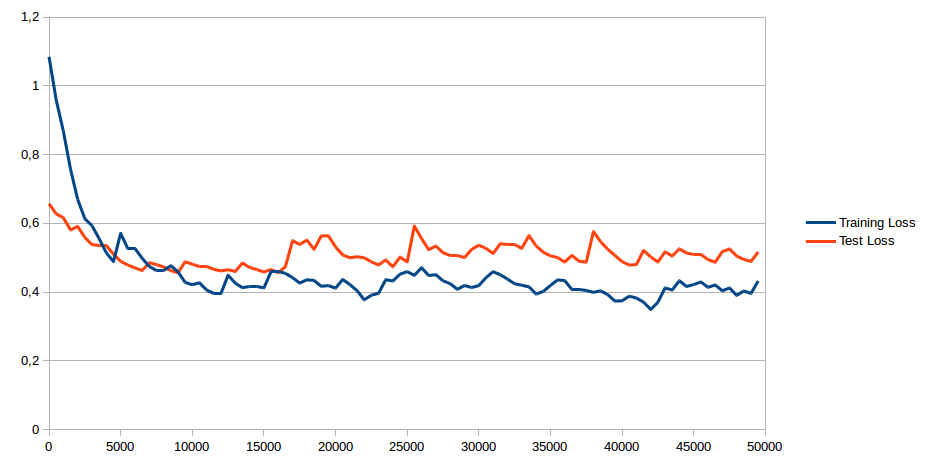
\includegraphics[scale=0.6]{Images/Losses_ZoomNet2.png}
		\caption{Graphe de la fonction de perte pour le modèle ZoomNet2}
	\end{center}
\end{figure}
L'écart entre l'erreur d'apprentissage et l'erreur de test est faible, on peut donc conclure qu'il n'y a peu ou pas de sur-apprentissage.
De plus l'erreur ne varie pas de façon particulièrement erratique, ce qui est signe d'un bon apprentissage.
\subparagraph{Analyse des Résultats}
Voyons à présent les meilleures performances des modèles.

La précision est calculée de la même façon que précédemment.

Pour ZoomNet, l'itération 37000 semble être la meilleure.

La précision globale est de $0.83479$.

La matrice de confusion est la suivante :
\begin{center}
	\begin{tabularx}{0.5\textwidth}{c|c c c|}
		Réel/Prédit & Bâtiment & Route & Absence \\
		\hhline{----}
		Bâtiment & 0.825 \cellcolor[gray]{.8} & \multicolumn{2}{c|}{0.175} \\
		Route & 0.262* & 0.738 \cellcolor[gray]{.8} & 0.262*\\
		Absence & \multicolumn{2}{c}{0.176} & 0.824 \cellcolor[gray]{.8}\\
		\hhline{~---}
	\end{tabularx}
\end{center}

La matrice de confusion n'est pas complète, car Caffe ne produit pas l'ensemble des informations lors de l'évaluation du modèle.

L'étoile, *, signifie que la valeur est partagée entre les deux champs.

Pour ZoomNet2, l'itération 34000 semble être la meilleure.

La précision globale est de $0.777292$.

La matrice de confusion est la suivante :
\begin{center}
	\begin{tabularx}{0.5\textwidth}{c|c c c|}
		Réel/Prédit & Bâtiment & Route & Absence \\
		\hhline{----}
		Bâtiment & 0.868 \cellcolor[gray]{.8} & \multicolumn{2}{c|}{0.132} \\
		Route & 0.278* & 0.722 \cellcolor[gray]{.8} & 0.278*\\
		Absence & \multicolumn{2}{c}{0.25} & 0.75 \cellcolor[gray]{.8}\\
		\hhline{~---}
	\end{tabularx}
\end{center}

De ces deux modèles, le premier semble plus performant que le second, ce qui indique peut être que garder l'information spatialisée sur le bloc central est important.
\subparagraph{Exemples de Résultats}
Nous allons à présent comparer les résultats produits par ZoomNet et ZoomNet2.

\begin{figure}[H]
	\begin{center}
		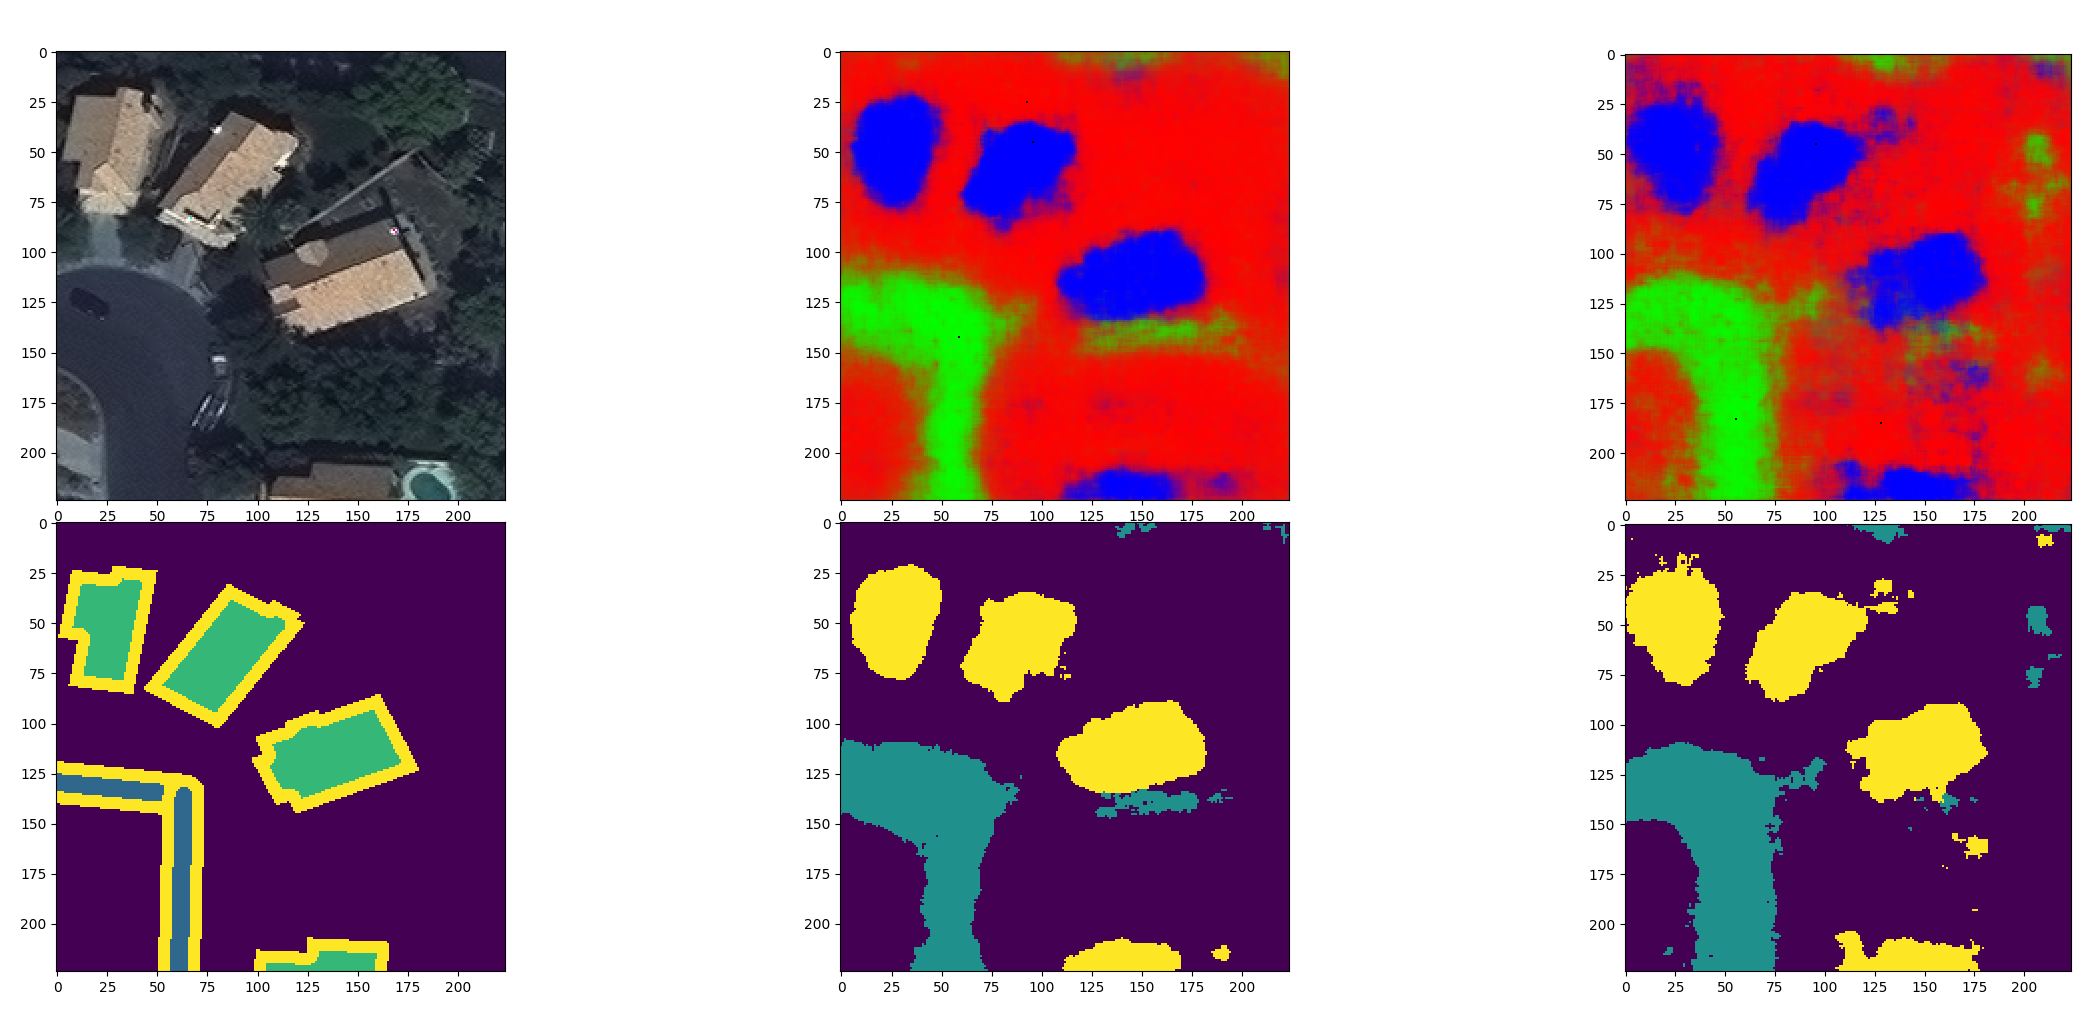
\includegraphics[scale=0.225]{Images/ZoomNets_1983.png}
		\caption{Inférences de ZoomNet et ZoomNet2}
	\end{center}
\end{figure}

En haut à gauche, l'image de SpaceNet, bandes RGB, corrigée 8bits.

En bas à gauche, le masque de segmentation produit par les labels de SpaceNet et OpenStreetMap.

En haut au milieu, la \emph{map} de probabilités de ZoomNet, représentée comme une image RGB.

En bas au milieu, le masque de segmentation de ZoomNet, obtenu en récupérant l'\emph{argmax} de la \emph{map} de probabilité.

En haut à droite, la \emph{map} de probabilités de ZoomNet2, représentée comme une image RGB.

En bas à droite, le masque de segmentation de ZoomNet2, obtenu en récupérant l'\emph{argmax} de la \emph{map} de probabilité.

On voit pour cette image, que le résultat est beaucoup plus "propre" pour le premier modèle que le second, il y a moins bruit de segmentation sur la sortie, c'est à dire de petites tâches n'ayant pas lieu d'être.

\begin{figure}[H]
	\begin{center}
		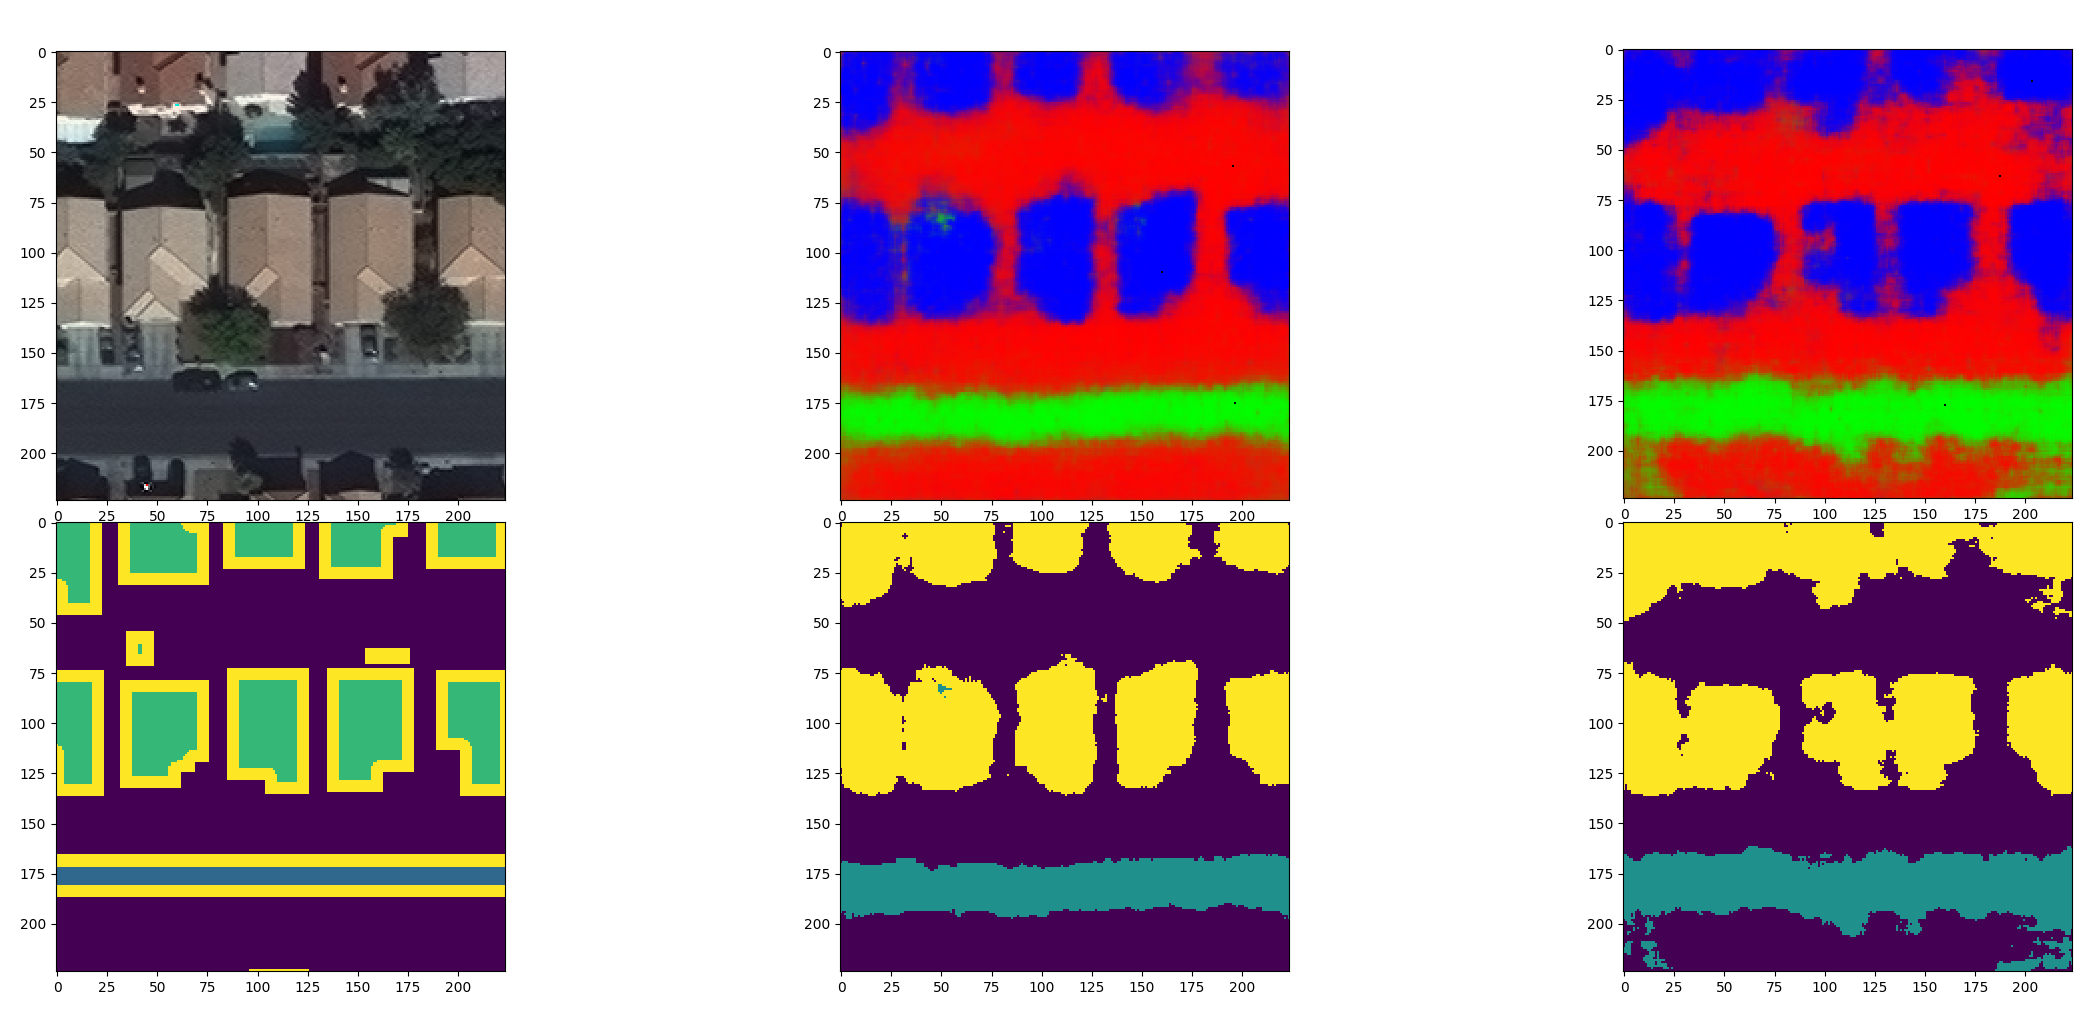
\includegraphics[scale=0.225]{Images/ZoomNets_5000.png}
		\caption{Inférences de ZoomNet et ZoomNet2}
	\end{center}
\end{figure}

Pour cet exemple, le résultat semble toujours meilleur dans le cas où l'information reste spatialisée, en effet, le contour des bâtiments est beaucoup plus précis, même dans les cas où les bâtiments sont collés. Il y aussi moins d'artefacts sur la route.
\subsection{Conclusion}
Dans cette partie, nous avons décrit l'utilisation de l'apprentissage profond pour de la cartographie automatisée.

Nous avons vu différentes raisons motivant l'usage de la cartographie automatisée, présenté les données issues de SpaceNet croisées avec la base de données OpenStreetMap, et expliqué brièvement l'opération de rasterisation, permettant la transformation de données vectorielles en données matricielles.

Nous avons succinctement évoqué les motivations concernant le calcul sur GPU, et présenté le \emph{framework} d'apprentissage profond Caffe, utilisé pour nos modèles.

Puis, nous avons présenté l'architecture DéconvNet,ayant inspiré nos modèles de segmentation.

Notre première expérience qui consistait à prédire des masques de segmentation des bâtiments sur l'ensemble des données de SpaceNet était satisfaisante, même si les modèles créés, Deconv5 et Deconv7, souffraient de vision tunnelisée.

La seconde expérience consistait à prédire des masques de segmentation des bâtiments et des routes sur la zone géographique de Las Vegas.
Cette expérience a tenté de corriger ce défaut en agrandissant la fenêtre et la stride des couches de \emph{pooling}, permettant considérer l'image dans son ensemble.
Deux modèles ont été créés, ZoomNet et ZoomNet, se différenciant sur le bloc central, le premier gardant l'information spatialisée, le second la dé-spatialisant.
Les résultats obtenus sont de meilleure qualité que ceux obtenus dans la première expérience, car plus fins et moins bruités.

Ces deux expériences nous permettent alors de formuler des règles empiriques quand à l'importance de réduire la dimensionnalité des données pour éviter le problème de vision tunnelisée, ainsi que formuler l'hypothèse de garder l'information spatialisée dans le bloc central.
\section{Recherche de Similarités}

Une piste envisagée au début du stage était de proposer une solution réalisant de la classification d'images en proposant une méthode partiellement supervisée, appelée classification dynamique de \emph{patchs} d'images.
Un patch d'une image satellite est une sous-région de l'image satellite.

Nous verrons ensuite des résultats de recherche de similarités dans le cas d'images satellite.

\subsection{Classification Dynamique}
La classification dynamique se décompose en trois étapes :
\begin{enumerate}
	\item L'entraînement d'un modèle à une tâche de vision par ordinateur quelconque.
	\item La création semi-supervisée d'un \emph{dataset} de classification d'images.
	\item L'entraînement d'un second modèle à la classification d'images sur le \emph{dataset} précédemment créé.
\end{enumerate}

\subsubsection{Première Étape : Classification Générique d'Images}
Nous avons décidé d'entraîner des modèles à la classification d'images, car c'est la tâche de vision la plus élémentaire, et sans doute la plus facile.

Pour la première partie, nous avons mené deux expériences :
\begin{itemize}
	\item Entraîner un modèle de classification sur le \emph{dataset} CIFAR-10.
	\item Réutiliser un modèle déjà entraîné sur le \emph{dataset} ImageNet.
\end{itemize}

\paragraph{Première Expérience}
La première expérience avait pour but principal de se familiariser avec TensorFlow, un framework développé par Google.

Le modèle créé était une version "miniaturisée" de VGG-16, adaptée pour classifier des images de dimension $(3, 32, 32)$ issues de CIFAR-10 en 10 catégories.

\paragraph{Seconde Expérience}
La seconde expérience réutilisait le modèle VGG-16, déjà entraîné sur ImageNet.

\subsubsection{Deuxième Étape : Création Semi-Supervisée d'un Dataset}
L'étape de création semi-supervisée d'un \emph{dataset} s'apparentait réellement à de la recherche de similarités entre images.

L'idée est simple, le calcul du coefficient de corrélation de Pearson  est une mesure de la corrélation entre deux variables.

Il se calcule de la façon suivante :
$$\rho_{X,Y} = \frac{cov(X,Y)}{\sigma_X \sigma_Y}$$
Avec $cov(X,Y)$, la covariance entre $X$ et $Y$ et $\sigma_X$, $\sigma_Y$, les variances respectives de $X$ et $Y$.

Une approche naïve pourrait suggérer de directement calculer la matrice des corrélations entre les images à traiter. Malheureusement, les images satellite sont naturellement bruitées, à cause entre autre de la végétation, des reliefs, etc.
On sait cependant que les réseaux de neurones entraînés une tâche de vision par ordinateur sont capables d'extraire des informations importantes d'une image, en faisant abstraction du bruit.
On parle alors d'extraction de \emph{features} d'une image.
En effet, nous avons vu dans le chapitre portant sur l'apprentissage profond, qu'une image est décomposée en \emph{maps de features} successives.
Ainsi, au lieu de calculer la matrice de corrélations directement entre les images, nous pouvons plutôt calculer la matrice des corrélations entre les décompositions en \emph{features} des images.

Ce nouveau calcul de corrélations revient à effectuer une \emph{recherche de similarités entre images} si la décomposition en \emph{features} est "sensée".


Il nous faut ensuite récupérer les images les plus corrélées entre elles et les placer dans différentes classes, en utilisant par exemple le $k$\emph{-means clustering}, permettant ainsi la création d'un \emph{dataset}.

\subsubsection{Troisième Étape : Classification d'Images}

La troisième étape est très simple, il suffit juste d'effectuer l'apprentissage d'un modèle de classification le \emph{dataset} précédemment créé.

Nous n'avons pas réalisé cette étape, car nous n'avions pas suffisamment de données à l'époque.

\subsection{Analyse des Résultats}
L'image utilisée pour la recherche de similarités est une image de Commerce City, Colorado, États-Unis, provient du satellite Pléiades.

Les dimensions de l'image sont $(4, 14029, 14012)$, la résolution est de 0.5m, l'image occupe 1.6Go sur le disque.

Nous n’utiliserons que 3 des 4 bandes disponibles, les bandes Rouge, Vert et Bleu, car le modèle VGG-16 n'a été entraîné que sur des images RGB.

\begin{figure}[H]
	\begin{center}
		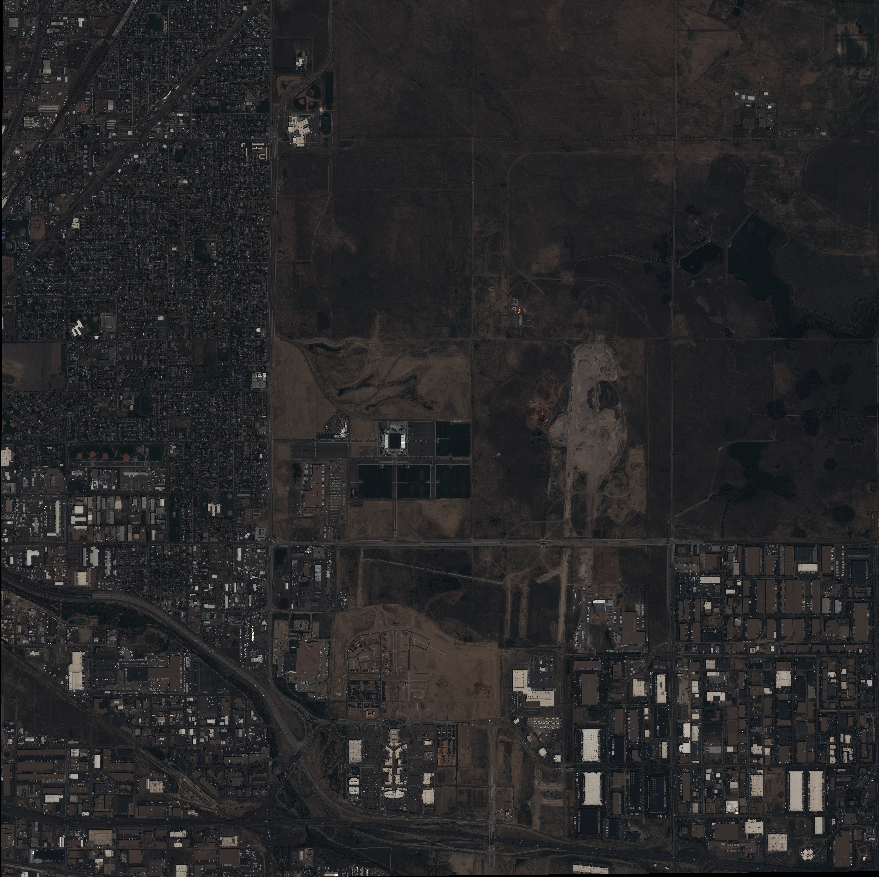
\includegraphics[scale=0.9]{Images/CommerceCity.png}
		\caption{Image (RGB, 8bits, Correction $[2-98]\%$) de Commerce City}
	\end{center}
\end{figure}

L'image a été découpée en 47742 \emph{patchs} de dimensions $(3, 64, 64)$, interpolés aux dimensions $(3, 32, 32)$, puis décomposés en \emph{features} à différents niveaux par le premier modèle, entraîné sur CIFAR-10.

Nous avons ensuite calculé la matrice des corrélations des 47742 décomposition en \emph{features} des images.

L'image en haut à gauche est l'image de référence, puis de gauche à de droite et de haut en bas, sont les 8 images les plus corrélées.

\begin{figure}[H]
	\begin{center}
		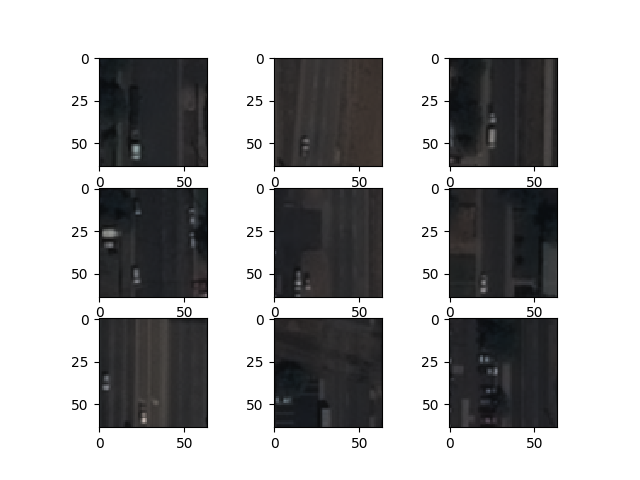
\includegraphics[scale=0.9]{Images/CommerceCity_Correlation_1.png}
		\caption{Exemples de corrélation de \emph{patchs} décomposés en \emph{features} de bas niveau}
	\end{center}
\end{figure}

\begin{figure}[H]
	\begin{center}
		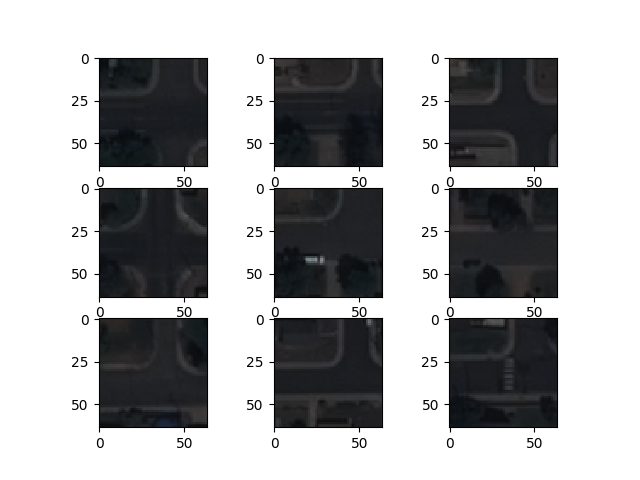
\includegraphics[scale=0.9]{Images/CommerceCity_Correlation_2.png}
		\caption{Exemples de corrélation de \emph{patchs} décomposés en \emph{features} de haut niveau}
	\end{center}
\end{figure}

Comme on peut le remarquer sur les deux figures, les images sont globalement similaires.

Toutefois, pour la première figure, on remarque que les similarités entre les patchs sont au niveau de la localisation des voitures, qui sont de petits éléments dans l'image.

À l'inverse dans la seconde figure, les patchs similaires ont en commun un croisement entre deux routes, mais que la position des arbres ou la présence de voitures ne présentent pas d'importance.
\subsection{Conclusion}
Dans cette partie nous avons décrit le concept de recherche de similarités dans les images.

Nous avons dans un premier temps souhaité réaliser de la classification dynamique d'images.
Cette application ne sera finalement pas complètement réalisée, d'une part par un manque de données, et d'autre part car l'intérêt de cette application est faible.
En effet, classifier des patchs d'images est bien moins intéressant en terme de précision que de segmenter ces mêmes patchs.
C'est pourquoi, nous n'avons pas décider de nous attarder sur cette tâche et de nous tourner vers la segmentation d'images, développée plus haut.

Toutefois, le concept de recherche de similarités reste intéressant indépendamment de la classification dynamique pour au moins deux raisons :
\begin{itemize}
	\item L'extraction de \emph{features} peut se faire sur la sortie de n'importe quelle couche de n'importe quel modèle, permettant de décomposer l'image en \emph{features} de plus ou moins haut niveau et permettant ainsi d'observer plusieurs niveaux de similarités.
	\item 
\end{itemize}
\chapter{Conclusion}
\chapter*{Bibliographie}
\begin{itemize}
	\item Deep Learning : \url{http://deeplearning.net/}
	\item Deep Learning Book : \url{http://www.deeplearningbook.org/}
	\item Neural Networks and Deep Learning : \url{http://neuralnetworksanddeeplearning.com/}
\end{itemize}
\chapter*{Annexes}
\section{Algorithme de Descente de Gradient : Adam}
La méthode \emph{Adam}, signifiant \emph{Adaptative Moment Estimation}, est une amélioration de la méthode \emph{RMSProp}.\\
Cette méthode utilise à la fois le concept de moyenne mobile ainsi que le concept d'utilisation des moments, c'est à dire d'utiliser aussi les gradients précédents :
$$\theta_{k+1} = \theta_k - \alpha \nabla_\theta J(x,y,\theta_k) - \beta \nabla_\theta J(x,y,\theta_{k-1})$$

On définit alors la matrice $G_k$ :
$$G_k = \gamma G_{k-1} + (1-\gamma)(\nabla_\theta J(x,y,\theta_k)\odot\nabla_\theta J(x,y,\theta_k)) \times I_n$$
On définit par ailleurs $m_k$, le moment du gradient $\nabla_\theta J(x,y,\theta)$, tel que :
$$m_k = \beta m_{k-1} + (1-\beta) \nabla_\theta J(x,y,\theta_k) $$
On peut remarquer que $m_k$ est lui même une moyenne mobile des gradients.
Nous utiliserons alors les estimateurs non-biaisés de $m_k$ et $G_k$ :
$$\hat{m}_k = \frac{m_k}{1-\beta^k} $$
et
$$\hat{G}_k = \frac{G_k}{1-\gamma^k}$$
Ainsi à chaque itération, nous appliquerons à $\theta$, la formule suivante :
$$\theta_{k+1} = \theta_k - \alpha (\hat{G}_k)^{-\frac{1}{2}} \hat{m}_k$$
Nous avons alors l'algorithme suivant :
\begin{algorithm}[H]
	\caption{Algorithme de Descente de Gradient Stochastique utilisant \emph{Adam}}
	\begin{algorithmic}
	    \REQUIRE {
	    $x$ et $y \in \mathbb{R}^n$,\\
	    $m < n$,\\
	    $\theta_0$, les paramètres initiaux du modèle, initialisés aléatoirement,\\
	    $\beta = 0.9$, $\gamma = 0.999$, $\alpha = 0.001$.\\
	    et $\epsilon > 0$, seuil de tolérance.
	     }
	    \REPEAT
	    	\STATE $\hat{x},\hat{y} = sample(x,y,m)$
	    	\STATE Calcul de $\nabla_\theta J(\hat{x},\hat{y},\theta_k)$.
	    	\STATE $m_k = \beta m_{k-1} + (1-\beta) \nabla_\theta J(x,y,\theta_k)$
	    	\STATE $\hat{m}_k = \frac{m_k}{1-\beta^k} $
	    	\STATE $G_k = \gamma G_{k-1} + (1-\gamma)\nabla_\theta J(x,y,\theta_k)\odot\nabla_\theta J(x,y,\theta_k) \times I_n$
	    	\STATE $\hat{G}_k = \frac{G_k}{1-\gamma^k}$
	    	\STATE $\theta_{k+1} = \theta_k - \alpha (\hat{G}_k)^{-\frac{1}{2}} \times \hat{m}_k$
	    \UNTIL{$\nabla_\theta J(\hat{x},\hat{y},\theta_k) \leq \epsilon$}
	    \RETURN $\theta_{k+1}$
	\end{algorithmic}
\end{algorithm}
Nous retiendrons cet algorithme pour résoudre les problèmes d'optimisation pour deux raisons :
\begin{itemize}
	\item Il ne nécessite pas de pas de paramétrisation, si ce n'est le choix de la taille des mini-lots $m$, ne nécessitant peu de tests.
	\item Il offre une convergence très rapide, grâce à la méthode des moments, et stable, grâce à la normalisation non biaisée du gradient $\nabla_\theta J(x,y,\theta)$.
\end{itemize}
\end{document}